\documentclass{report}

\usepackage[utf8]{inputenc}
\usepackage{titlesec}
\usepackage{easylist}
\usepackage{hanging}
\usepackage{hyperref}
\usepackage[a4paper,top=2.5cm,bottom=1.8cm,left=2.5cm,right=2.5cm]{geometry}
\usepackage{blindtext}
\usepackage{tipa}
\usepackage{epigraph}
\usepackage{enumerate}
\usepackage{longtable}
\usepackage{setspace}
\usepackage{verbatim}
\usepackage[T1]{fontenc}
\usepackage{graphicx}
\usepackage[italian]{babel}
\usepackage{amsmath}
\usepackage{pbox}
\usepackage{fancyhdr}
\usepackage{cancel}
\usepackage{tabularx}
\usepackage{booktabs}
\usepackage{multirow}
\usepackage{longtable}
\usepackage{tikz}
\usepackage{tikz-qtree}
\usepackage{subfig}
\usepackage[rgb]{xcolor}
\usepackage{amssymb}
\usepackage{mathrsfs}
\usepackage{textcomp}
\usepackage{verbatim}

% algoritmi pseudo
\usepackage[]{algorithm2e}

\usepackage{pgfplots}

\usepackage{listings}
\usepackage{color}

\definecolor{mygreen}{rgb}{0,0.6,0}
\definecolor{mygray}{rgb}{0.5,0.5,0.5}
\definecolor{mymauve}{rgb}{0.58,0,0.82}

\lstset{ 
  backgroundcolor=\color{white},   % choose the background color; you must add \usepackage{color} or \usepackage{xcolor}; should come as last argument
  basicstyle=\footnotesize,        % the size of the fonts that are used for the code
  breakatwhitespace=false,         % sets if automatic breaks should only happen at whitespace
  breaklines=true,                 % sets automatic line breaking
  captionpos=b,                    % sets the caption-position to bottom
  commentstyle=\color{mygreen},    % comment style
  deletekeywords={...},            % if you want to delete keywords from the given language
  escapeinside={\%*}{*)},          % if you want to add LaTeX within your code
  extendedchars=true,              % lets you use non-ASCII characters; for 8-bits encodings only, does not work with UTF-8
  firstnumber=1000,                % start line enumeration with line 1000
  frame=single,	                   % adds a frame around the code
  keepspaces=true,                 % keeps spaces in text, useful for keeping indentation of code (possibly needs columns=flexible)
  keywordstyle=\color{blue},       % keyword style
  language=Octave,                 % the language of the code
  morekeywords={*,...},            % if you want to add more keywords to the set
  numbers=left,                    % where to put the line-numbers; possible values are (none, left, right)
  numbersep=5pt,                   % how far the line-numbers are from the code
  numberstyle=\tiny\color{mygray}, % the style that is used for the line-numbers
  rulecolor=\color{black},         % if not set, the frame-color may be changed on line-breaks within not-black text (e.g. comments (green here))
  showspaces=false,                % show spaces everywhere adding particular underscores; it overrides 'showstringspaces'
  showstringspaces=false,          % underline spaces within strings only
  showtabs=false,                  % show tabs within strings adding particular underscores
  stepnumber=2,                    % the step between two line-numbers. If it's 1, each line will be numbered
  stringstyle=\color{mymauve},     % string literal style
  tabsize=2,	                   % sets default tabsize to 2 spaces
  title=\lstname                   % show the filename of files included with \lstinputlisting; also try caption instead of title
}

\linespread{1.2} % l'interlinea

\frenchspacing

\newcommand{\abs}[1]{\lvert#1\rvert}

\usepackage{floatflt,epsfig}

\usepackage{multicol}
\newcommand\yellowbigsqcup[1][\displaystyle]{%
  \fboxrule0pt
  \ifx#1\textstyle\fboxsep-0.6pt\else\fboxsep-1.25pt\fi
  \mathrel{\fcolorbox{white}{yellow}{$#1\bigsqcup$}}}

\newtheorem{nota}{Nota}[section]
\newtheorem{descrizione}{Descrizione}[section]
\newtheorem{notab}{Nota bene}[section]
\newtheorem{esempio}{Esempio}[section]
\newtheorem{defi}{Definizione}[section]

\title{Laboratory of image processing for computer vision}
\author{Nicola Ferru}
\begin{document}
\maketitle
\tableofcontents
\chapter{Introduzione}
\label{chap:intro}
\begin{defi}
  GNU/Octave è un applicativo per il calcolo matriciale che consente di svilgere
  tutte le operazioni base e non solo a riguardo, dallo somma, divisione,
  moltiplicazioni e sottrazioni tra matrici, calcolo del determinante, del
  grado e tanto altro.
\end{defi}

\section{Pacchetti e impostazioni base}
\label{sec:packbase}

\subsection{Pacchetti}
\label{sec:pack}

\begin{table}[th]
  \centering
  \begin{tabular}{ll}
    {\bf Nome} & {\bf Descrizione}\\\hline
    \href{https://gnu-octave.github.io/packages/fuzzy-logic-toolkit/}{fuzzy-logic-toolkit} & Un toolkit di logica fuzzy per lo più
                                                                                               compatibile con MATLAB per Octave \\\hline
    \href{https://gnu-octave.github.io/packages/symbolic/}{symbolic} & Aggiunge funzionalità di calcolo simbolico a GNU
                        Octave \\\hline
    \href{https://gnu-octave.github.io/packages/ocs/}{Circuit Simulator (OCS)} & Risolvere equazioni di circuiti elettrici DC e transitori. \\\hline
    \href{https://gnu-octave.github.io/packages/control/}{Control} & Strumenti CACSD ({\it Computer-Aided Control System
                       Design}) per GNU Octave,\\ &basati sulla libreria SLICOT.\\\hline
    \href{https://gnu-octave.github.io/packages/instrument-control/}{instrument-control} & Funzioni I/O di basso livello per interfacce seriali, i2c, parallele, tcp, gpib, vxi11,\\
               &udp e usbtmc.\\\hline 
  \end{tabular}
  \caption{pacchetti utili}
  \label{tab:pachutil}
\end{table}

\subsection{Funzione di identificazione di una variabile}
\label{sec:funiden}
\begin{table}[ht]
  \centering
  \begin{tabular}[tab:funzionediid]{ll}
    {\bf Nome} & {\bf Descrizione} \\\hline
    \lstinline|whos M| & stampa i dati completi sulla variabile
  \end{tabular}
  \caption{Funzione di identificazione}
  \label{tab:funzionediid}
\end{table}
\subsubsection{Stampa a video}
\label{sec:stampiden}
\begin{small}
\begin{verbatim}
Variables visible from the current scope:
variables in scope: top scope
  Attr   Name        Size                     Bytes  Class
  ====   ====        ====                     =====  =====
         M           3x3                         72  double
Total is 9 elements using 72 bytes
\end{verbatim}
\end{small}
\clearpage

\subsubsection{Come funziona}
All'interno di Octave e Matlab sono presenti le classi di variabili
esattamente come accade in altri linguaggi più di programmazione più blasonati,
esso ovviamente è relegato alle funzioni matematiche e grafiche per cui è
pensato il programma.
\begin{figure}[ht]
  \centering
  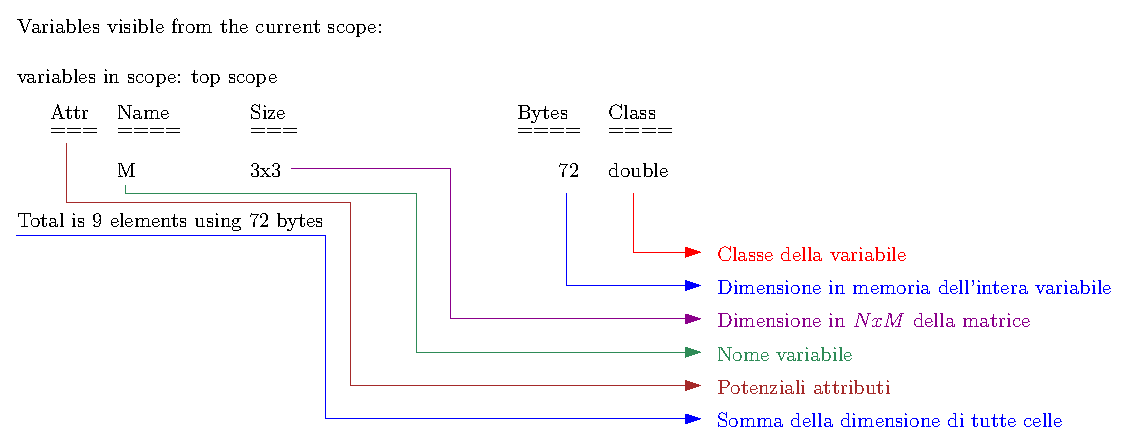
\includegraphics[width=15cm]{img/finiti/whos.eps}
  \caption{descrizione dell'interfaccia di funzione}
  \label{fig:interffun}
\end{figure}
\begin{notab}
  Anche la variabile singola viene vista come una matrice 1x1, da questo si
  denota che come il suo cugino Matlab è un software pensato per elaborare
  prodotti matriciali, infatti, il nome Matlab non sta per \texttt{Mathematic
    lab} ma per \texttt{Matrix Lab}. 
\end{notab}
\subsection{Tipi variabile}
\label{sec:tipivariabile}

\begin{table}[ht]
  \centering
  \begin{tabular}{llll}
    {\bf Nome} & {\bf Descrizione} & {\bf Dimensione} & {\bf Cifre rappresentabili}\\\hline
    \lstinline|double| ({\bf default}) & double-precision array & 8byte & $\pm1.79769x10^{308}$ a $\pm2.22507x10^{-308}$\\\hline
    \lstinline|single| & single-precision array & 4byte & $-2.1475x10^9$ a $2.1475x10^9$\\\hline 
    \lstinline|int8| & Array di interi con segno & 8bit & $-128$ a $127$\\\hline
    \lstinline|int16| & Array di interi con segno & 16bit & $-32768$ a $32767$ \\\hline
    \lstinline|int32| & Array di interi con segno & 32bit & $-2.1475x10^9$ a $2.1475x10^9$\\\hline 
    \lstinline|int64| & Array di interi con segno & 64bit & $-9.2234x10^{18}$ a $9.2234x10^{18}$\\\hline
    \lstinline|uint8| & Array di interi senza segno & 8bit & $255$\\\hline
    \lstinline|uint16| & Array di interi senza segno & 16bit & $65535$ \\\hline
    \lstinline|uint32| & Array di interi senza segno & 32bit & $4.2950x10^9$\\\hline 
    \lstinline|uint64| & Array di interi senza segno & 64bit & $1.8447x10^{19}$\\\hline
  \end{tabular}
  \caption{Tipi variabile}
  \label{tab:tipivariabile}
\end{table}
\begin{oss}
  Questa rapresentazione in memoria vale per la singola cella, quindi bisogna
  moltiplicare il paso per il numero di celle dello stesso tipo. Il programma
  peserà quanto il numero complessivo delle variabili presenti.
\end{oss}

\paragraph{Le stringhe --}
Un altro tipo di variabile però implicita sono le stringhe che il programma può
gestire, nel sequente modo \lstinline|str = "string x"| e la stampa di stringa
viene fatta con un semplice \lstinline|printf(str)|.
\clearpage
\subsubsection{Cosa stampa e cosa no}
Nel linguaggio di Matlab e Octave vengono stampate tutte le associazioni,
funzioni e inizializzazioni che non terminano con il ``{\color{red};}''.

\subsection{Impostazioni e formati}
\label{sec:formImp}
\begin{table}[ht]
  \centering
  \begin{tabular}{lll}
    {\bf Nome} & {\bf Descrizione} & {\bf Visuale}\\\hline
    \lstinline|rat| & Aspetto rateo (invece dei numeri reali rende numeri frazionari) & 1/2\\\hline
    \lstinline|short| & Formato breve a decimale fisso con 4 cifre dopo la virgola. (\textit{default}) & 0.5000\\\hline
    \lstinline|long| & Formato lungo a decimale fisso con 15 cifre dopo la virgola per & 0.500000000000000\\
                     &  i valori doppi e 7 cifre dopo la virgola per i valori singoli. \\\hline
    \lstinline|shortE| & Formato breve in annotazione scientiica con 4 cifre dopo la virgola & 5.0000e-01\\\hline
    \lstinline|longE| & Formato lungo a decimale fisso con 15 cifre dopo la virgola per & 5.000000000000000e-01\\
               & i valori doppi e 7 cifre dopo la virgola per i valori singoli.\\\hline
    \lstinline|shortG| & Formato breve, decimale fisso o notazione scientifica, a seconda & 0.5000\\
               & di quale sia più compatto, con un totale di 5 cifre.\\\hline
    \lstinline|longG| & Formato lungo a decimali fissi o notazione scientifica, qualunque & 0.500000000000000\\
               & sia il più compatto, con un totale di 15 cifre per i valori doppi e\\ & 7 cifre per i valori singoli.\\\hline
    \lstinline|shortEng| & Breve notazione ingegneristica (l'esponente è un
                           multiplo & 500.0000e-003\\
    
               &di 3) con 4 cifre dopo la virgola.\\\hline
    \lstinline|longEng| & Notazione ingegneristica lunga (l'esponente è un multiplo di 3) & 500.000000000000000e-003\\ & con 15 cifre significative.\\\hline
    \lstinline|+|&Formato positivo/negativo con caratteri +, - e vuoti visualizzati & +\\
               & per elementi positivi, negativi e zero.\\\hline
    bank & Formato valuta con 2 cifre dopo la virgola. & 0.50 \\\hline
    hex & Rappresentazione esadecimale di un numero binario & 3fe0000000000000 \\
               & a doppia precisione.\\\hline 
  \end{tabular}
  \caption{Impostazioni e formati}
  \label{tab:form}
\end{table}
\begin{notab}
  È possibile salvare il formato in una variabile con il comando \lstinline|fmt = format("nomeFormato")|
  per poi riutilizzarlo in seguito richiamando \lstinline|format(fmt)|. Altro aspetto esso può cambiare durante lo script quindi è possibile ripotare un dato
  in un formato di stampa e uno in un altro.
\end{notab}

\chapter{Proprietà delle immagini digitali}
\label{chap:propdelimmdig}

L'immagine digitale è un metodo per rappresentare di un qualcosa di
reale, e va a rappresentarlo con una matrice di pixel.

Le relazioni tra pixel (su intensità o livelli di grigio/coordinate
spaziali)
\begin{itemize}
\item misura della distanza (\textit{somiglianza}) tra i pixel;
\item vicini di un pixel; 
\item relazione di adiacenza;y
\item rapporto di connettività;
\end{itemize}
La distanza tra i punti con coordinate $(i,j)$ e $(k,l)$
\begin{itemize}
\item La distanza euclidea è definita da
  \begin{equation}
    \label{eq:propdelimmdig}
    D_E=[(i,j), (k,l)]= \sqrt{(i-k)^2+(j-l)^2}
  \end{equation}
  e la matrice risulta composta in questo modo con un $r=1$:
  \begin{equation*}
    \begin{array}[ht!]{ccccccc}
      \hline
      &&&3&&&\\
      & \sqrt{8} & \sqrt{5} & 2 & \sqrt{5} & \sqrt{8}\\
      & \sqrt{5} & \sqrt{2} & \textbf{1} & \sqrt{5} & \sqrt{2}\\
      3 & 2 & \textbf{1} & \textbf{0} & \textbf{1} & 2 & 3\\
      & \sqrt{5} & \sqrt{2} & \textbf{1} & \sqrt{5} & \sqrt{2}\\
      & \sqrt{8} & \sqrt{5} & 2 & \sqrt{5} & \sqrt{8}\\
      &&&3&&&\\\hline
    \end{array}
  \end{equation*}
\item City Block (o Manhattan)
  \begin{equation}
    \label{eq:cityblock}
    D_4[(i,j), (k,l)]=\abs{i-k}+\abs{j-l}
  \end{equation}
  e la trasposizione in matrice è la seguente con un $r=1$:
    \begin{equation*}
      \begin{array}[ht!]{ccccccc}
        \hline
        &&&3&&&\\
        &&3 & 2 & 3 &&\\
        &3& 2 & \textbf{1} & 2&3& \\
        3 & 2 & \textbf{1} & \textbf{0} & \textbf{1} & 2 & 3\\
        &3& 2 & \textbf{1} & 2&3& \\
        &&3 & 2 & 3 &&\\
        &&&3&&&\\\hline
      \end{array}
    \end{equation*}
\item Chessboard
  \begin{equation}
    \label{eq:chessboard}
    D_8=[(i,j), (k,l)]=\max\left(\abs{i-k}+\abs{j-l}\right)
  \end{equation}
  e la trasposizione in matrice è la seguente con un $r=1$:
    \begin{equation*}
    \begin{array}[ht!]{ccccccc}
      \hline
      3 & 3 & 3 & 3 & 3 & 3 & 3\\
      3 & 2 & 2 & 2 & 2 & 2 & 3\\
      3 & 2 & \textbf{1} & \textbf{1} & \textbf{1} & 2 & 3\\
      3 & 2 & \textbf{1} & \textbf{0} & \textbf{1} & 2 & 3\\
      3 & 2 & \textbf{1} & \textbf{1} & \textbf{1} & 2 & 3\\
      3 & 2 & 2 & 2 & 2 & 2 & 3\\
      3 & 3 & 3 & 3 & 3 & 3 & 3\\\hline
    \end{array}
  \end{equation*}
\item Rappresentazione di curve non semplice nel piano digitale
  \begin{itemize}
  \item Cerchio di raggio $r$, tutti i pixel che si trovano a una
    $distanza \leq r$
  \item Se $r=2$
    \begin{eqnarray*}
      \begin{array}[ht!]{ccccccc}
        \hline
        &&&3&&&\\
        & \sqrt{8} & \sqrt{5} & 2 & \sqrt{5} & \sqrt{8}\\
        & \sqrt{5} & \sqrt{2} & \textbf{1} & \sqrt{5} & \sqrt{2}\\
        3 & 2 & \textbf{1} & \textbf{0} & \textbf{1} & 2 & 3\\
        & \sqrt{5} & \sqrt{2} & \textbf{1} & \sqrt{5} & \sqrt{2}\\
        & \sqrt{8} & \sqrt{5} & 2 & \sqrt{5} & \sqrt{8}\\
        &&&3&&&\\\hline
      \end{array} &
                          \begin{array}[ht!]{ccccccc}
        \hline
        &&&3&&&\\
        &&3 & \textbf{2} & 3 &&\\
        &3& \textbf{2} & \textbf{1} & \textbf{2} & 3& \\
        3 & \textbf{2} & \textbf{1} & \textbf{0} & \textbf{1} & \textbf{2} & 3\\
        &3&\textbf{2} & \textbf{1} & \textbf{2}&3& \\
        &&3 &\textbf{2} & 3 &&\\
        &&&3&&&\\\hline
    \end{array} & \begin{array}[ht!]{ccccccc}
      \hline
      3 & 3 & 3 & 3 & 3 & 3 & 3\\
      3 & \textbf{2} & \textbf{2} & \textbf{2} & \textbf{2} & \textbf{2} & 3\\
      3 & \textbf{2} & \textbf{1} & \textbf{1} & \textbf{1} & \textbf{2} & 3\\
      3 & \textbf{2} & \textbf{1} & \textbf{0} & \textbf{1} & \textbf{2} & 3\\
      3 & \textbf{2} & \textbf{1} & \textbf{1} & \textbf{1} & \textbf{2} & 3\\
      3 & \textbf{2} & \textbf{2} & \textbf{2} & \textbf{2} & \textbf{2} & 3\\
      3 & 3 & 3 & 3 & 3 & 3 & 3\\\hline
    \end{array}
    \end{eqnarray*}
  \item Se $r=3$
    \begin{eqnarray*}
      \begin{array}[ht!]{ccccccc}
        \hline
        &&&3&&&\\
        & \sqrt{8} & \sqrt{5} & 2 & \sqrt{5} & \sqrt{8}\\
        & \sqrt{5} & \sqrt{2} & 1 & \sqrt{5} & \sqrt{2}\\
        3 & 2 & 1 & 0 & 1 & 2 & 3\\
        & \sqrt{5} & \sqrt{2} & 1 & \sqrt{5} & \sqrt{2}\\
        & \sqrt{8} & \sqrt{5} & 2 & \sqrt{5} & \sqrt{8}\\
        &&&3&&&\\\hline
      \end{array} &
                    \begin{array}[ht!]{ccccccc}
                      \hline
                      &&&3&&&\\
                      & & 3 & 2 & 3 &&\\
                      &3& 2 & 1 & 2 & 3& \\
                      3 & 2 & 1 & 0 & 1 & 2 & 3\\
                      &3& 2 & 1 & 2 &3& \\
                      &&3 & 2 & 3 &&\\
                      &&&3&&&\\\hline
                    \end{array} & \begin{array}[ht!]{ccccccc}
                      \hline
                      3 & 3 & 3 & 3 & 3 & 3 & 3\\
                      3 & 2 & 2 & 2 & 2 & 2 & 3\\
                      3 & 2 & 1 & 1 & 1 & 2 & 3\\
                      3 & 2 & 1 & 0 & 1 & 2 & 3\\
                      3 & 2 & 1 & 1 & 1 & 2 & 3\\
                      3 & 2 & 2 & 2 & 2 & 2 & 3\\
                      3 & 3 & 3 & 3 & 3 & 3 & 3\\\hline
                    \end{array}
    \end{eqnarray*}
  \end{itemize}
\end{itemize}
\begin{nota}
  Nel ultimo caso tutta l'aria disponibile è selezionata.
\end{nota}

\section{Neighborhood}
\label{sec:neiborhood}

\begin{defi}
  Il Neighborhood (l'intorno) sono quelle tecniche di elaborazione delle
  immagini in cui il valore risultante per un pixel alle coordinate
  $(x_1,y_1)$ -- è una funzione del valore del pixel originale in quel
  punto così come del valore del pixel originale di alcuni dei suoi
  vicinato. Il modo in cui i valori l'intorno e il valore del pixel di
  riferimento vengono combinati per produrre il risultato può variare
  in modo significativo tra i diversi algoritmi.
\end{defi}
\clearpage
\begin{itemize}
\item Proprietà locali per ogni due pixel
  \begin{itemize}
  \item 4-neighbors (\texttt{4 pixel vicini});
    \begin{itemize}
    \item $D_4 = 1$ (Distanza d'intorno);
    \item $(i+1, j), (i-1, j), (i, j+1), (i, j-1)$
    \end{itemize}
  \item Pixel adiacenti a $(i, j)$:
    \begin{figure}[ht!]
      \centering
      % author: Nicola Ferru <ask dot nfvblog at outlook dot it>

\begin{tikzpicture}
	\draw (-1,0) -- (0,0) -- (0,1) -- (1,1) -- (1,0) -- (2,0) -- (2,-1) -- (1,-1) -- (1,-2) -- (0,-2) -- (0,-1) -- (-1,-1) -- cycle;
	\draw[fill] (0,0) -- (0,-1) -- (1,-1) -- (1,0) -- cycle;
\end{tikzpicture}
      \caption{Intorno 4-neighbors}
      \label{fig:4-neigh}
    \end{figure}
  \item 8-neighbors (\texttt{8 pixel vicini});
    \begin{itemize}
    \item $D_8 = 1$ (Distanza d'intorno);
    \item $(i+1, j), (i-1, j), (i, j+1), (i, j-1), (i+1, j+1),
      (i+1, j-1), (i-1, j+1), (i-1, j-1)$
    \end{itemize}
  \item Pixel adiacenti a $(i, j)$:
    \begin{figure}[ht!]
      \centering
      % author: Nicola Ferru <ask dot nfvblog at outlook dot it>

\begin{tikzpicture}
	% bordo esterno
	\draw (-1,0) -- (-1,1) -- (0,1);
	\draw (1,1) -- (2,1) -- (2,0);
	\draw (2,-1) -- (2,-2) -- (1,-2);
	\draw (-1,-1) -- (-1,-2) -- (1,-2);
	% bordo interno +
	\draw (-1,0) -- (0,0) -- (0,1) -- (1,1) -- (1,0) -- (2,0) -- (2,-1) -- (1,-1) -- (1,-2) -- (0,-2) -- (0,-1) -- (-1,-1) -- cycle;
	\draw[fill] (0,0) -- (0,-1) -- (1,-1) -- (1,0) -- cycle;
\end{tikzpicture}
      \caption{Intorno 8-neighbors}
      \label{fig:8-neigh}
    \end{figure}    
  \end{itemize}
\end{itemize}

\subsection{Adjacency (Adiacenza)}
\label{sec:adjacency}

Strettamente legato al concetto di vicinato: due pixel si dicono
adiacenti se esistono vicini (\emph{o meglio vicini}) tali che i loro
valori di intensità soddisfano alcuni specifici criteri di similarità.
\begin{itemize}
\item Adiacenza tra i pixel:
  \begin{itemize}
  \item Un insieme di pixel è connesso se sono adiacenti
  \item Sono adiacenti se la loro distanza è uguale a 1
    \begin{itemize}
    \item 4-adiacenza quando $D_4 = 1$
    \item 8-adiacenza quando $D_8 = 1$
    \end{itemize}
  \end{itemize}
\end{itemize}

\subsection{Path between pixels}
\label{sec:pathbetpixels}

Prendendo 2 pixel (A,B) è possibile stimare una distanza, quella è la
path:
\begin{itemize}
\item La sequenza di pixel distinti $S_i$ con $i =1,\dots,n$
\item Dove:
  \begin{itemize}
  \item $S_1 = A$ e $S_n = B$
  \item $S_i$ e $S_{i-1}$ sono adiacenti per $1\leq i\leq n$
  \end{itemize}
  \begin{figure}[ht!]
    \centering
    \resizebox{8cm}{!}{
    % Author: Nicola Ferru <ask dot nfvblog at outlook dot it>
\begin{tikzpicture}
	\draw[step=1.0,black,thin] (0.5,0.5) grid (13.5,13.5);
	\draw[fill] (3,3) -- (4,3) -- (4,5) -- (8,5) -- (8,8) -- (9,8) -- (9,12) -- (8,12) -- (8,9) -- (7,9) -- (7,6) -- (3,6)-- cycle;
	\node at (8.5,12.5) {B};
	\node at (3.5,2.5) {A};
	\draw[step=1.0,black,thin] (14.5,0.5) grid (28.5,13.5);
	\draw[fill] (16,3) -- (17,3) -- (17,7) -- (18,7) -- (18,10) -- (23,10) -- (23, 8) -- (24,8) -- (24, 10) -- (23, 10) -- (23,11) -- (18,11) -- (18,10) -- (17,10)
		-- (17,7) -- (16,7);
 	\node at (23.5,7.5) {B};
	\node at (16.5,2.5) {A};
	\node at (6.5, 0) {{\Large 4-path}};
	\node at (22, 0) {{\Large 8-path}};
\end{tikzpicture}}
    \caption{Patch between pixels}
    \label{fig:pathpix}
  \end{figure}
\item Percorso chiuso
  \begin{itemize}
  \item Se il primo e l'ultimo pixel sono vicini
  \end{itemize}
\item Ambiguità nelle curve chiuse
  \begin{itemize}
  \item Nel piano reale una curva divide l'interno e l'esterno
  \item Nel piano digitale esiste tale separazione!?
  \end{itemize}
  \begin{figure}[ht!]
    \centering
    \resizebox{8cm}{!}{
    \begin{tikzpicture}
	\draw[step=1.0,black,thin] (0.5,0.5) grid (13.5,13.5);
	\draw[step=1.0,black,thin] (14.5,0.5) grid (27.5,13.5);
	\draw[fill] (5,10) -- (9,10) -- (9,9) -- (5,9);
	\draw[fill] (9,9) -- (10,9) -- (10,5) -- (9,5);
	\draw[fill] (5,5) -- (9,5) -- (9,4) -- (5,4);
	\draw[fill] (4,9) -- (5,9) -- (5,5) -- (4,5);
	\draw[fill] (19,10) -- (23,10) -- (23,9) -- (19,9);
	\draw[fill] (19,10) -- (18,10) -- (18,5) -- (19,5);
	\draw[fill] (18,5) -- (18,4) -- (23,4) -- (23,5);
	\draw[fill] (23,10) -- (24,10) -- (24,4) -- (23,4);

\end{tikzpicture}}
    \caption{Patch between pixels curva chiuse}
    \label{fig:pathpix2}
  \end{figure}
\end{itemize}

\subsection{Connectivity}
\label{sec:conct}
\begin{itemize}
\item Due pixel $A$ e $B$ sono collegati se c'è un percorso tra di loro.
\item Dati i pixel $A$, $B$ e $C$
  \begin{itemize}
  \item \textbf{Riflessività}: $A$ è collegato ad $A$
  \item \textbf{Commutatività}: se $A$ è connesso a $B$ allora $B$ è
    connesso ad $A$
  \item \textbf{Transitivity}: if $A$ is connected to $B$ and $B$ is
    connected to $C$ then $A$ is connected to $C$
  \end{itemize}
\end{itemize}

\subsection{Region}
\label{sec:region}

\begin{defi}
  La regione dell'immagine è un metodo in cui un'immagine digitale viene
  suddivisa in vari sottogruppi chiamati segmenti di immagine, che
  aiutano a ridurre la complessità dell'immagine per semplificarne
  l'elaborazione o l'analisi. In altre parole, la segmentazione implica
  l'assegnazione di etichette ai pixel. A tutti gli elementi
  dell'immagine o ai pixel appartenenti alla stessa categoria è
  assegnata un'etichetta comune.
\end{defi}

\subsection{Edge}
\label{sec:edge}
\begin{figure}[ht!]
  \centering
  \resizebox{5cm}{!}{
    \begin{tikzpicture}
	\draw[step=1.0,black,thin] (0.5,0.5) grid (8.5,8.5);
	\draw[fill,opacity=0.8] (0.5,6) -- (3,6) -- (3,5) -- (5,5) -- (5,4) -- (7,4) -- (7,3) -- (8.5,3) -- (8.5,0.5) -- (0.5,0.5)-- cycle;
\end{tikzpicture}}
  \caption{Edge}
  \label{fig:edge}
\end{figure}
Edge è una proprietà locale di un pixel e delle sue immediate vicinanze;
mentre il confine è un concetto globale associato ad una regione e
forma un percorso chiuso, il bordo esprime le proprietà locali di una
funzione immagine:
\begin{itemize}
\item Tutti i pixel del bordo sono anche bordi
\end{itemize}
I bordi sono importanti per il sistema visivo umano, poiché costituiscono informazioni di base per il riconoscimento
\begin{itemize}
\item Punti di cambiamento improvviso dei livelli di grigio, discontinuità di intensità
\end{itemize}

\subsection{Convex hull}
\label{sec:convex}
Il convex hull è la regione più piccola che contiene l'oggetto, in
modo tale che due punti qualsiasi della regione possono essere collegati
da una linea retta, tutti i punti della quale appartengono alla regione.
\begin{figure}[ht!]
  \centering
  \resizebox{5cm}{!}{
    \begin{tikzpicture}
	\draw[step=1.0,black,thin] (0.5,0.5) grid (8.5,8.5);
	\draw[fill] (2,7) --(3,7) --(3,5) -- (7,5) -- (7,4) -- (3,4) -- (3,1) -- (2,1);
	\draw[fill] (3,7) -- (3,8) -- (7,8) -- (7,7) -- (8,7) -- (8,5) -- (7,5) -- (7,7);
	\draw[fill] (4,4) -- (5,4) -- (5,3) -- (6,3) -- (6,2) -- (7,2) -- (7,1) -- (6,1) -- (6,2) -- (5,2) -- (5,3) -- (4,3);
\end{tikzpicture}}
  \caption{Convex hull}
  \label{fig:convex}
\end{figure}

\subsection{Area, perimetro}
\label{sec:areaeper}

\begin{itemize}
\item L'\textbf{Area} è la somma dei pixel dell'oggetto.
\item Il \textbf{Perimetro} è la somma dei pixel appartenenti al confine
\end{itemize}
\clearpage
\begin{figure}[ht!]
  \centering
  \resizebox{10cm}{!}{
    \begin{tikzpicture}
	\draw[step=1.0,black,thin] (0.5,0.5) grid (8.5,8.5);
	\draw[red, fill, opacity=0.8] (1,2) -- (2,2) -- (2,1) -- (7,1) -- (7,2) -- (8,2) -- (8,4) -- (7,4) -- (7,5) -- (6,5) -- (6,6) -- (3,6) -- (3,5) -- (2,5) -- (2,4) -- (1,4) -- cycle;
	\draw[fill] (2,2) -- (7,2) -- (7,4) -- (6,4) -- (6,5) -- (3,5) -- (3,4) -- (2,4);
	\draw[step=1.0,black,thin] (9.5,0.5) grid (16.5,8.5);
	\draw [fill,red, opacity=0.8] (10,7) -- (16,7) -- (16,5) -- (14,5) -- (14,) -- (12,) -- (12,5) -- (10,5);
	\node  at (4.5,-0.5) {$Area = 22$};
	\node at (4.5,-1) {$Perimeter = 12$};
	\node  at (13,-0.5) {$Area = 20$};
	\node at (13,-1) {$Perimeter = 22$};	
\end{tikzpicture}}
  \caption{Area e perimetro}
  \label{fig:areaper}
\end{figure}

\subsection{Tipologia di operazioni}
\label{sec:tipop}
There is a variety of ways to classify and characterize image operations
\begin{itemize}
\item In base alla relazione input/output
\item In base al risultato atteso di questa operazione
\item In base al tipo di operazione 
\item In base al costo di tale operazione 
\item In base al dominio di applicazione
\end{itemize}
Generalmente le operazioni sono classificate come \textbf{puntuali},
\textbf{locali} o \textbf{globali}. Il valore di uscita ad una
coordinata specifica dipende:

\begin{itemize}
\item \textbf{Punto}: solo sul valore di input alla stessa coordinata.
\item \textbf{Locale}: sui valori di input nell'intorno di quella stessa
  coordinata. 
\item \textbf{Globale}: su tutti i valori nell'immagine di input.
\end{itemize}

\subsubsection{Operazioni a punto}
\label{sec:opapunto}

Il valore di output su una coordinata specifica dipende solo dal valore di input su quella stessa coordinata
\begin{itemize}
\item tipicamente si tratta di operazioni elementari su ciascun pixel
\item pertanto possono includere solo trasformazioni di intensità
\end{itemize}
Un esempio di questo tipo di operazioni è proprio il negativo di
immagine.
\section{Creazione di una immagine digitale}
\label{sec:creadiunimgdig}

\begin{description}
\item[Sampling] il processo che consiste nella downscaling dell'immagine
  o nella rimozione di pixel (\textit{pratica che fa pardere
    delle info});
  \begin{itemize}
  \item \textit{Lineare}: va a scalare tutta l'area dell'immagine in
    modo lineare e uniforme.
  \item \textit{Adattivo}: va a fare uno sampling in base all'importanza
    delle aree.
  \end{itemize}
\item[Quantizzazione] il processo che che va a motificare la profondità
  del colore
  \begin{itemize}
  \item Viene utilizzato per l'analisi dell'immagine e anche per le
    immagini personali.
  \item Problemi da risolvere: Memorizzazione e trasferimento.
  \end{itemize}
\end{description}
E su questi principi sono la base dell'elaborazione dell'immagine
digitale e del campionamento.

\subsection{Tipo di immagine}
\label{sec:tipodiimm}
\begin{itemize}
\item Numero di livello di intensità;
\item Numero di piani dell'immagine:
  \begin{itemize}
  \item Immagine binaria: è un immagine composta unicamente da bianco e
    nero;
  \item A livelli di grigio: è un'immagine che funziona a sfumature di
    grigio;
  \item A colori: sono composte da sfumature RGB che vanno da 0 a 255
    per creare una paletta cromatica accettabile (\ref{sec:raster}).
  \end{itemize}
\end{itemize}
Per generare le tipoligie di immagini si utilizzano dei canali:
\begin{table}[ht!]
  \centering
  \begin{tabular}{lrc}
    \textbf{Tipologie}&\textbf{Numero di canali}& \textbf{Dimensione}
    \\\hline
    bianco e nero & 1 &(1bit)\\
    Immagini a livelli di grigio & 1 &(8bit)\\
    Immagini a colori & 3 &(8bit)\\\hline
  \end{tabular}
  
  \caption{Numero di canali per le tipoligie di immagine}
  \label{tab:numcanimg}
\end{table}

\subsection{Rappresentazione di immagine}
\label{sec:raprimg}
\begin{itemize}
\item \textbf{Iconic Images}: Immagini che contengono i dati originali
  con l'intensità dei singoli pixel;
\item \textbf{Segmented images}: Immagini in cui i pixel sono divisi in
  gruppi in base all'appartenenza o meno agli oggetti;
\item \textbf{Geometric representations}: conoscenza attuale delle forme;
\item \textbf{Relational models}: presentare la conoscenza sugli oggetti
  e sulle relazioni con altri oggetti nell'immagine.
\end{itemize}

\section{Strutture dati}
\label{sec:strutdati}
Le strutture dati, sono le entità matematiche che consentono di
ragruppare più di un valore all'interno dello stesso insieme, per poter
più facilmente gestire, ordinare, ed elaborare il contenuto. Cosa
non possibile con variabili primitive\footnote{È una variabile che può
  contenere solo una tipologia singolarmente, da esse si possono
  creare le così dette \lstinline|struct| e anche delle strutture dati.}.
\subsection{Matrice}
\label{sec:matrice}
\begin{itemize}
\item La struttura dati più comune per rappresentare le immagini;
\item Gli elementi dell'array sono numeri interi;
\item Le caratteristiche spaziali sono implicitamente disponibili.
\end{itemize}
\begin{equation}
  \label{eq:matrice}
  \begin{array}{c|ccccccc}
      & 1 & 2 & 3 & 4 & 5 & 6 & 7 \\\hline
    1 & 1 & 2 & 1 & 3 & 1 & 1 & 1 \\
    2 & 2 & 1 & 1 & 1 & 2 & 3 & 4 \\
    3 & 1 & 2 & 1 & 1 & 1 & 1 & 4 \\
    4 & 1 & 2 & 2 & 2 & 1 & 3 & 1 \\
    5 & 1 & 2 & 2 & 2 & 1 & 1 & 4 \\
    6 & 2 & 2 & 2 & 1 & 1 & 1 & 1 \\
    7 & 1 & 4 & 1 & 1 & 1 & 1 & 1
  \end{array}
\end{equation}

\subsection{Vettore}
\label{sec:vettore}

\begin{itemize}
\item Molto comune per estrarre e archiviare informazioni dall'immagine;
\item Gli esempi di array sono in genere numeri interi;
\item Anche in questo caso il suo contenuto è accessibile attraverso
  informazioni implicite;
\item Gli array non sono altro che array bidimensionali.
\end{itemize}
\begin{equation}
  \label{eq:vettore}
  \begin{array}{ccccc}
    0&1&2&3&4\\\hline
    2&2&1&1&4\\\hline
  \end{array}
\end{equation}
\begin{nota}
  A lato logico all'interno di quasi tutti i linguaggi di
  programmazione, sia i vettori che le matrici fanno parte dello stesso
  tipo di struttura dati, i così detti Array, che possono avere
  \texttt{N} dimensioni. Tipicamente per scorrere suddette strutture si
  utilizzano delle variabili definite ``contatori'', indicate con le
  lettere: \texttt{i,j,k,h} assegnate per comodità visto che stanno in
  un area della tastiera vicina al posizionamento delle mani.
\end{nota}

\subsection{Topologie}
\label{sec:topologie}
Sono una categoria di strutture dati che possono servire ad indicare
logicamente le relazioni. Esse vengono utilizzate anche nel ambito
del processing delle immagini per distrivere le singole relazioni,
ne esistono di diversa tipologie:
\begin{itemize}
\item Grafo: tipologia ad albero utilizzato in tutto quello che prevede
  stati o connessioni;
\item Insiemi: permettono di stabilire appertenenze a ordini gerarchici.
\end{itemize}
\begin{figure}[ht!]
  \centering
  \def\b{.3}
\def\cr{.53}
\begin{tikzpicture} 
%\draw (1.5,1.5) circle [radius=\cr];
\node at (1.5,4.5) {$N= ?$ $R=?$};
% centro a maglia
\draw (1.5,1) circle [radius=\b];
\draw (1,1.9) circle [radius=\b];
\draw (2,1.9) circle [radius=\b];
\draw (2,1.9) -- (1,1.9) -- (1.5,1) -- (2,1.9);
% end centro 

\draw (1.5,1) -- (0,0);
\draw (0,0) circle [radius=\b];

\draw (1.5,1) -- (1.5,0);
\draw (1.5,0) circle [radius=\b];

\draw (3,0) -- (1.5,1);
\draw (3,0) circle [radius=\b];

\draw (1,1.9) -- (0,3);
\draw (0,3) circle [radius=\b];

\draw (2,1.9) -- (3,3);
\draw (3,3) circle [radius=\b];

\draw (2,1.9) -- (2.5,3.7);
\draw (2.5,3.7) circle [radius=\b];
\end{tikzpicture}
  \caption{Grafo}
  \label{fig:grafo}
\end{figure}
Mentre, nel caso dell'insieme la situazione è la seguente:
\begin{figure}[ht!]
  \centering
  \resizebox{8cm}{!}{
  \newcommand{\boundellipse}[3]% center, xdim, ydim
{(#1) ellipse (#2 and #3)
}

\begin{tikzpicture}
	\draw [draw=black] (-6,-5) rectangle  (6,4);
	\node at (-5,3.4){1};
	\draw \boundellipse{2,0}{1}{2};
	\draw \boundellipse{0,0}{5}{3};
	\draw (-4,-1.8) arc (-35:37.7:3);
	\node at (-4,1) {3};
	\node at (0.4,2){4};
	\node at (2,1)  {5};
	\node at (2.5,4.5)  {0};
	\draw (4,4) arc (-180:-90.7:2);
	\node at (5.5,3.5){2};
\end{tikzpicture}
}
  \caption{Insieme}
  \label{fig:insieme}
\end{figure}
\begin{nota}
  In entrambi i casi, la situazione è molto leggibile e si capisce
  anche la relazione in base al livello oppure al sotto insieme a cui
  il valore appartiene.
\end{nota}

\subsection{Gerarchico}
\label{sec:hierarchical}
\begin{itemize}
\item Sono nati per alleggerire il calcolo di operazioni molto complesse,
  ad esempio suddividendo i calcoli tra più computer;
\item Dividendo l'immagine in blocchi
\item Spesso non è così semplice dividere i compiti tra più computer
\item Le informazioni presenti in un blocco possono essere utili per
  elaborare quello adiacente
\item Non tutti i blocchi immagine devono essere elaborati allo stesso
  modo
\end{itemize}

\subsection{Piramidale (pyramids)}
\label{sec:pyramid}

\subsubsection{M-pyramids}
\label{sec:mpyram}
\begin{itemize}
\item Sono una sequenza di immagini con risoluzioni diverse;
\item Utilizzato quando è necessario lavorare con risoluzioni diverse
  contemporaneamente
\item Ovviamente un array di grado inferiore contiene 4 volte meno dati
  e può essere elaborato circa 4 volte più velocemente
\end{itemize}
Ed esempio, è possibile vedere come nella matrice $I_3$ sia una matrice
8x8, mentre, la matrice $I_2$ è una matrice 4x4, nella matrice $I_1$ è
un 2x2 e $I_0$ è una cella singola. 
\begin{eqnarray}
  \label{eq:mpyram}
  I_3=
  \begin{pmatrix}
    2 & 4 & 8 & 0 & 0 & 2 & 6 & 3\\
    3 & 0 & 0 & 1 & 1 & 3 & 6 & 4\\
    2 & 2 & 0 & 1 & 1 & 4 & 6 & 3\\
    3 & 2 & 1 & 1 & 1 & 2 & 6 & 3\\
    4 & 3 & 1 & 1 & 2 & 3 & 6 & 3\\
    4 & 4 & 2 & 1 & 2 & 4 & 7 & 5\\
    5 & 4 & 2 & 1 & 1 & 4 & 7 & 5\\
    5 & 5 & 1 & 0 & 0 & 2 & 7 & 5
  \end{pmatrix} &
  I_2=\begin{pmatrix}
    2 & 2 & 2 & 5\\
    2 & 1 & 2 & 5\\
    4 & 1 & 3 & 5\\
    5 & 1 & 2 & 6
  \end{pmatrix} & I_1=
  \begin{pmatrix}
    2 & 4\\
    3 & 4
  \end{pmatrix} I_0=
  \begin{pmatrix}
    3
  \end{pmatrix}
\end{eqnarray}
\begin{nota}
  Il rapporto tra un immagine e l'altra è un rapporto ad esponenziale di
  con base 2, infatti $I_3$ è un $2^3$, mentre, $I_0$ è un $2^0$. 
\end{nota}
\subsubsection{T-Pyramid}
\label{sec:treepy}
\begin{figure}[ht!]
  \centering
  \resizebox{15cm}{!}{
  \usetikzlibrary{graphs}

% Node styles
\tikzset{
% Two node styles for game trees: solid and hollow
solid node/.style={circle,draw,inner sep=1.5,fill=black},
hollow node/.style={circle,draw,inner sep=1.5}
}

\begin{tikzpicture} [scale=1,font=\footnotesize]
\tikzstyle{level 1}=[sibling distance=50mm] 
\tikzstyle{level 2}=[sibling distance=25mm] 
\tikzstyle{level 3}=[sibling distance=6mm] 
%radice
\node(0)[solid node]{}
% braccio destro
child{ node(1)[solid node][left]{}
child{ node(2)[solid node][left]{}
child{node(17)[solid node][left]{}}
child{node(18)[solid node][left]{}}
child{ node(3)[solid node][right]{}
edge from parent node[left]{livello 2}}
child{ node(12)[solid node][left]{}}
edge from parent node[left]{Livello 1}}
child{ node(4)[solid node][right]{}
child{node(10)[solid node][left]{}}
child{node(11)[solid node][left]{}}
child{node(15)[solid node][right]{}}
child{node(16)[solid node][right]{}}}
edge from parent node[left]{Livello 0}}
% braccio sinistro 2
child{ node(34)[solid node][right]{} 
child {node(35)[solid node][left]{}
child{node(36)[solid node][left]{}}
child{node(37)[solid node][left]{}}
child{node(38)[solid node][right]{}}
child{node(39)[solid node][right]{}}}
child{node(40)[solid node][left]{}
child{node(41)[solid node][left]{}}
child{node(42)[solid node][left]{}}
child{node(43)[solid node][right]{}}
child{node(44)[solid node][right]{}}}}
% braccio destro
child{ node(5)[solid node][right]{} 
child {node(6)[solid node][left]{}
child{node(7)[solid node][left]{}}
child{node(8)[solid node][left]{}}
child{node(19)[solid node][right]{}}
child{node(20)[solid node][right]{}}}
child{node(9)[solid node][left]{}
child{node(13)[solid node][left]{}}
child{node(14)[solid node][left]{}}
child{node(21)[solid node][right]{}}
child{node(22)[solid node][right]{}}}}
% braccio destro 2
child{ node(23)[solid node][right]{} 
child {node(24)[solid node][left]{}
child{node(25)[solid node][left]{}}
child{node(26)[solid node][left]{}}
child{node(27)[solid node][right]{}}
child{node(28)[solid node][right]{}}}
child{node(29)[solid node][left]{}
child{node(30)[solid node][left]{}}
child{node(31)[solid node][left]{}}
child{node(32)[solid node][right]{}}
child{node(33)[solid node][right]{}}}};

\end{tikzpicture}}
  \caption{Esempio di albero piramidale}
  \label{fig:alberopir}
\end{figure}
Da questo grafico è possibile dedurre che:
\begin{itemize}
\item Viene utilizzato per dividere gerarchicamente l'immagine in regioni
  adiacenti;
\item Queste regioni possono essere rappresentate da un albero;
\item Ogni nodo di questo albero ha 4 figli.
\end{itemize}

\subsubsection{Quad-tree}
\label{sec:quad-tree}
\begin{figure}[ht!]
  \centering
  \usetikzlibrary{graphs}

% Node styles
\tikzset{
% Two node styles for game trees: solid and hollow
solid node/.style={circle,draw,inner sep=2,fill=black},
hollow node/.style={circle,draw,inner sep=2},
rect hollow node/.style={rectangle,draw,inner sep=2},
rect solid node/.style={rectangle,draw, inner sep=2, fill=gray}
}

\begin{tikzpicture} [scale=1,font=\footnotesize]
\draw (0,2) -- (4,2);
\draw (2,0) -- (2,4);
\draw (2,1) -- (4,1);
\draw (3,0) -- (3,4);
\draw (0,3) -- (4,3);
\draw (1,2) -- (1,4);
\draw (1,2) -- (1,4);
\draw (1.5,3) -- (1.5,4);
\draw (2,3.5) -- (1,3.5);

\draw[brown, very thick] (0,0) rectangle (4,4);
\draw node[rect solid node] at (1.75,3.74) {E};
\draw node[rect solid node] at (1.25,3.25) {C};
\draw node[rect solid node] at (2.5,2.5) {A};
\draw node[rect solid node] at (3.5,1.5) {B};
\draw node[rect solid node] at (2.5,0.5) {D};
\end{tikzpicture}
  \caption{Quad-tree}
  \label{fig:qtree1}
\end{figure}
In questo modello partiamo da una rappresentazione inscritta in un
quadrato, che contiene al suo interno determinati valori, più il valore
è contenuto all'interno di un sotto quadrato più sarà in un livello
superiore\footnote{Gli alberi si leggono dall'alto verso il basso, quindi
  il livello sarà più alto più sarà in basso.}.
\begin{figure}[ht!]
  \centering
  \usetikzlibrary{graphs}

% Node styles
\tikzset{
% Two node styles for game trees: solid and hollow
solid node/.style={circle,draw,inner sep=2,fill=black},
hollow node/.style={circle,draw,inner sep=2},
rect hollow node/.style={rectangle,draw,inner sep=2},
rect solid node/.style={rectangle,draw, inner sep=2, fill=gray}
}

\begin{tikzpicture} [scale=1,font=\footnotesize]
\tikzstyle{level 1}=[sibling distance=25mm] 
\tikzstyle{level 2}=[sibling distance=7mm] 
\tikzstyle{level 3}=[sibling distance=6mm] 
%radice
\node(0)[hollow node]{}
child{node(1)[hollow node]{}
child{node(9)[rect hollow node]{}}
child{node(10)[hollow node]{}
child{node(13)[rect hollow node]{}}
child{node(14)[rect solid node]{E}}
child{node(15)[rect solid node]{C}}
child{node(16)[rect hollow node]{}}}
child{node(17)[rect hollow node]{}}
child{node(12)[rect hollow node]{}}
}
child{node(2)[hollow node]{}
child{node(5)[rect hollow node]{}}
child{node(6)[rect hollow node]{}}
child{node(7)[rect solid node]{A}}
child{node(8)[rect hollow node]{}}}
child{node(3)[rect hollow node]{}}
child{node(4)[hollow node]{}
child{node(14)[rect hollow node]{}}
child{node(15)[rect solid node]{B}}
child{node(16)[rect hollow node]{}}
child{node(17)[rect solid node]{D}}};

\end{tikzpicture}
  \caption{Quad-tree}
  \label{fig:qtree2}
\end{figure}
\begin{itemize}
\item Deriva da una modifica della T-pyramid
\item Non crea figli per ogni nodo ma solo quando i figli sono diversi
\end{itemize}
\clearpage
\subsection{Histogram (Istogramma)}
\label{sec:histogram}
L'istogramma nel processo di elaborazione dell'immagine, viene utilizzato
per verificare la presenta delle corrispettive tonalità di colore e
anche la sua frequenza o di scale di grigio in base alla situazione.
Un altro caso di utilizzo è la verifica del contrasto\footnote{Il
  contrasto è la differenza tra una porzioni d'immagine e il suo
sfondo, più esso è altro maggiore la parte in questione sarà risaltata}
di una immagine. Ad esempio, prendedo la foto di un gatto:
\begin{figure}[ht!]
  \centering
  \includegraphics[height=3cm]{img/gatto.jpg}
  \caption{Gatto}
  \label{fig:gatto}
\end{figure}

Il suo istogramma sarà composto, nel seguente modo, ricordano che la
gamma dei colori va da 0 a 255 come espresso in (\ref{sec:rgbcolor}),
la scala del grafico sarà proprio quella.
\begin{figure}[ht!]
  \centering
  \resizebox{15cm}{!}{
  %% Creator: Matplotlib, PGF backend
%%
%% To include the figure in your LaTeX document, write
%%   \input{<filename>.pgf}
%%
%% Make sure the required packages are loaded in your preamble
%%   \usepackage{pgf}
%%
%% Also ensure that all the required font packages are loaded; for instance,
%% the lmodern package is sometimes necessary when using math font.
%%   \usepackage{lmodern}
%%
%% Figures using additional raster images can only be included by \input if
%% they are in the same directory as the main LaTeX file. For loading figures
%% from other directories you can use the `import` package
%%   \usepackage{import}
%%
%% and then include the figures with
%%   \import{<path to file>}{<filename>.pgf}
%%
%% Matplotlib used the following preamble
%%   
%%   \usepackage{fontspec}
%%   \setmainfont{DejaVuSerif.ttf}[Path=\detokenize{/usr/share/matplotlib/mpl-data/fonts/ttf/}]
%%   \setsansfont{DejaVuSans.ttf}[Path=\detokenize{/usr/share/matplotlib/mpl-data/fonts/ttf/}]
%%   \setmonofont{DejaVuSansMono.ttf}[Path=\detokenize{/usr/share/matplotlib/mpl-data/fonts/ttf/}]
%%   \makeatletter\@ifpackageloaded{underscore}{}{\usepackage[strings]{underscore}}\makeatother
%%
\begingroup%
\makeatletter%
\begin{pgfpicture}%
\pgfpathrectangle{\pgfpointorigin}{\pgfqpoint{13.620000in}{6.720000in}}%
\pgfusepath{use as bounding box, clip}%
\begin{pgfscope}%
\pgfsetbuttcap%
\pgfsetmiterjoin%
\definecolor{currentfill}{rgb}{1.000000,1.000000,1.000000}%
\pgfsetfillcolor{currentfill}%
\pgfsetlinewidth{0.000000pt}%
\definecolor{currentstroke}{rgb}{1.000000,1.000000,1.000000}%
\pgfsetstrokecolor{currentstroke}%
\pgfsetdash{}{0pt}%
\pgfpathmoveto{\pgfqpoint{0.000000in}{0.000000in}}%
\pgfpathlineto{\pgfqpoint{13.620000in}{0.000000in}}%
\pgfpathlineto{\pgfqpoint{13.620000in}{6.720000in}}%
\pgfpathlineto{\pgfqpoint{0.000000in}{6.720000in}}%
\pgfpathlineto{\pgfqpoint{0.000000in}{0.000000in}}%
\pgfpathclose%
\pgfusepath{fill}%
\end{pgfscope}%
\begin{pgfscope}%
\pgfsetbuttcap%
\pgfsetmiterjoin%
\definecolor{currentfill}{rgb}{1.000000,1.000000,1.000000}%
\pgfsetfillcolor{currentfill}%
\pgfsetlinewidth{0.000000pt}%
\definecolor{currentstroke}{rgb}{0.000000,0.000000,0.000000}%
\pgfsetstrokecolor{currentstroke}%
\pgfsetstrokeopacity{0.000000}%
\pgfsetdash{}{0pt}%
\pgfpathmoveto{\pgfqpoint{1.702500in}{0.739200in}}%
\pgfpathlineto{\pgfqpoint{12.258000in}{0.739200in}}%
\pgfpathlineto{\pgfqpoint{12.258000in}{5.913600in}}%
\pgfpathlineto{\pgfqpoint{1.702500in}{5.913600in}}%
\pgfpathlineto{\pgfqpoint{1.702500in}{0.739200in}}%
\pgfpathclose%
\pgfusepath{fill}%
\end{pgfscope}%
\begin{pgfscope}%
\pgfpathrectangle{\pgfqpoint{1.702500in}{0.739200in}}{\pgfqpoint{10.555500in}{5.174400in}}%
\pgfusepath{clip}%
\pgfsetbuttcap%
\pgfsetmiterjoin%
\definecolor{currentfill}{rgb}{0.121569,0.466667,0.705882}%
\pgfsetfillcolor{currentfill}%
\pgfsetlinewidth{0.000000pt}%
\definecolor{currentstroke}{rgb}{0.000000,0.000000,0.000000}%
\pgfsetstrokecolor{currentstroke}%
\pgfsetstrokeopacity{0.000000}%
\pgfsetdash{}{0pt}%
\pgfpathmoveto{\pgfqpoint{1.702500in}{0.739200in}}%
\pgfpathlineto{\pgfqpoint{1.743894in}{0.739200in}}%
\pgfpathlineto{\pgfqpoint{1.743894in}{0.808931in}}%
\pgfpathlineto{\pgfqpoint{1.702500in}{0.808931in}}%
\pgfpathlineto{\pgfqpoint{1.702500in}{0.739200in}}%
\pgfpathclose%
\pgfusepath{fill}%
\end{pgfscope}%
\begin{pgfscope}%
\pgfpathrectangle{\pgfqpoint{1.702500in}{0.739200in}}{\pgfqpoint{10.555500in}{5.174400in}}%
\pgfusepath{clip}%
\pgfsetbuttcap%
\pgfsetmiterjoin%
\definecolor{currentfill}{rgb}{0.121569,0.466667,0.705882}%
\pgfsetfillcolor{currentfill}%
\pgfsetlinewidth{0.000000pt}%
\definecolor{currentstroke}{rgb}{0.000000,0.000000,0.000000}%
\pgfsetstrokecolor{currentstroke}%
\pgfsetstrokeopacity{0.000000}%
\pgfsetdash{}{0pt}%
\pgfpathmoveto{\pgfqpoint{1.743894in}{0.739200in}}%
\pgfpathlineto{\pgfqpoint{1.785288in}{0.739200in}}%
\pgfpathlineto{\pgfqpoint{1.785288in}{0.851602in}}%
\pgfpathlineto{\pgfqpoint{1.743894in}{0.851602in}}%
\pgfpathlineto{\pgfqpoint{1.743894in}{0.739200in}}%
\pgfpathclose%
\pgfusepath{fill}%
\end{pgfscope}%
\begin{pgfscope}%
\pgfpathrectangle{\pgfqpoint{1.702500in}{0.739200in}}{\pgfqpoint{10.555500in}{5.174400in}}%
\pgfusepath{clip}%
\pgfsetbuttcap%
\pgfsetmiterjoin%
\definecolor{currentfill}{rgb}{0.121569,0.466667,0.705882}%
\pgfsetfillcolor{currentfill}%
\pgfsetlinewidth{0.000000pt}%
\definecolor{currentstroke}{rgb}{0.000000,0.000000,0.000000}%
\pgfsetstrokecolor{currentstroke}%
\pgfsetstrokeopacity{0.000000}%
\pgfsetdash{}{0pt}%
\pgfpathmoveto{\pgfqpoint{1.785288in}{0.739200in}}%
\pgfpathlineto{\pgfqpoint{1.826682in}{0.739200in}}%
\pgfpathlineto{\pgfqpoint{1.826682in}{0.902599in}}%
\pgfpathlineto{\pgfqpoint{1.785288in}{0.902599in}}%
\pgfpathlineto{\pgfqpoint{1.785288in}{0.739200in}}%
\pgfpathclose%
\pgfusepath{fill}%
\end{pgfscope}%
\begin{pgfscope}%
\pgfpathrectangle{\pgfqpoint{1.702500in}{0.739200in}}{\pgfqpoint{10.555500in}{5.174400in}}%
\pgfusepath{clip}%
\pgfsetbuttcap%
\pgfsetmiterjoin%
\definecolor{currentfill}{rgb}{0.121569,0.466667,0.705882}%
\pgfsetfillcolor{currentfill}%
\pgfsetlinewidth{0.000000pt}%
\definecolor{currentstroke}{rgb}{0.000000,0.000000,0.000000}%
\pgfsetstrokecolor{currentstroke}%
\pgfsetstrokeopacity{0.000000}%
\pgfsetdash{}{0pt}%
\pgfpathmoveto{\pgfqpoint{1.826682in}{0.739200in}}%
\pgfpathlineto{\pgfqpoint{1.868076in}{0.739200in}}%
\pgfpathlineto{\pgfqpoint{1.868076in}{1.016042in}}%
\pgfpathlineto{\pgfqpoint{1.826682in}{1.016042in}}%
\pgfpathlineto{\pgfqpoint{1.826682in}{0.739200in}}%
\pgfpathclose%
\pgfusepath{fill}%
\end{pgfscope}%
\begin{pgfscope}%
\pgfpathrectangle{\pgfqpoint{1.702500in}{0.739200in}}{\pgfqpoint{10.555500in}{5.174400in}}%
\pgfusepath{clip}%
\pgfsetbuttcap%
\pgfsetmiterjoin%
\definecolor{currentfill}{rgb}{0.121569,0.466667,0.705882}%
\pgfsetfillcolor{currentfill}%
\pgfsetlinewidth{0.000000pt}%
\definecolor{currentstroke}{rgb}{0.000000,0.000000,0.000000}%
\pgfsetstrokecolor{currentstroke}%
\pgfsetstrokeopacity{0.000000}%
\pgfsetdash{}{0pt}%
\pgfpathmoveto{\pgfqpoint{1.868076in}{0.739200in}}%
\pgfpathlineto{\pgfqpoint{1.909471in}{0.739200in}}%
\pgfpathlineto{\pgfqpoint{1.909471in}{1.079529in}}%
\pgfpathlineto{\pgfqpoint{1.868076in}{1.079529in}}%
\pgfpathlineto{\pgfqpoint{1.868076in}{0.739200in}}%
\pgfpathclose%
\pgfusepath{fill}%
\end{pgfscope}%
\begin{pgfscope}%
\pgfpathrectangle{\pgfqpoint{1.702500in}{0.739200in}}{\pgfqpoint{10.555500in}{5.174400in}}%
\pgfusepath{clip}%
\pgfsetbuttcap%
\pgfsetmiterjoin%
\definecolor{currentfill}{rgb}{0.121569,0.466667,0.705882}%
\pgfsetfillcolor{currentfill}%
\pgfsetlinewidth{0.000000pt}%
\definecolor{currentstroke}{rgb}{0.000000,0.000000,0.000000}%
\pgfsetstrokecolor{currentstroke}%
\pgfsetstrokeopacity{0.000000}%
\pgfsetdash{}{0pt}%
\pgfpathmoveto{\pgfqpoint{1.909471in}{0.739200in}}%
\pgfpathlineto{\pgfqpoint{1.950865in}{0.739200in}}%
\pgfpathlineto{\pgfqpoint{1.950865in}{1.170075in}}%
\pgfpathlineto{\pgfqpoint{1.909471in}{1.170075in}}%
\pgfpathlineto{\pgfqpoint{1.909471in}{0.739200in}}%
\pgfpathclose%
\pgfusepath{fill}%
\end{pgfscope}%
\begin{pgfscope}%
\pgfpathrectangle{\pgfqpoint{1.702500in}{0.739200in}}{\pgfqpoint{10.555500in}{5.174400in}}%
\pgfusepath{clip}%
\pgfsetbuttcap%
\pgfsetmiterjoin%
\definecolor{currentfill}{rgb}{0.121569,0.466667,0.705882}%
\pgfsetfillcolor{currentfill}%
\pgfsetlinewidth{0.000000pt}%
\definecolor{currentstroke}{rgb}{0.000000,0.000000,0.000000}%
\pgfsetstrokecolor{currentstroke}%
\pgfsetstrokeopacity{0.000000}%
\pgfsetdash{}{0pt}%
\pgfpathmoveto{\pgfqpoint{1.950865in}{0.739200in}}%
\pgfpathlineto{\pgfqpoint{1.992259in}{0.739200in}}%
\pgfpathlineto{\pgfqpoint{1.992259in}{1.340759in}}%
\pgfpathlineto{\pgfqpoint{1.950865in}{1.340759in}}%
\pgfpathlineto{\pgfqpoint{1.950865in}{0.739200in}}%
\pgfpathclose%
\pgfusepath{fill}%
\end{pgfscope}%
\begin{pgfscope}%
\pgfpathrectangle{\pgfqpoint{1.702500in}{0.739200in}}{\pgfqpoint{10.555500in}{5.174400in}}%
\pgfusepath{clip}%
\pgfsetbuttcap%
\pgfsetmiterjoin%
\definecolor{currentfill}{rgb}{0.121569,0.466667,0.705882}%
\pgfsetfillcolor{currentfill}%
\pgfsetlinewidth{0.000000pt}%
\definecolor{currentstroke}{rgb}{0.000000,0.000000,0.000000}%
\pgfsetstrokecolor{currentstroke}%
\pgfsetstrokeopacity{0.000000}%
\pgfsetdash{}{0pt}%
\pgfpathmoveto{\pgfqpoint{1.992259in}{0.739200in}}%
\pgfpathlineto{\pgfqpoint{2.033653in}{0.739200in}}%
\pgfpathlineto{\pgfqpoint{2.033653in}{1.484384in}}%
\pgfpathlineto{\pgfqpoint{1.992259in}{1.484384in}}%
\pgfpathlineto{\pgfqpoint{1.992259in}{0.739200in}}%
\pgfpathclose%
\pgfusepath{fill}%
\end{pgfscope}%
\begin{pgfscope}%
\pgfpathrectangle{\pgfqpoint{1.702500in}{0.739200in}}{\pgfqpoint{10.555500in}{5.174400in}}%
\pgfusepath{clip}%
\pgfsetbuttcap%
\pgfsetmiterjoin%
\definecolor{currentfill}{rgb}{0.121569,0.466667,0.705882}%
\pgfsetfillcolor{currentfill}%
\pgfsetlinewidth{0.000000pt}%
\definecolor{currentstroke}{rgb}{0.000000,0.000000,0.000000}%
\pgfsetstrokecolor{currentstroke}%
\pgfsetstrokeopacity{0.000000}%
\pgfsetdash{}{0pt}%
\pgfpathmoveto{\pgfqpoint{2.033653in}{0.739200in}}%
\pgfpathlineto{\pgfqpoint{2.075047in}{0.739200in}}%
\pgfpathlineto{\pgfqpoint{2.075047in}{1.699822in}}%
\pgfpathlineto{\pgfqpoint{2.033653in}{1.699822in}}%
\pgfpathlineto{\pgfqpoint{2.033653in}{0.739200in}}%
\pgfpathclose%
\pgfusepath{fill}%
\end{pgfscope}%
\begin{pgfscope}%
\pgfpathrectangle{\pgfqpoint{1.702500in}{0.739200in}}{\pgfqpoint{10.555500in}{5.174400in}}%
\pgfusepath{clip}%
\pgfsetbuttcap%
\pgfsetmiterjoin%
\definecolor{currentfill}{rgb}{0.121569,0.466667,0.705882}%
\pgfsetfillcolor{currentfill}%
\pgfsetlinewidth{0.000000pt}%
\definecolor{currentstroke}{rgb}{0.000000,0.000000,0.000000}%
\pgfsetstrokecolor{currentstroke}%
\pgfsetstrokeopacity{0.000000}%
\pgfsetdash{}{0pt}%
\pgfpathmoveto{\pgfqpoint{2.075047in}{0.739200in}}%
\pgfpathlineto{\pgfqpoint{2.116441in}{0.739200in}}%
\pgfpathlineto{\pgfqpoint{2.116441in}{1.847610in}}%
\pgfpathlineto{\pgfqpoint{2.075047in}{1.847610in}}%
\pgfpathlineto{\pgfqpoint{2.075047in}{0.739200in}}%
\pgfpathclose%
\pgfusepath{fill}%
\end{pgfscope}%
\begin{pgfscope}%
\pgfpathrectangle{\pgfqpoint{1.702500in}{0.739200in}}{\pgfqpoint{10.555500in}{5.174400in}}%
\pgfusepath{clip}%
\pgfsetbuttcap%
\pgfsetmiterjoin%
\definecolor{currentfill}{rgb}{0.121569,0.466667,0.705882}%
\pgfsetfillcolor{currentfill}%
\pgfsetlinewidth{0.000000pt}%
\definecolor{currentstroke}{rgb}{0.000000,0.000000,0.000000}%
\pgfsetstrokecolor{currentstroke}%
\pgfsetstrokeopacity{0.000000}%
\pgfsetdash{}{0pt}%
\pgfpathmoveto{\pgfqpoint{2.116441in}{0.739200in}}%
\pgfpathlineto{\pgfqpoint{2.157835in}{0.739200in}}%
\pgfpathlineto{\pgfqpoint{2.157835in}{2.080740in}}%
\pgfpathlineto{\pgfqpoint{2.116441in}{2.080740in}}%
\pgfpathlineto{\pgfqpoint{2.116441in}{0.739200in}}%
\pgfpathclose%
\pgfusepath{fill}%
\end{pgfscope}%
\begin{pgfscope}%
\pgfpathrectangle{\pgfqpoint{1.702500in}{0.739200in}}{\pgfqpoint{10.555500in}{5.174400in}}%
\pgfusepath{clip}%
\pgfsetbuttcap%
\pgfsetmiterjoin%
\definecolor{currentfill}{rgb}{0.121569,0.466667,0.705882}%
\pgfsetfillcolor{currentfill}%
\pgfsetlinewidth{0.000000pt}%
\definecolor{currentstroke}{rgb}{0.000000,0.000000,0.000000}%
\pgfsetstrokecolor{currentstroke}%
\pgfsetstrokeopacity{0.000000}%
\pgfsetdash{}{0pt}%
\pgfpathmoveto{\pgfqpoint{2.157835in}{0.739200in}}%
\pgfpathlineto{\pgfqpoint{2.199229in}{0.739200in}}%
\pgfpathlineto{\pgfqpoint{2.199229in}{2.279525in}}%
\pgfpathlineto{\pgfqpoint{2.157835in}{2.279525in}}%
\pgfpathlineto{\pgfqpoint{2.157835in}{0.739200in}}%
\pgfpathclose%
\pgfusepath{fill}%
\end{pgfscope}%
\begin{pgfscope}%
\pgfpathrectangle{\pgfqpoint{1.702500in}{0.739200in}}{\pgfqpoint{10.555500in}{5.174400in}}%
\pgfusepath{clip}%
\pgfsetbuttcap%
\pgfsetmiterjoin%
\definecolor{currentfill}{rgb}{0.121569,0.466667,0.705882}%
\pgfsetfillcolor{currentfill}%
\pgfsetlinewidth{0.000000pt}%
\definecolor{currentstroke}{rgb}{0.000000,0.000000,0.000000}%
\pgfsetstrokecolor{currentstroke}%
\pgfsetstrokeopacity{0.000000}%
\pgfsetdash{}{0pt}%
\pgfpathmoveto{\pgfqpoint{2.199229in}{0.739200in}}%
\pgfpathlineto{\pgfqpoint{2.240624in}{0.739200in}}%
\pgfpathlineto{\pgfqpoint{2.240624in}{2.503289in}}%
\pgfpathlineto{\pgfqpoint{2.199229in}{2.503289in}}%
\pgfpathlineto{\pgfqpoint{2.199229in}{0.739200in}}%
\pgfpathclose%
\pgfusepath{fill}%
\end{pgfscope}%
\begin{pgfscope}%
\pgfpathrectangle{\pgfqpoint{1.702500in}{0.739200in}}{\pgfqpoint{10.555500in}{5.174400in}}%
\pgfusepath{clip}%
\pgfsetbuttcap%
\pgfsetmiterjoin%
\definecolor{currentfill}{rgb}{0.121569,0.466667,0.705882}%
\pgfsetfillcolor{currentfill}%
\pgfsetlinewidth{0.000000pt}%
\definecolor{currentstroke}{rgb}{0.000000,0.000000,0.000000}%
\pgfsetstrokecolor{currentstroke}%
\pgfsetstrokeopacity{0.000000}%
\pgfsetdash{}{0pt}%
\pgfpathmoveto{\pgfqpoint{2.240624in}{0.739200in}}%
\pgfpathlineto{\pgfqpoint{2.282018in}{0.739200in}}%
\pgfpathlineto{\pgfqpoint{2.282018in}{2.652117in}}%
\pgfpathlineto{\pgfqpoint{2.240624in}{2.652117in}}%
\pgfpathlineto{\pgfqpoint{2.240624in}{0.739200in}}%
\pgfpathclose%
\pgfusepath{fill}%
\end{pgfscope}%
\begin{pgfscope}%
\pgfpathrectangle{\pgfqpoint{1.702500in}{0.739200in}}{\pgfqpoint{10.555500in}{5.174400in}}%
\pgfusepath{clip}%
\pgfsetbuttcap%
\pgfsetmiterjoin%
\definecolor{currentfill}{rgb}{0.121569,0.466667,0.705882}%
\pgfsetfillcolor{currentfill}%
\pgfsetlinewidth{0.000000pt}%
\definecolor{currentstroke}{rgb}{0.000000,0.000000,0.000000}%
\pgfsetstrokecolor{currentstroke}%
\pgfsetstrokeopacity{0.000000}%
\pgfsetdash{}{0pt}%
\pgfpathmoveto{\pgfqpoint{2.282018in}{0.739200in}}%
\pgfpathlineto{\pgfqpoint{2.323412in}{0.739200in}}%
\pgfpathlineto{\pgfqpoint{2.323412in}{2.870677in}}%
\pgfpathlineto{\pgfqpoint{2.282018in}{2.870677in}}%
\pgfpathlineto{\pgfqpoint{2.282018in}{0.739200in}}%
\pgfpathclose%
\pgfusepath{fill}%
\end{pgfscope}%
\begin{pgfscope}%
\pgfpathrectangle{\pgfqpoint{1.702500in}{0.739200in}}{\pgfqpoint{10.555500in}{5.174400in}}%
\pgfusepath{clip}%
\pgfsetbuttcap%
\pgfsetmiterjoin%
\definecolor{currentfill}{rgb}{0.121569,0.466667,0.705882}%
\pgfsetfillcolor{currentfill}%
\pgfsetlinewidth{0.000000pt}%
\definecolor{currentstroke}{rgb}{0.000000,0.000000,0.000000}%
\pgfsetstrokecolor{currentstroke}%
\pgfsetstrokeopacity{0.000000}%
\pgfsetdash{}{0pt}%
\pgfpathmoveto{\pgfqpoint{2.323412in}{0.739200in}}%
\pgfpathlineto{\pgfqpoint{2.364806in}{0.739200in}}%
\pgfpathlineto{\pgfqpoint{2.364806in}{3.053851in}}%
\pgfpathlineto{\pgfqpoint{2.323412in}{3.053851in}}%
\pgfpathlineto{\pgfqpoint{2.323412in}{0.739200in}}%
\pgfpathclose%
\pgfusepath{fill}%
\end{pgfscope}%
\begin{pgfscope}%
\pgfpathrectangle{\pgfqpoint{1.702500in}{0.739200in}}{\pgfqpoint{10.555500in}{5.174400in}}%
\pgfusepath{clip}%
\pgfsetbuttcap%
\pgfsetmiterjoin%
\definecolor{currentfill}{rgb}{0.121569,0.466667,0.705882}%
\pgfsetfillcolor{currentfill}%
\pgfsetlinewidth{0.000000pt}%
\definecolor{currentstroke}{rgb}{0.000000,0.000000,0.000000}%
\pgfsetstrokecolor{currentstroke}%
\pgfsetstrokeopacity{0.000000}%
\pgfsetdash{}{0pt}%
\pgfpathmoveto{\pgfqpoint{2.364806in}{0.739200in}}%
\pgfpathlineto{\pgfqpoint{2.406200in}{0.739200in}}%
\pgfpathlineto{\pgfqpoint{2.406200in}{3.348386in}}%
\pgfpathlineto{\pgfqpoint{2.364806in}{3.348386in}}%
\pgfpathlineto{\pgfqpoint{2.364806in}{0.739200in}}%
\pgfpathclose%
\pgfusepath{fill}%
\end{pgfscope}%
\begin{pgfscope}%
\pgfpathrectangle{\pgfqpoint{1.702500in}{0.739200in}}{\pgfqpoint{10.555500in}{5.174400in}}%
\pgfusepath{clip}%
\pgfsetbuttcap%
\pgfsetmiterjoin%
\definecolor{currentfill}{rgb}{0.121569,0.466667,0.705882}%
\pgfsetfillcolor{currentfill}%
\pgfsetlinewidth{0.000000pt}%
\definecolor{currentstroke}{rgb}{0.000000,0.000000,0.000000}%
\pgfsetstrokecolor{currentstroke}%
\pgfsetstrokeopacity{0.000000}%
\pgfsetdash{}{0pt}%
\pgfpathmoveto{\pgfqpoint{2.406200in}{0.739200in}}%
\pgfpathlineto{\pgfqpoint{2.447594in}{0.739200in}}%
\pgfpathlineto{\pgfqpoint{2.447594in}{3.272411in}}%
\pgfpathlineto{\pgfqpoint{2.406200in}{3.272411in}}%
\pgfpathlineto{\pgfqpoint{2.406200in}{0.739200in}}%
\pgfpathclose%
\pgfusepath{fill}%
\end{pgfscope}%
\begin{pgfscope}%
\pgfpathrectangle{\pgfqpoint{1.702500in}{0.739200in}}{\pgfqpoint{10.555500in}{5.174400in}}%
\pgfusepath{clip}%
\pgfsetbuttcap%
\pgfsetmiterjoin%
\definecolor{currentfill}{rgb}{0.121569,0.466667,0.705882}%
\pgfsetfillcolor{currentfill}%
\pgfsetlinewidth{0.000000pt}%
\definecolor{currentstroke}{rgb}{0.000000,0.000000,0.000000}%
\pgfsetstrokecolor{currentstroke}%
\pgfsetstrokeopacity{0.000000}%
\pgfsetdash{}{0pt}%
\pgfpathmoveto{\pgfqpoint{2.447594in}{0.739200in}}%
\pgfpathlineto{\pgfqpoint{2.488988in}{0.739200in}}%
\pgfpathlineto{\pgfqpoint{2.488988in}{3.453503in}}%
\pgfpathlineto{\pgfqpoint{2.447594in}{3.453503in}}%
\pgfpathlineto{\pgfqpoint{2.447594in}{0.739200in}}%
\pgfpathclose%
\pgfusepath{fill}%
\end{pgfscope}%
\begin{pgfscope}%
\pgfpathrectangle{\pgfqpoint{1.702500in}{0.739200in}}{\pgfqpoint{10.555500in}{5.174400in}}%
\pgfusepath{clip}%
\pgfsetbuttcap%
\pgfsetmiterjoin%
\definecolor{currentfill}{rgb}{0.121569,0.466667,0.705882}%
\pgfsetfillcolor{currentfill}%
\pgfsetlinewidth{0.000000pt}%
\definecolor{currentstroke}{rgb}{0.000000,0.000000,0.000000}%
\pgfsetstrokecolor{currentstroke}%
\pgfsetstrokeopacity{0.000000}%
\pgfsetdash{}{0pt}%
\pgfpathmoveto{\pgfqpoint{2.488988in}{0.739200in}}%
\pgfpathlineto{\pgfqpoint{2.530382in}{0.739200in}}%
\pgfpathlineto{\pgfqpoint{2.530382in}{3.912478in}}%
\pgfpathlineto{\pgfqpoint{2.488988in}{3.912478in}}%
\pgfpathlineto{\pgfqpoint{2.488988in}{0.739200in}}%
\pgfpathclose%
\pgfusepath{fill}%
\end{pgfscope}%
\begin{pgfscope}%
\pgfpathrectangle{\pgfqpoint{1.702500in}{0.739200in}}{\pgfqpoint{10.555500in}{5.174400in}}%
\pgfusepath{clip}%
\pgfsetbuttcap%
\pgfsetmiterjoin%
\definecolor{currentfill}{rgb}{0.121569,0.466667,0.705882}%
\pgfsetfillcolor{currentfill}%
\pgfsetlinewidth{0.000000pt}%
\definecolor{currentstroke}{rgb}{0.000000,0.000000,0.000000}%
\pgfsetstrokecolor{currentstroke}%
\pgfsetstrokeopacity{0.000000}%
\pgfsetdash{}{0pt}%
\pgfpathmoveto{\pgfqpoint{2.530382in}{0.739200in}}%
\pgfpathlineto{\pgfqpoint{2.571776in}{0.739200in}}%
\pgfpathlineto{\pgfqpoint{2.571776in}{3.973883in}}%
\pgfpathlineto{\pgfqpoint{2.530382in}{3.973883in}}%
\pgfpathlineto{\pgfqpoint{2.530382in}{0.739200in}}%
\pgfpathclose%
\pgfusepath{fill}%
\end{pgfscope}%
\begin{pgfscope}%
\pgfpathrectangle{\pgfqpoint{1.702500in}{0.739200in}}{\pgfqpoint{10.555500in}{5.174400in}}%
\pgfusepath{clip}%
\pgfsetbuttcap%
\pgfsetmiterjoin%
\definecolor{currentfill}{rgb}{0.121569,0.466667,0.705882}%
\pgfsetfillcolor{currentfill}%
\pgfsetlinewidth{0.000000pt}%
\definecolor{currentstroke}{rgb}{0.000000,0.000000,0.000000}%
\pgfsetstrokecolor{currentstroke}%
\pgfsetstrokeopacity{0.000000}%
\pgfsetdash{}{0pt}%
\pgfpathmoveto{\pgfqpoint{2.571776in}{0.739200in}}%
\pgfpathlineto{\pgfqpoint{2.613171in}{0.739200in}}%
\pgfpathlineto{\pgfqpoint{2.613171in}{4.054022in}}%
\pgfpathlineto{\pgfqpoint{2.571776in}{4.054022in}}%
\pgfpathlineto{\pgfqpoint{2.571776in}{0.739200in}}%
\pgfpathclose%
\pgfusepath{fill}%
\end{pgfscope}%
\begin{pgfscope}%
\pgfpathrectangle{\pgfqpoint{1.702500in}{0.739200in}}{\pgfqpoint{10.555500in}{5.174400in}}%
\pgfusepath{clip}%
\pgfsetbuttcap%
\pgfsetmiterjoin%
\definecolor{currentfill}{rgb}{0.121569,0.466667,0.705882}%
\pgfsetfillcolor{currentfill}%
\pgfsetlinewidth{0.000000pt}%
\definecolor{currentstroke}{rgb}{0.000000,0.000000,0.000000}%
\pgfsetstrokecolor{currentstroke}%
\pgfsetstrokeopacity{0.000000}%
\pgfsetdash{}{0pt}%
\pgfpathmoveto{\pgfqpoint{2.613171in}{0.739200in}}%
\pgfpathlineto{\pgfqpoint{2.654565in}{0.739200in}}%
\pgfpathlineto{\pgfqpoint{2.654565in}{4.234073in}}%
\pgfpathlineto{\pgfqpoint{2.613171in}{4.234073in}}%
\pgfpathlineto{\pgfqpoint{2.613171in}{0.739200in}}%
\pgfpathclose%
\pgfusepath{fill}%
\end{pgfscope}%
\begin{pgfscope}%
\pgfpathrectangle{\pgfqpoint{1.702500in}{0.739200in}}{\pgfqpoint{10.555500in}{5.174400in}}%
\pgfusepath{clip}%
\pgfsetbuttcap%
\pgfsetmiterjoin%
\definecolor{currentfill}{rgb}{0.121569,0.466667,0.705882}%
\pgfsetfillcolor{currentfill}%
\pgfsetlinewidth{0.000000pt}%
\definecolor{currentstroke}{rgb}{0.000000,0.000000,0.000000}%
\pgfsetstrokecolor{currentstroke}%
\pgfsetstrokeopacity{0.000000}%
\pgfsetdash{}{0pt}%
\pgfpathmoveto{\pgfqpoint{2.654565in}{0.739200in}}%
\pgfpathlineto{\pgfqpoint{2.695959in}{0.739200in}}%
\pgfpathlineto{\pgfqpoint{2.695959in}{4.229910in}}%
\pgfpathlineto{\pgfqpoint{2.654565in}{4.229910in}}%
\pgfpathlineto{\pgfqpoint{2.654565in}{0.739200in}}%
\pgfpathclose%
\pgfusepath{fill}%
\end{pgfscope}%
\begin{pgfscope}%
\pgfpathrectangle{\pgfqpoint{1.702500in}{0.739200in}}{\pgfqpoint{10.555500in}{5.174400in}}%
\pgfusepath{clip}%
\pgfsetbuttcap%
\pgfsetmiterjoin%
\definecolor{currentfill}{rgb}{0.121569,0.466667,0.705882}%
\pgfsetfillcolor{currentfill}%
\pgfsetlinewidth{0.000000pt}%
\definecolor{currentstroke}{rgb}{0.000000,0.000000,0.000000}%
\pgfsetstrokecolor{currentstroke}%
\pgfsetstrokeopacity{0.000000}%
\pgfsetdash{}{0pt}%
\pgfpathmoveto{\pgfqpoint{2.695959in}{0.739200in}}%
\pgfpathlineto{\pgfqpoint{2.737353in}{0.739200in}}%
\pgfpathlineto{\pgfqpoint{2.737353in}{4.451592in}}%
\pgfpathlineto{\pgfqpoint{2.695959in}{4.451592in}}%
\pgfpathlineto{\pgfqpoint{2.695959in}{0.739200in}}%
\pgfpathclose%
\pgfusepath{fill}%
\end{pgfscope}%
\begin{pgfscope}%
\pgfpathrectangle{\pgfqpoint{1.702500in}{0.739200in}}{\pgfqpoint{10.555500in}{5.174400in}}%
\pgfusepath{clip}%
\pgfsetbuttcap%
\pgfsetmiterjoin%
\definecolor{currentfill}{rgb}{0.121569,0.466667,0.705882}%
\pgfsetfillcolor{currentfill}%
\pgfsetlinewidth{0.000000pt}%
\definecolor{currentstroke}{rgb}{0.000000,0.000000,0.000000}%
\pgfsetstrokecolor{currentstroke}%
\pgfsetstrokeopacity{0.000000}%
\pgfsetdash{}{0pt}%
\pgfpathmoveto{\pgfqpoint{2.737353in}{0.739200in}}%
\pgfpathlineto{\pgfqpoint{2.778747in}{0.739200in}}%
\pgfpathlineto{\pgfqpoint{2.778747in}{4.369372in}}%
\pgfpathlineto{\pgfqpoint{2.737353in}{4.369372in}}%
\pgfpathlineto{\pgfqpoint{2.737353in}{0.739200in}}%
\pgfpathclose%
\pgfusepath{fill}%
\end{pgfscope}%
\begin{pgfscope}%
\pgfpathrectangle{\pgfqpoint{1.702500in}{0.739200in}}{\pgfqpoint{10.555500in}{5.174400in}}%
\pgfusepath{clip}%
\pgfsetbuttcap%
\pgfsetmiterjoin%
\definecolor{currentfill}{rgb}{0.121569,0.466667,0.705882}%
\pgfsetfillcolor{currentfill}%
\pgfsetlinewidth{0.000000pt}%
\definecolor{currentstroke}{rgb}{0.000000,0.000000,0.000000}%
\pgfsetstrokecolor{currentstroke}%
\pgfsetstrokeopacity{0.000000}%
\pgfsetdash{}{0pt}%
\pgfpathmoveto{\pgfqpoint{2.778747in}{0.739200in}}%
\pgfpathlineto{\pgfqpoint{2.820141in}{0.739200in}}%
\pgfpathlineto{\pgfqpoint{2.820141in}{4.381861in}}%
\pgfpathlineto{\pgfqpoint{2.778747in}{4.381861in}}%
\pgfpathlineto{\pgfqpoint{2.778747in}{0.739200in}}%
\pgfpathclose%
\pgfusepath{fill}%
\end{pgfscope}%
\begin{pgfscope}%
\pgfpathrectangle{\pgfqpoint{1.702500in}{0.739200in}}{\pgfqpoint{10.555500in}{5.174400in}}%
\pgfusepath{clip}%
\pgfsetbuttcap%
\pgfsetmiterjoin%
\definecolor{currentfill}{rgb}{0.121569,0.466667,0.705882}%
\pgfsetfillcolor{currentfill}%
\pgfsetlinewidth{0.000000pt}%
\definecolor{currentstroke}{rgb}{0.000000,0.000000,0.000000}%
\pgfsetstrokecolor{currentstroke}%
\pgfsetstrokeopacity{0.000000}%
\pgfsetdash{}{0pt}%
\pgfpathmoveto{\pgfqpoint{2.820141in}{0.739200in}}%
\pgfpathlineto{\pgfqpoint{2.861535in}{0.739200in}}%
\pgfpathlineto{\pgfqpoint{2.861535in}{4.601461in}}%
\pgfpathlineto{\pgfqpoint{2.820141in}{4.601461in}}%
\pgfpathlineto{\pgfqpoint{2.820141in}{0.739200in}}%
\pgfpathclose%
\pgfusepath{fill}%
\end{pgfscope}%
\begin{pgfscope}%
\pgfpathrectangle{\pgfqpoint{1.702500in}{0.739200in}}{\pgfqpoint{10.555500in}{5.174400in}}%
\pgfusepath{clip}%
\pgfsetbuttcap%
\pgfsetmiterjoin%
\definecolor{currentfill}{rgb}{0.121569,0.466667,0.705882}%
\pgfsetfillcolor{currentfill}%
\pgfsetlinewidth{0.000000pt}%
\definecolor{currentstroke}{rgb}{0.000000,0.000000,0.000000}%
\pgfsetstrokecolor{currentstroke}%
\pgfsetstrokeopacity{0.000000}%
\pgfsetdash{}{0pt}%
\pgfpathmoveto{\pgfqpoint{2.861535in}{0.739200in}}%
\pgfpathlineto{\pgfqpoint{2.902929in}{0.739200in}}%
\pgfpathlineto{\pgfqpoint{2.902929in}{4.576483in}}%
\pgfpathlineto{\pgfqpoint{2.861535in}{4.576483in}}%
\pgfpathlineto{\pgfqpoint{2.861535in}{0.739200in}}%
\pgfpathclose%
\pgfusepath{fill}%
\end{pgfscope}%
\begin{pgfscope}%
\pgfpathrectangle{\pgfqpoint{1.702500in}{0.739200in}}{\pgfqpoint{10.555500in}{5.174400in}}%
\pgfusepath{clip}%
\pgfsetbuttcap%
\pgfsetmiterjoin%
\definecolor{currentfill}{rgb}{0.121569,0.466667,0.705882}%
\pgfsetfillcolor{currentfill}%
\pgfsetlinewidth{0.000000pt}%
\definecolor{currentstroke}{rgb}{0.000000,0.000000,0.000000}%
\pgfsetstrokecolor{currentstroke}%
\pgfsetstrokeopacity{0.000000}%
\pgfsetdash{}{0pt}%
\pgfpathmoveto{\pgfqpoint{2.902929in}{0.739200in}}%
\pgfpathlineto{\pgfqpoint{2.944324in}{0.739200in}}%
\pgfpathlineto{\pgfqpoint{2.944324in}{4.614991in}}%
\pgfpathlineto{\pgfqpoint{2.902929in}{4.614991in}}%
\pgfpathlineto{\pgfqpoint{2.902929in}{0.739200in}}%
\pgfpathclose%
\pgfusepath{fill}%
\end{pgfscope}%
\begin{pgfscope}%
\pgfpathrectangle{\pgfqpoint{1.702500in}{0.739200in}}{\pgfqpoint{10.555500in}{5.174400in}}%
\pgfusepath{clip}%
\pgfsetbuttcap%
\pgfsetmiterjoin%
\definecolor{currentfill}{rgb}{0.121569,0.466667,0.705882}%
\pgfsetfillcolor{currentfill}%
\pgfsetlinewidth{0.000000pt}%
\definecolor{currentstroke}{rgb}{0.000000,0.000000,0.000000}%
\pgfsetstrokecolor{currentstroke}%
\pgfsetstrokeopacity{0.000000}%
\pgfsetdash{}{0pt}%
\pgfpathmoveto{\pgfqpoint{2.944324in}{0.739200in}}%
\pgfpathlineto{\pgfqpoint{2.985718in}{0.739200in}}%
\pgfpathlineto{\pgfqpoint{2.985718in}{4.618114in}}%
\pgfpathlineto{\pgfqpoint{2.944324in}{4.618114in}}%
\pgfpathlineto{\pgfqpoint{2.944324in}{0.739200in}}%
\pgfpathclose%
\pgfusepath{fill}%
\end{pgfscope}%
\begin{pgfscope}%
\pgfpathrectangle{\pgfqpoint{1.702500in}{0.739200in}}{\pgfqpoint{10.555500in}{5.174400in}}%
\pgfusepath{clip}%
\pgfsetbuttcap%
\pgfsetmiterjoin%
\definecolor{currentfill}{rgb}{0.121569,0.466667,0.705882}%
\pgfsetfillcolor{currentfill}%
\pgfsetlinewidth{0.000000pt}%
\definecolor{currentstroke}{rgb}{0.000000,0.000000,0.000000}%
\pgfsetstrokecolor{currentstroke}%
\pgfsetstrokeopacity{0.000000}%
\pgfsetdash{}{0pt}%
\pgfpathmoveto{\pgfqpoint{2.985718in}{0.739200in}}%
\pgfpathlineto{\pgfqpoint{3.027112in}{0.739200in}}%
\pgfpathlineto{\pgfqpoint{3.027112in}{4.711782in}}%
\pgfpathlineto{\pgfqpoint{2.985718in}{4.711782in}}%
\pgfpathlineto{\pgfqpoint{2.985718in}{0.739200in}}%
\pgfpathclose%
\pgfusepath{fill}%
\end{pgfscope}%
\begin{pgfscope}%
\pgfpathrectangle{\pgfqpoint{1.702500in}{0.739200in}}{\pgfqpoint{10.555500in}{5.174400in}}%
\pgfusepath{clip}%
\pgfsetbuttcap%
\pgfsetmiterjoin%
\definecolor{currentfill}{rgb}{0.121569,0.466667,0.705882}%
\pgfsetfillcolor{currentfill}%
\pgfsetlinewidth{0.000000pt}%
\definecolor{currentstroke}{rgb}{0.000000,0.000000,0.000000}%
\pgfsetstrokecolor{currentstroke}%
\pgfsetstrokeopacity{0.000000}%
\pgfsetdash{}{0pt}%
\pgfpathmoveto{\pgfqpoint{3.027112in}{0.739200in}}%
\pgfpathlineto{\pgfqpoint{3.068506in}{0.739200in}}%
\pgfpathlineto{\pgfqpoint{3.068506in}{4.457837in}}%
\pgfpathlineto{\pgfqpoint{3.027112in}{4.457837in}}%
\pgfpathlineto{\pgfqpoint{3.027112in}{0.739200in}}%
\pgfpathclose%
\pgfusepath{fill}%
\end{pgfscope}%
\begin{pgfscope}%
\pgfpathrectangle{\pgfqpoint{1.702500in}{0.739200in}}{\pgfqpoint{10.555500in}{5.174400in}}%
\pgfusepath{clip}%
\pgfsetbuttcap%
\pgfsetmiterjoin%
\definecolor{currentfill}{rgb}{0.121569,0.466667,0.705882}%
\pgfsetfillcolor{currentfill}%
\pgfsetlinewidth{0.000000pt}%
\definecolor{currentstroke}{rgb}{0.000000,0.000000,0.000000}%
\pgfsetstrokecolor{currentstroke}%
\pgfsetstrokeopacity{0.000000}%
\pgfsetdash{}{0pt}%
\pgfpathmoveto{\pgfqpoint{3.068506in}{0.739200in}}%
\pgfpathlineto{\pgfqpoint{3.109900in}{0.739200in}}%
\pgfpathlineto{\pgfqpoint{3.109900in}{4.678478in}}%
\pgfpathlineto{\pgfqpoint{3.068506in}{4.678478in}}%
\pgfpathlineto{\pgfqpoint{3.068506in}{0.739200in}}%
\pgfpathclose%
\pgfusepath{fill}%
\end{pgfscope}%
\begin{pgfscope}%
\pgfpathrectangle{\pgfqpoint{1.702500in}{0.739200in}}{\pgfqpoint{10.555500in}{5.174400in}}%
\pgfusepath{clip}%
\pgfsetbuttcap%
\pgfsetmiterjoin%
\definecolor{currentfill}{rgb}{0.121569,0.466667,0.705882}%
\pgfsetfillcolor{currentfill}%
\pgfsetlinewidth{0.000000pt}%
\definecolor{currentstroke}{rgb}{0.000000,0.000000,0.000000}%
\pgfsetstrokecolor{currentstroke}%
\pgfsetstrokeopacity{0.000000}%
\pgfsetdash{}{0pt}%
\pgfpathmoveto{\pgfqpoint{3.109900in}{0.739200in}}%
\pgfpathlineto{\pgfqpoint{3.151294in}{0.739200in}}%
\pgfpathlineto{\pgfqpoint{3.151294in}{4.677437in}}%
\pgfpathlineto{\pgfqpoint{3.109900in}{4.677437in}}%
\pgfpathlineto{\pgfqpoint{3.109900in}{0.739200in}}%
\pgfpathclose%
\pgfusepath{fill}%
\end{pgfscope}%
\begin{pgfscope}%
\pgfpathrectangle{\pgfqpoint{1.702500in}{0.739200in}}{\pgfqpoint{10.555500in}{5.174400in}}%
\pgfusepath{clip}%
\pgfsetbuttcap%
\pgfsetmiterjoin%
\definecolor{currentfill}{rgb}{0.121569,0.466667,0.705882}%
\pgfsetfillcolor{currentfill}%
\pgfsetlinewidth{0.000000pt}%
\definecolor{currentstroke}{rgb}{0.000000,0.000000,0.000000}%
\pgfsetstrokecolor{currentstroke}%
\pgfsetstrokeopacity{0.000000}%
\pgfsetdash{}{0pt}%
\pgfpathmoveto{\pgfqpoint{3.151294in}{0.739200in}}%
\pgfpathlineto{\pgfqpoint{3.192688in}{0.739200in}}%
\pgfpathlineto{\pgfqpoint{3.192688in}{4.791921in}}%
\pgfpathlineto{\pgfqpoint{3.151294in}{4.791921in}}%
\pgfpathlineto{\pgfqpoint{3.151294in}{0.739200in}}%
\pgfpathclose%
\pgfusepath{fill}%
\end{pgfscope}%
\begin{pgfscope}%
\pgfpathrectangle{\pgfqpoint{1.702500in}{0.739200in}}{\pgfqpoint{10.555500in}{5.174400in}}%
\pgfusepath{clip}%
\pgfsetbuttcap%
\pgfsetmiterjoin%
\definecolor{currentfill}{rgb}{0.121569,0.466667,0.705882}%
\pgfsetfillcolor{currentfill}%
\pgfsetlinewidth{0.000000pt}%
\definecolor{currentstroke}{rgb}{0.000000,0.000000,0.000000}%
\pgfsetstrokecolor{currentstroke}%
\pgfsetstrokeopacity{0.000000}%
\pgfsetdash{}{0pt}%
\pgfpathmoveto{\pgfqpoint{3.192688in}{0.739200in}}%
\pgfpathlineto{\pgfqpoint{3.234082in}{0.739200in}}%
\pgfpathlineto{\pgfqpoint{3.234082in}{4.645173in}}%
\pgfpathlineto{\pgfqpoint{3.192688in}{4.645173in}}%
\pgfpathlineto{\pgfqpoint{3.192688in}{0.739200in}}%
\pgfpathclose%
\pgfusepath{fill}%
\end{pgfscope}%
\begin{pgfscope}%
\pgfpathrectangle{\pgfqpoint{1.702500in}{0.739200in}}{\pgfqpoint{10.555500in}{5.174400in}}%
\pgfusepath{clip}%
\pgfsetbuttcap%
\pgfsetmiterjoin%
\definecolor{currentfill}{rgb}{0.121569,0.466667,0.705882}%
\pgfsetfillcolor{currentfill}%
\pgfsetlinewidth{0.000000pt}%
\definecolor{currentstroke}{rgb}{0.000000,0.000000,0.000000}%
\pgfsetstrokecolor{currentstroke}%
\pgfsetstrokeopacity{0.000000}%
\pgfsetdash{}{0pt}%
\pgfpathmoveto{\pgfqpoint{3.234082in}{0.739200in}}%
\pgfpathlineto{\pgfqpoint{3.275476in}{0.739200in}}%
\pgfpathlineto{\pgfqpoint{3.275476in}{4.716986in}}%
\pgfpathlineto{\pgfqpoint{3.234082in}{4.716986in}}%
\pgfpathlineto{\pgfqpoint{3.234082in}{0.739200in}}%
\pgfpathclose%
\pgfusepath{fill}%
\end{pgfscope}%
\begin{pgfscope}%
\pgfpathrectangle{\pgfqpoint{1.702500in}{0.739200in}}{\pgfqpoint{10.555500in}{5.174400in}}%
\pgfusepath{clip}%
\pgfsetbuttcap%
\pgfsetmiterjoin%
\definecolor{currentfill}{rgb}{0.121569,0.466667,0.705882}%
\pgfsetfillcolor{currentfill}%
\pgfsetlinewidth{0.000000pt}%
\definecolor{currentstroke}{rgb}{0.000000,0.000000,0.000000}%
\pgfsetstrokecolor{currentstroke}%
\pgfsetstrokeopacity{0.000000}%
\pgfsetdash{}{0pt}%
\pgfpathmoveto{\pgfqpoint{3.275476in}{0.739200in}}%
\pgfpathlineto{\pgfqpoint{3.316871in}{0.739200in}}%
\pgfpathlineto{\pgfqpoint{3.316871in}{4.769024in}}%
\pgfpathlineto{\pgfqpoint{3.275476in}{4.769024in}}%
\pgfpathlineto{\pgfqpoint{3.275476in}{0.739200in}}%
\pgfpathclose%
\pgfusepath{fill}%
\end{pgfscope}%
\begin{pgfscope}%
\pgfpathrectangle{\pgfqpoint{1.702500in}{0.739200in}}{\pgfqpoint{10.555500in}{5.174400in}}%
\pgfusepath{clip}%
\pgfsetbuttcap%
\pgfsetmiterjoin%
\definecolor{currentfill}{rgb}{0.121569,0.466667,0.705882}%
\pgfsetfillcolor{currentfill}%
\pgfsetlinewidth{0.000000pt}%
\definecolor{currentstroke}{rgb}{0.000000,0.000000,0.000000}%
\pgfsetstrokecolor{currentstroke}%
\pgfsetstrokeopacity{0.000000}%
\pgfsetdash{}{0pt}%
\pgfpathmoveto{\pgfqpoint{3.316871in}{0.739200in}}%
\pgfpathlineto{\pgfqpoint{3.358265in}{0.739200in}}%
\pgfpathlineto{\pgfqpoint{3.358265in}{4.806491in}}%
\pgfpathlineto{\pgfqpoint{3.316871in}{4.806491in}}%
\pgfpathlineto{\pgfqpoint{3.316871in}{0.739200in}}%
\pgfpathclose%
\pgfusepath{fill}%
\end{pgfscope}%
\begin{pgfscope}%
\pgfpathrectangle{\pgfqpoint{1.702500in}{0.739200in}}{\pgfqpoint{10.555500in}{5.174400in}}%
\pgfusepath{clip}%
\pgfsetbuttcap%
\pgfsetmiterjoin%
\definecolor{currentfill}{rgb}{0.121569,0.466667,0.705882}%
\pgfsetfillcolor{currentfill}%
\pgfsetlinewidth{0.000000pt}%
\definecolor{currentstroke}{rgb}{0.000000,0.000000,0.000000}%
\pgfsetstrokecolor{currentstroke}%
\pgfsetstrokeopacity{0.000000}%
\pgfsetdash{}{0pt}%
\pgfpathmoveto{\pgfqpoint{3.358265in}{0.739200in}}%
\pgfpathlineto{\pgfqpoint{3.399659in}{0.739200in}}%
\pgfpathlineto{\pgfqpoint{3.399659in}{4.719067in}}%
\pgfpathlineto{\pgfqpoint{3.358265in}{4.719067in}}%
\pgfpathlineto{\pgfqpoint{3.358265in}{0.739200in}}%
\pgfpathclose%
\pgfusepath{fill}%
\end{pgfscope}%
\begin{pgfscope}%
\pgfpathrectangle{\pgfqpoint{1.702500in}{0.739200in}}{\pgfqpoint{10.555500in}{5.174400in}}%
\pgfusepath{clip}%
\pgfsetbuttcap%
\pgfsetmiterjoin%
\definecolor{currentfill}{rgb}{0.121569,0.466667,0.705882}%
\pgfsetfillcolor{currentfill}%
\pgfsetlinewidth{0.000000pt}%
\definecolor{currentstroke}{rgb}{0.000000,0.000000,0.000000}%
\pgfsetstrokecolor{currentstroke}%
\pgfsetstrokeopacity{0.000000}%
\pgfsetdash{}{0pt}%
\pgfpathmoveto{\pgfqpoint{3.399659in}{0.739200in}}%
\pgfpathlineto{\pgfqpoint{3.441053in}{0.739200in}}%
\pgfpathlineto{\pgfqpoint{3.441053in}{4.747168in}}%
\pgfpathlineto{\pgfqpoint{3.399659in}{4.747168in}}%
\pgfpathlineto{\pgfqpoint{3.399659in}{0.739200in}}%
\pgfpathclose%
\pgfusepath{fill}%
\end{pgfscope}%
\begin{pgfscope}%
\pgfpathrectangle{\pgfqpoint{1.702500in}{0.739200in}}{\pgfqpoint{10.555500in}{5.174400in}}%
\pgfusepath{clip}%
\pgfsetbuttcap%
\pgfsetmiterjoin%
\definecolor{currentfill}{rgb}{0.121569,0.466667,0.705882}%
\pgfsetfillcolor{currentfill}%
\pgfsetlinewidth{0.000000pt}%
\definecolor{currentstroke}{rgb}{0.000000,0.000000,0.000000}%
\pgfsetstrokecolor{currentstroke}%
\pgfsetstrokeopacity{0.000000}%
\pgfsetdash{}{0pt}%
\pgfpathmoveto{\pgfqpoint{3.441053in}{0.739200in}}%
\pgfpathlineto{\pgfqpoint{3.482447in}{0.739200in}}%
\pgfpathlineto{\pgfqpoint{3.482447in}{4.777350in}}%
\pgfpathlineto{\pgfqpoint{3.441053in}{4.777350in}}%
\pgfpathlineto{\pgfqpoint{3.441053in}{0.739200in}}%
\pgfpathclose%
\pgfusepath{fill}%
\end{pgfscope}%
\begin{pgfscope}%
\pgfpathrectangle{\pgfqpoint{1.702500in}{0.739200in}}{\pgfqpoint{10.555500in}{5.174400in}}%
\pgfusepath{clip}%
\pgfsetbuttcap%
\pgfsetmiterjoin%
\definecolor{currentfill}{rgb}{0.121569,0.466667,0.705882}%
\pgfsetfillcolor{currentfill}%
\pgfsetlinewidth{0.000000pt}%
\definecolor{currentstroke}{rgb}{0.000000,0.000000,0.000000}%
\pgfsetstrokecolor{currentstroke}%
\pgfsetstrokeopacity{0.000000}%
\pgfsetdash{}{0pt}%
\pgfpathmoveto{\pgfqpoint{3.482447in}{0.739200in}}%
\pgfpathlineto{\pgfqpoint{3.523841in}{0.739200in}}%
\pgfpathlineto{\pgfqpoint{3.523841in}{4.787758in}}%
\pgfpathlineto{\pgfqpoint{3.482447in}{4.787758in}}%
\pgfpathlineto{\pgfqpoint{3.482447in}{0.739200in}}%
\pgfpathclose%
\pgfusepath{fill}%
\end{pgfscope}%
\begin{pgfscope}%
\pgfpathrectangle{\pgfqpoint{1.702500in}{0.739200in}}{\pgfqpoint{10.555500in}{5.174400in}}%
\pgfusepath{clip}%
\pgfsetbuttcap%
\pgfsetmiterjoin%
\definecolor{currentfill}{rgb}{0.121569,0.466667,0.705882}%
\pgfsetfillcolor{currentfill}%
\pgfsetlinewidth{0.000000pt}%
\definecolor{currentstroke}{rgb}{0.000000,0.000000,0.000000}%
\pgfsetstrokecolor{currentstroke}%
\pgfsetstrokeopacity{0.000000}%
\pgfsetdash{}{0pt}%
\pgfpathmoveto{\pgfqpoint{3.523841in}{0.739200in}}%
\pgfpathlineto{\pgfqpoint{3.565235in}{0.739200in}}%
\pgfpathlineto{\pgfqpoint{3.565235in}{4.781513in}}%
\pgfpathlineto{\pgfqpoint{3.523841in}{4.781513in}}%
\pgfpathlineto{\pgfqpoint{3.523841in}{0.739200in}}%
\pgfpathclose%
\pgfusepath{fill}%
\end{pgfscope}%
\begin{pgfscope}%
\pgfpathrectangle{\pgfqpoint{1.702500in}{0.739200in}}{\pgfqpoint{10.555500in}{5.174400in}}%
\pgfusepath{clip}%
\pgfsetbuttcap%
\pgfsetmiterjoin%
\definecolor{currentfill}{rgb}{0.121569,0.466667,0.705882}%
\pgfsetfillcolor{currentfill}%
\pgfsetlinewidth{0.000000pt}%
\definecolor{currentstroke}{rgb}{0.000000,0.000000,0.000000}%
\pgfsetstrokecolor{currentstroke}%
\pgfsetstrokeopacity{0.000000}%
\pgfsetdash{}{0pt}%
\pgfpathmoveto{\pgfqpoint{3.565235in}{0.739200in}}%
\pgfpathlineto{\pgfqpoint{3.606629in}{0.739200in}}%
\pgfpathlineto{\pgfqpoint{3.606629in}{4.907445in}}%
\pgfpathlineto{\pgfqpoint{3.565235in}{4.907445in}}%
\pgfpathlineto{\pgfqpoint{3.565235in}{0.739200in}}%
\pgfpathclose%
\pgfusepath{fill}%
\end{pgfscope}%
\begin{pgfscope}%
\pgfpathrectangle{\pgfqpoint{1.702500in}{0.739200in}}{\pgfqpoint{10.555500in}{5.174400in}}%
\pgfusepath{clip}%
\pgfsetbuttcap%
\pgfsetmiterjoin%
\definecolor{currentfill}{rgb}{0.121569,0.466667,0.705882}%
\pgfsetfillcolor{currentfill}%
\pgfsetlinewidth{0.000000pt}%
\definecolor{currentstroke}{rgb}{0.000000,0.000000,0.000000}%
\pgfsetstrokecolor{currentstroke}%
\pgfsetstrokeopacity{0.000000}%
\pgfsetdash{}{0pt}%
\pgfpathmoveto{\pgfqpoint{3.606629in}{0.739200in}}%
\pgfpathlineto{\pgfqpoint{3.648024in}{0.739200in}}%
\pgfpathlineto{\pgfqpoint{3.648024in}{4.676396in}}%
\pgfpathlineto{\pgfqpoint{3.606629in}{4.676396in}}%
\pgfpathlineto{\pgfqpoint{3.606629in}{0.739200in}}%
\pgfpathclose%
\pgfusepath{fill}%
\end{pgfscope}%
\begin{pgfscope}%
\pgfpathrectangle{\pgfqpoint{1.702500in}{0.739200in}}{\pgfqpoint{10.555500in}{5.174400in}}%
\pgfusepath{clip}%
\pgfsetbuttcap%
\pgfsetmiterjoin%
\definecolor{currentfill}{rgb}{0.121569,0.466667,0.705882}%
\pgfsetfillcolor{currentfill}%
\pgfsetlinewidth{0.000000pt}%
\definecolor{currentstroke}{rgb}{0.000000,0.000000,0.000000}%
\pgfsetstrokecolor{currentstroke}%
\pgfsetstrokeopacity{0.000000}%
\pgfsetdash{}{0pt}%
\pgfpathmoveto{\pgfqpoint{3.648024in}{0.739200in}}%
\pgfpathlineto{\pgfqpoint{3.689418in}{0.739200in}}%
\pgfpathlineto{\pgfqpoint{3.689418in}{4.827306in}}%
\pgfpathlineto{\pgfqpoint{3.648024in}{4.827306in}}%
\pgfpathlineto{\pgfqpoint{3.648024in}{0.739200in}}%
\pgfpathclose%
\pgfusepath{fill}%
\end{pgfscope}%
\begin{pgfscope}%
\pgfpathrectangle{\pgfqpoint{1.702500in}{0.739200in}}{\pgfqpoint{10.555500in}{5.174400in}}%
\pgfusepath{clip}%
\pgfsetbuttcap%
\pgfsetmiterjoin%
\definecolor{currentfill}{rgb}{0.121569,0.466667,0.705882}%
\pgfsetfillcolor{currentfill}%
\pgfsetlinewidth{0.000000pt}%
\definecolor{currentstroke}{rgb}{0.000000,0.000000,0.000000}%
\pgfsetstrokecolor{currentstroke}%
\pgfsetstrokeopacity{0.000000}%
\pgfsetdash{}{0pt}%
\pgfpathmoveto{\pgfqpoint{3.689418in}{0.739200in}}%
\pgfpathlineto{\pgfqpoint{3.730812in}{0.739200in}}%
\pgfpathlineto{\pgfqpoint{3.730812in}{4.827306in}}%
\pgfpathlineto{\pgfqpoint{3.689418in}{4.827306in}}%
\pgfpathlineto{\pgfqpoint{3.689418in}{0.739200in}}%
\pgfpathclose%
\pgfusepath{fill}%
\end{pgfscope}%
\begin{pgfscope}%
\pgfpathrectangle{\pgfqpoint{1.702500in}{0.739200in}}{\pgfqpoint{10.555500in}{5.174400in}}%
\pgfusepath{clip}%
\pgfsetbuttcap%
\pgfsetmiterjoin%
\definecolor{currentfill}{rgb}{0.121569,0.466667,0.705882}%
\pgfsetfillcolor{currentfill}%
\pgfsetlinewidth{0.000000pt}%
\definecolor{currentstroke}{rgb}{0.000000,0.000000,0.000000}%
\pgfsetstrokecolor{currentstroke}%
\pgfsetstrokeopacity{0.000000}%
\pgfsetdash{}{0pt}%
\pgfpathmoveto{\pgfqpoint{3.730812in}{0.739200in}}%
\pgfpathlineto{\pgfqpoint{3.772206in}{0.739200in}}%
\pgfpathlineto{\pgfqpoint{3.772206in}{4.786717in}}%
\pgfpathlineto{\pgfqpoint{3.730812in}{4.786717in}}%
\pgfpathlineto{\pgfqpoint{3.730812in}{0.739200in}}%
\pgfpathclose%
\pgfusepath{fill}%
\end{pgfscope}%
\begin{pgfscope}%
\pgfpathrectangle{\pgfqpoint{1.702500in}{0.739200in}}{\pgfqpoint{10.555500in}{5.174400in}}%
\pgfusepath{clip}%
\pgfsetbuttcap%
\pgfsetmiterjoin%
\definecolor{currentfill}{rgb}{0.121569,0.466667,0.705882}%
\pgfsetfillcolor{currentfill}%
\pgfsetlinewidth{0.000000pt}%
\definecolor{currentstroke}{rgb}{0.000000,0.000000,0.000000}%
\pgfsetstrokecolor{currentstroke}%
\pgfsetstrokeopacity{0.000000}%
\pgfsetdash{}{0pt}%
\pgfpathmoveto{\pgfqpoint{3.772206in}{0.739200in}}%
\pgfpathlineto{\pgfqpoint{3.813600in}{0.739200in}}%
\pgfpathlineto{\pgfqpoint{3.813600in}{4.747168in}}%
\pgfpathlineto{\pgfqpoint{3.772206in}{4.747168in}}%
\pgfpathlineto{\pgfqpoint{3.772206in}{0.739200in}}%
\pgfpathclose%
\pgfusepath{fill}%
\end{pgfscope}%
\begin{pgfscope}%
\pgfpathrectangle{\pgfqpoint{1.702500in}{0.739200in}}{\pgfqpoint{10.555500in}{5.174400in}}%
\pgfusepath{clip}%
\pgfsetbuttcap%
\pgfsetmiterjoin%
\definecolor{currentfill}{rgb}{0.121569,0.466667,0.705882}%
\pgfsetfillcolor{currentfill}%
\pgfsetlinewidth{0.000000pt}%
\definecolor{currentstroke}{rgb}{0.000000,0.000000,0.000000}%
\pgfsetstrokecolor{currentstroke}%
\pgfsetstrokeopacity{0.000000}%
\pgfsetdash{}{0pt}%
\pgfpathmoveto{\pgfqpoint{3.813600in}{0.739200in}}%
\pgfpathlineto{\pgfqpoint{3.854994in}{0.739200in}}%
\pgfpathlineto{\pgfqpoint{3.854994in}{4.777350in}}%
\pgfpathlineto{\pgfqpoint{3.813600in}{4.777350in}}%
\pgfpathlineto{\pgfqpoint{3.813600in}{0.739200in}}%
\pgfpathclose%
\pgfusepath{fill}%
\end{pgfscope}%
\begin{pgfscope}%
\pgfpathrectangle{\pgfqpoint{1.702500in}{0.739200in}}{\pgfqpoint{10.555500in}{5.174400in}}%
\pgfusepath{clip}%
\pgfsetbuttcap%
\pgfsetmiterjoin%
\definecolor{currentfill}{rgb}{0.121569,0.466667,0.705882}%
\pgfsetfillcolor{currentfill}%
\pgfsetlinewidth{0.000000pt}%
\definecolor{currentstroke}{rgb}{0.000000,0.000000,0.000000}%
\pgfsetstrokecolor{currentstroke}%
\pgfsetstrokeopacity{0.000000}%
\pgfsetdash{}{0pt}%
\pgfpathmoveto{\pgfqpoint{3.854994in}{0.739200in}}%
\pgfpathlineto{\pgfqpoint{3.896388in}{0.739200in}}%
\pgfpathlineto{\pgfqpoint{3.896388in}{4.726353in}}%
\pgfpathlineto{\pgfqpoint{3.854994in}{4.726353in}}%
\pgfpathlineto{\pgfqpoint{3.854994in}{0.739200in}}%
\pgfpathclose%
\pgfusepath{fill}%
\end{pgfscope}%
\begin{pgfscope}%
\pgfpathrectangle{\pgfqpoint{1.702500in}{0.739200in}}{\pgfqpoint{10.555500in}{5.174400in}}%
\pgfusepath{clip}%
\pgfsetbuttcap%
\pgfsetmiterjoin%
\definecolor{currentfill}{rgb}{0.121569,0.466667,0.705882}%
\pgfsetfillcolor{currentfill}%
\pgfsetlinewidth{0.000000pt}%
\definecolor{currentstroke}{rgb}{0.000000,0.000000,0.000000}%
\pgfsetstrokecolor{currentstroke}%
\pgfsetstrokeopacity{0.000000}%
\pgfsetdash{}{0pt}%
\pgfpathmoveto{\pgfqpoint{3.896388in}{0.739200in}}%
\pgfpathlineto{\pgfqpoint{3.937782in}{0.739200in}}%
\pgfpathlineto{\pgfqpoint{3.937782in}{4.614991in}}%
\pgfpathlineto{\pgfqpoint{3.896388in}{4.614991in}}%
\pgfpathlineto{\pgfqpoint{3.896388in}{0.739200in}}%
\pgfpathclose%
\pgfusepath{fill}%
\end{pgfscope}%
\begin{pgfscope}%
\pgfpathrectangle{\pgfqpoint{1.702500in}{0.739200in}}{\pgfqpoint{10.555500in}{5.174400in}}%
\pgfusepath{clip}%
\pgfsetbuttcap%
\pgfsetmiterjoin%
\definecolor{currentfill}{rgb}{0.121569,0.466667,0.705882}%
\pgfsetfillcolor{currentfill}%
\pgfsetlinewidth{0.000000pt}%
\definecolor{currentstroke}{rgb}{0.000000,0.000000,0.000000}%
\pgfsetstrokecolor{currentstroke}%
\pgfsetstrokeopacity{0.000000}%
\pgfsetdash{}{0pt}%
\pgfpathmoveto{\pgfqpoint{3.937782in}{0.739200in}}%
\pgfpathlineto{\pgfqpoint{3.979176in}{0.739200in}}%
\pgfpathlineto{\pgfqpoint{3.979176in}{4.765902in}}%
\pgfpathlineto{\pgfqpoint{3.937782in}{4.765902in}}%
\pgfpathlineto{\pgfqpoint{3.937782in}{0.739200in}}%
\pgfpathclose%
\pgfusepath{fill}%
\end{pgfscope}%
\begin{pgfscope}%
\pgfpathrectangle{\pgfqpoint{1.702500in}{0.739200in}}{\pgfqpoint{10.555500in}{5.174400in}}%
\pgfusepath{clip}%
\pgfsetbuttcap%
\pgfsetmiterjoin%
\definecolor{currentfill}{rgb}{0.121569,0.466667,0.705882}%
\pgfsetfillcolor{currentfill}%
\pgfsetlinewidth{0.000000pt}%
\definecolor{currentstroke}{rgb}{0.000000,0.000000,0.000000}%
\pgfsetstrokecolor{currentstroke}%
\pgfsetstrokeopacity{0.000000}%
\pgfsetdash{}{0pt}%
\pgfpathmoveto{\pgfqpoint{3.979176in}{0.739200in}}%
\pgfpathlineto{\pgfqpoint{4.020571in}{0.739200in}}%
\pgfpathlineto{\pgfqpoint{4.020571in}{4.661826in}}%
\pgfpathlineto{\pgfqpoint{3.979176in}{4.661826in}}%
\pgfpathlineto{\pgfqpoint{3.979176in}{0.739200in}}%
\pgfpathclose%
\pgfusepath{fill}%
\end{pgfscope}%
\begin{pgfscope}%
\pgfpathrectangle{\pgfqpoint{1.702500in}{0.739200in}}{\pgfqpoint{10.555500in}{5.174400in}}%
\pgfusepath{clip}%
\pgfsetbuttcap%
\pgfsetmiterjoin%
\definecolor{currentfill}{rgb}{0.121569,0.466667,0.705882}%
\pgfsetfillcolor{currentfill}%
\pgfsetlinewidth{0.000000pt}%
\definecolor{currentstroke}{rgb}{0.000000,0.000000,0.000000}%
\pgfsetstrokecolor{currentstroke}%
\pgfsetstrokeopacity{0.000000}%
\pgfsetdash{}{0pt}%
\pgfpathmoveto{\pgfqpoint{4.020571in}{0.739200in}}%
\pgfpathlineto{\pgfqpoint{4.061965in}{0.739200in}}%
\pgfpathlineto{\pgfqpoint{4.061965in}{4.551505in}}%
\pgfpathlineto{\pgfqpoint{4.020571in}{4.551505in}}%
\pgfpathlineto{\pgfqpoint{4.020571in}{0.739200in}}%
\pgfpathclose%
\pgfusepath{fill}%
\end{pgfscope}%
\begin{pgfscope}%
\pgfpathrectangle{\pgfqpoint{1.702500in}{0.739200in}}{\pgfqpoint{10.555500in}{5.174400in}}%
\pgfusepath{clip}%
\pgfsetbuttcap%
\pgfsetmiterjoin%
\definecolor{currentfill}{rgb}{0.121569,0.466667,0.705882}%
\pgfsetfillcolor{currentfill}%
\pgfsetlinewidth{0.000000pt}%
\definecolor{currentstroke}{rgb}{0.000000,0.000000,0.000000}%
\pgfsetstrokecolor{currentstroke}%
\pgfsetstrokeopacity{0.000000}%
\pgfsetdash{}{0pt}%
\pgfpathmoveto{\pgfqpoint{4.061965in}{0.739200in}}%
\pgfpathlineto{\pgfqpoint{4.103359in}{0.739200in}}%
\pgfpathlineto{\pgfqpoint{4.103359in}{4.700334in}}%
\pgfpathlineto{\pgfqpoint{4.061965in}{4.700334in}}%
\pgfpathlineto{\pgfqpoint{4.061965in}{0.739200in}}%
\pgfpathclose%
\pgfusepath{fill}%
\end{pgfscope}%
\begin{pgfscope}%
\pgfpathrectangle{\pgfqpoint{1.702500in}{0.739200in}}{\pgfqpoint{10.555500in}{5.174400in}}%
\pgfusepath{clip}%
\pgfsetbuttcap%
\pgfsetmiterjoin%
\definecolor{currentfill}{rgb}{0.121569,0.466667,0.705882}%
\pgfsetfillcolor{currentfill}%
\pgfsetlinewidth{0.000000pt}%
\definecolor{currentstroke}{rgb}{0.000000,0.000000,0.000000}%
\pgfsetstrokecolor{currentstroke}%
\pgfsetstrokeopacity{0.000000}%
\pgfsetdash{}{0pt}%
\pgfpathmoveto{\pgfqpoint{4.103359in}{0.739200in}}%
\pgfpathlineto{\pgfqpoint{4.144753in}{0.739200in}}%
\pgfpathlineto{\pgfqpoint{4.144753in}{4.421410in}}%
\pgfpathlineto{\pgfqpoint{4.103359in}{4.421410in}}%
\pgfpathlineto{\pgfqpoint{4.103359in}{0.739200in}}%
\pgfpathclose%
\pgfusepath{fill}%
\end{pgfscope}%
\begin{pgfscope}%
\pgfpathrectangle{\pgfqpoint{1.702500in}{0.739200in}}{\pgfqpoint{10.555500in}{5.174400in}}%
\pgfusepath{clip}%
\pgfsetbuttcap%
\pgfsetmiterjoin%
\definecolor{currentfill}{rgb}{0.121569,0.466667,0.705882}%
\pgfsetfillcolor{currentfill}%
\pgfsetlinewidth{0.000000pt}%
\definecolor{currentstroke}{rgb}{0.000000,0.000000,0.000000}%
\pgfsetstrokecolor{currentstroke}%
\pgfsetstrokeopacity{0.000000}%
\pgfsetdash{}{0pt}%
\pgfpathmoveto{\pgfqpoint{4.144753in}{0.739200in}}%
\pgfpathlineto{\pgfqpoint{4.186147in}{0.739200in}}%
\pgfpathlineto{\pgfqpoint{4.186147in}{4.505712in}}%
\pgfpathlineto{\pgfqpoint{4.144753in}{4.505712in}}%
\pgfpathlineto{\pgfqpoint{4.144753in}{0.739200in}}%
\pgfpathclose%
\pgfusepath{fill}%
\end{pgfscope}%
\begin{pgfscope}%
\pgfpathrectangle{\pgfqpoint{1.702500in}{0.739200in}}{\pgfqpoint{10.555500in}{5.174400in}}%
\pgfusepath{clip}%
\pgfsetbuttcap%
\pgfsetmiterjoin%
\definecolor{currentfill}{rgb}{0.121569,0.466667,0.705882}%
\pgfsetfillcolor{currentfill}%
\pgfsetlinewidth{0.000000pt}%
\definecolor{currentstroke}{rgb}{0.000000,0.000000,0.000000}%
\pgfsetstrokecolor{currentstroke}%
\pgfsetstrokeopacity{0.000000}%
\pgfsetdash{}{0pt}%
\pgfpathmoveto{\pgfqpoint{4.186147in}{0.739200in}}%
\pgfpathlineto{\pgfqpoint{4.227541in}{0.739200in}}%
\pgfpathlineto{\pgfqpoint{4.227541in}{4.510915in}}%
\pgfpathlineto{\pgfqpoint{4.186147in}{4.510915in}}%
\pgfpathlineto{\pgfqpoint{4.186147in}{0.739200in}}%
\pgfpathclose%
\pgfusepath{fill}%
\end{pgfscope}%
\begin{pgfscope}%
\pgfpathrectangle{\pgfqpoint{1.702500in}{0.739200in}}{\pgfqpoint{10.555500in}{5.174400in}}%
\pgfusepath{clip}%
\pgfsetbuttcap%
\pgfsetmiterjoin%
\definecolor{currentfill}{rgb}{0.121569,0.466667,0.705882}%
\pgfsetfillcolor{currentfill}%
\pgfsetlinewidth{0.000000pt}%
\definecolor{currentstroke}{rgb}{0.000000,0.000000,0.000000}%
\pgfsetstrokecolor{currentstroke}%
\pgfsetstrokeopacity{0.000000}%
\pgfsetdash{}{0pt}%
\pgfpathmoveto{\pgfqpoint{4.227541in}{0.739200in}}%
\pgfpathlineto{\pgfqpoint{4.268935in}{0.739200in}}%
\pgfpathlineto{\pgfqpoint{4.268935in}{4.391228in}}%
\pgfpathlineto{\pgfqpoint{4.227541in}{4.391228in}}%
\pgfpathlineto{\pgfqpoint{4.227541in}{0.739200in}}%
\pgfpathclose%
\pgfusepath{fill}%
\end{pgfscope}%
\begin{pgfscope}%
\pgfpathrectangle{\pgfqpoint{1.702500in}{0.739200in}}{\pgfqpoint{10.555500in}{5.174400in}}%
\pgfusepath{clip}%
\pgfsetbuttcap%
\pgfsetmiterjoin%
\definecolor{currentfill}{rgb}{0.121569,0.466667,0.705882}%
\pgfsetfillcolor{currentfill}%
\pgfsetlinewidth{0.000000pt}%
\definecolor{currentstroke}{rgb}{0.000000,0.000000,0.000000}%
\pgfsetstrokecolor{currentstroke}%
\pgfsetstrokeopacity{0.000000}%
\pgfsetdash{}{0pt}%
\pgfpathmoveto{\pgfqpoint{4.268935in}{0.739200in}}%
\pgfpathlineto{\pgfqpoint{4.310329in}{0.739200in}}%
\pgfpathlineto{\pgfqpoint{4.310329in}{4.176831in}}%
\pgfpathlineto{\pgfqpoint{4.268935in}{4.176831in}}%
\pgfpathlineto{\pgfqpoint{4.268935in}{0.739200in}}%
\pgfpathclose%
\pgfusepath{fill}%
\end{pgfscope}%
\begin{pgfscope}%
\pgfpathrectangle{\pgfqpoint{1.702500in}{0.739200in}}{\pgfqpoint{10.555500in}{5.174400in}}%
\pgfusepath{clip}%
\pgfsetbuttcap%
\pgfsetmiterjoin%
\definecolor{currentfill}{rgb}{0.121569,0.466667,0.705882}%
\pgfsetfillcolor{currentfill}%
\pgfsetlinewidth{0.000000pt}%
\definecolor{currentstroke}{rgb}{0.000000,0.000000,0.000000}%
\pgfsetstrokecolor{currentstroke}%
\pgfsetstrokeopacity{0.000000}%
\pgfsetdash{}{0pt}%
\pgfpathmoveto{\pgfqpoint{4.310329in}{0.739200in}}%
\pgfpathlineto{\pgfqpoint{4.351724in}{0.739200in}}%
\pgfpathlineto{\pgfqpoint{4.351724in}{4.209095in}}%
\pgfpathlineto{\pgfqpoint{4.310329in}{4.209095in}}%
\pgfpathlineto{\pgfqpoint{4.310329in}{0.739200in}}%
\pgfpathclose%
\pgfusepath{fill}%
\end{pgfscope}%
\begin{pgfscope}%
\pgfpathrectangle{\pgfqpoint{1.702500in}{0.739200in}}{\pgfqpoint{10.555500in}{5.174400in}}%
\pgfusepath{clip}%
\pgfsetbuttcap%
\pgfsetmiterjoin%
\definecolor{currentfill}{rgb}{0.121569,0.466667,0.705882}%
\pgfsetfillcolor{currentfill}%
\pgfsetlinewidth{0.000000pt}%
\definecolor{currentstroke}{rgb}{0.000000,0.000000,0.000000}%
\pgfsetstrokecolor{currentstroke}%
\pgfsetstrokeopacity{0.000000}%
\pgfsetdash{}{0pt}%
\pgfpathmoveto{\pgfqpoint{4.351724in}{0.739200in}}%
\pgfpathlineto{\pgfqpoint{4.393118in}{0.739200in}}%
\pgfpathlineto{\pgfqpoint{4.393118in}{4.225747in}}%
\pgfpathlineto{\pgfqpoint{4.351724in}{4.225747in}}%
\pgfpathlineto{\pgfqpoint{4.351724in}{0.739200in}}%
\pgfpathclose%
\pgfusepath{fill}%
\end{pgfscope}%
\begin{pgfscope}%
\pgfpathrectangle{\pgfqpoint{1.702500in}{0.739200in}}{\pgfqpoint{10.555500in}{5.174400in}}%
\pgfusepath{clip}%
\pgfsetbuttcap%
\pgfsetmiterjoin%
\definecolor{currentfill}{rgb}{0.121569,0.466667,0.705882}%
\pgfsetfillcolor{currentfill}%
\pgfsetlinewidth{0.000000pt}%
\definecolor{currentstroke}{rgb}{0.000000,0.000000,0.000000}%
\pgfsetstrokecolor{currentstroke}%
\pgfsetstrokeopacity{0.000000}%
\pgfsetdash{}{0pt}%
\pgfpathmoveto{\pgfqpoint{4.393118in}{0.739200in}}%
\pgfpathlineto{\pgfqpoint{4.434512in}{0.739200in}}%
\pgfpathlineto{\pgfqpoint{4.434512in}{4.148731in}}%
\pgfpathlineto{\pgfqpoint{4.393118in}{4.148731in}}%
\pgfpathlineto{\pgfqpoint{4.393118in}{0.739200in}}%
\pgfpathclose%
\pgfusepath{fill}%
\end{pgfscope}%
\begin{pgfscope}%
\pgfpathrectangle{\pgfqpoint{1.702500in}{0.739200in}}{\pgfqpoint{10.555500in}{5.174400in}}%
\pgfusepath{clip}%
\pgfsetbuttcap%
\pgfsetmiterjoin%
\definecolor{currentfill}{rgb}{0.121569,0.466667,0.705882}%
\pgfsetfillcolor{currentfill}%
\pgfsetlinewidth{0.000000pt}%
\definecolor{currentstroke}{rgb}{0.000000,0.000000,0.000000}%
\pgfsetstrokecolor{currentstroke}%
\pgfsetstrokeopacity{0.000000}%
\pgfsetdash{}{0pt}%
\pgfpathmoveto{\pgfqpoint{4.434512in}{0.739200in}}%
\pgfpathlineto{\pgfqpoint{4.475906in}{0.739200in}}%
\pgfpathlineto{\pgfqpoint{4.475906in}{4.088367in}}%
\pgfpathlineto{\pgfqpoint{4.434512in}{4.088367in}}%
\pgfpathlineto{\pgfqpoint{4.434512in}{0.739200in}}%
\pgfpathclose%
\pgfusepath{fill}%
\end{pgfscope}%
\begin{pgfscope}%
\pgfpathrectangle{\pgfqpoint{1.702500in}{0.739200in}}{\pgfqpoint{10.555500in}{5.174400in}}%
\pgfusepath{clip}%
\pgfsetbuttcap%
\pgfsetmiterjoin%
\definecolor{currentfill}{rgb}{0.121569,0.466667,0.705882}%
\pgfsetfillcolor{currentfill}%
\pgfsetlinewidth{0.000000pt}%
\definecolor{currentstroke}{rgb}{0.000000,0.000000,0.000000}%
\pgfsetstrokecolor{currentstroke}%
\pgfsetstrokeopacity{0.000000}%
\pgfsetdash{}{0pt}%
\pgfpathmoveto{\pgfqpoint{4.475906in}{0.739200in}}%
\pgfpathlineto{\pgfqpoint{4.517300in}{0.739200in}}%
\pgfpathlineto{\pgfqpoint{4.517300in}{4.058185in}}%
\pgfpathlineto{\pgfqpoint{4.475906in}{4.058185in}}%
\pgfpathlineto{\pgfqpoint{4.475906in}{0.739200in}}%
\pgfpathclose%
\pgfusepath{fill}%
\end{pgfscope}%
\begin{pgfscope}%
\pgfpathrectangle{\pgfqpoint{1.702500in}{0.739200in}}{\pgfqpoint{10.555500in}{5.174400in}}%
\pgfusepath{clip}%
\pgfsetbuttcap%
\pgfsetmiterjoin%
\definecolor{currentfill}{rgb}{0.121569,0.466667,0.705882}%
\pgfsetfillcolor{currentfill}%
\pgfsetlinewidth{0.000000pt}%
\definecolor{currentstroke}{rgb}{0.000000,0.000000,0.000000}%
\pgfsetstrokecolor{currentstroke}%
\pgfsetstrokeopacity{0.000000}%
\pgfsetdash{}{0pt}%
\pgfpathmoveto{\pgfqpoint{4.517300in}{0.739200in}}%
\pgfpathlineto{\pgfqpoint{4.558694in}{0.739200in}}%
\pgfpathlineto{\pgfqpoint{4.558694in}{3.897907in}}%
\pgfpathlineto{\pgfqpoint{4.517300in}{3.897907in}}%
\pgfpathlineto{\pgfqpoint{4.517300in}{0.739200in}}%
\pgfpathclose%
\pgfusepath{fill}%
\end{pgfscope}%
\begin{pgfscope}%
\pgfpathrectangle{\pgfqpoint{1.702500in}{0.739200in}}{\pgfqpoint{10.555500in}{5.174400in}}%
\pgfusepath{clip}%
\pgfsetbuttcap%
\pgfsetmiterjoin%
\definecolor{currentfill}{rgb}{0.121569,0.466667,0.705882}%
\pgfsetfillcolor{currentfill}%
\pgfsetlinewidth{0.000000pt}%
\definecolor{currentstroke}{rgb}{0.000000,0.000000,0.000000}%
\pgfsetstrokecolor{currentstroke}%
\pgfsetstrokeopacity{0.000000}%
\pgfsetdash{}{0pt}%
\pgfpathmoveto{\pgfqpoint{4.558694in}{0.739200in}}%
\pgfpathlineto{\pgfqpoint{4.600088in}{0.739200in}}%
\pgfpathlineto{\pgfqpoint{4.600088in}{3.782383in}}%
\pgfpathlineto{\pgfqpoint{4.558694in}{3.782383in}}%
\pgfpathlineto{\pgfqpoint{4.558694in}{0.739200in}}%
\pgfpathclose%
\pgfusepath{fill}%
\end{pgfscope}%
\begin{pgfscope}%
\pgfpathrectangle{\pgfqpoint{1.702500in}{0.739200in}}{\pgfqpoint{10.555500in}{5.174400in}}%
\pgfusepath{clip}%
\pgfsetbuttcap%
\pgfsetmiterjoin%
\definecolor{currentfill}{rgb}{0.121569,0.466667,0.705882}%
\pgfsetfillcolor{currentfill}%
\pgfsetlinewidth{0.000000pt}%
\definecolor{currentstroke}{rgb}{0.000000,0.000000,0.000000}%
\pgfsetstrokecolor{currentstroke}%
\pgfsetstrokeopacity{0.000000}%
\pgfsetdash{}{0pt}%
\pgfpathmoveto{\pgfqpoint{4.600088in}{0.739200in}}%
\pgfpathlineto{\pgfqpoint{4.641482in}{0.739200in}}%
\pgfpathlineto{\pgfqpoint{4.641482in}{3.831299in}}%
\pgfpathlineto{\pgfqpoint{4.600088in}{3.831299in}}%
\pgfpathlineto{\pgfqpoint{4.600088in}{0.739200in}}%
\pgfpathclose%
\pgfusepath{fill}%
\end{pgfscope}%
\begin{pgfscope}%
\pgfpathrectangle{\pgfqpoint{1.702500in}{0.739200in}}{\pgfqpoint{10.555500in}{5.174400in}}%
\pgfusepath{clip}%
\pgfsetbuttcap%
\pgfsetmiterjoin%
\definecolor{currentfill}{rgb}{0.121569,0.466667,0.705882}%
\pgfsetfillcolor{currentfill}%
\pgfsetlinewidth{0.000000pt}%
\definecolor{currentstroke}{rgb}{0.000000,0.000000,0.000000}%
\pgfsetstrokecolor{currentstroke}%
\pgfsetstrokeopacity{0.000000}%
\pgfsetdash{}{0pt}%
\pgfpathmoveto{\pgfqpoint{4.641482in}{0.739200in}}%
\pgfpathlineto{\pgfqpoint{4.682876in}{0.739200in}}%
\pgfpathlineto{\pgfqpoint{4.682876in}{3.722019in}}%
\pgfpathlineto{\pgfqpoint{4.641482in}{3.722019in}}%
\pgfpathlineto{\pgfqpoint{4.641482in}{0.739200in}}%
\pgfpathclose%
\pgfusepath{fill}%
\end{pgfscope}%
\begin{pgfscope}%
\pgfpathrectangle{\pgfqpoint{1.702500in}{0.739200in}}{\pgfqpoint{10.555500in}{5.174400in}}%
\pgfusepath{clip}%
\pgfsetbuttcap%
\pgfsetmiterjoin%
\definecolor{currentfill}{rgb}{0.121569,0.466667,0.705882}%
\pgfsetfillcolor{currentfill}%
\pgfsetlinewidth{0.000000pt}%
\definecolor{currentstroke}{rgb}{0.000000,0.000000,0.000000}%
\pgfsetstrokecolor{currentstroke}%
\pgfsetstrokeopacity{0.000000}%
\pgfsetdash{}{0pt}%
\pgfpathmoveto{\pgfqpoint{4.682876in}{0.739200in}}%
\pgfpathlineto{\pgfqpoint{4.724271in}{0.739200in}}%
\pgfpathlineto{\pgfqpoint{4.724271in}{3.719937in}}%
\pgfpathlineto{\pgfqpoint{4.682876in}{3.719937in}}%
\pgfpathlineto{\pgfqpoint{4.682876in}{0.739200in}}%
\pgfpathclose%
\pgfusepath{fill}%
\end{pgfscope}%
\begin{pgfscope}%
\pgfpathrectangle{\pgfqpoint{1.702500in}{0.739200in}}{\pgfqpoint{10.555500in}{5.174400in}}%
\pgfusepath{clip}%
\pgfsetbuttcap%
\pgfsetmiterjoin%
\definecolor{currentfill}{rgb}{0.121569,0.466667,0.705882}%
\pgfsetfillcolor{currentfill}%
\pgfsetlinewidth{0.000000pt}%
\definecolor{currentstroke}{rgb}{0.000000,0.000000,0.000000}%
\pgfsetstrokecolor{currentstroke}%
\pgfsetstrokeopacity{0.000000}%
\pgfsetdash{}{0pt}%
\pgfpathmoveto{\pgfqpoint{4.724271in}{0.739200in}}%
\pgfpathlineto{\pgfqpoint{4.765665in}{0.739200in}}%
\pgfpathlineto{\pgfqpoint{4.765665in}{3.562783in}}%
\pgfpathlineto{\pgfqpoint{4.724271in}{3.562783in}}%
\pgfpathlineto{\pgfqpoint{4.724271in}{0.739200in}}%
\pgfpathclose%
\pgfusepath{fill}%
\end{pgfscope}%
\begin{pgfscope}%
\pgfpathrectangle{\pgfqpoint{1.702500in}{0.739200in}}{\pgfqpoint{10.555500in}{5.174400in}}%
\pgfusepath{clip}%
\pgfsetbuttcap%
\pgfsetmiterjoin%
\definecolor{currentfill}{rgb}{0.121569,0.466667,0.705882}%
\pgfsetfillcolor{currentfill}%
\pgfsetlinewidth{0.000000pt}%
\definecolor{currentstroke}{rgb}{0.000000,0.000000,0.000000}%
\pgfsetstrokecolor{currentstroke}%
\pgfsetstrokeopacity{0.000000}%
\pgfsetdash{}{0pt}%
\pgfpathmoveto{\pgfqpoint{4.765665in}{0.739200in}}%
\pgfpathlineto{\pgfqpoint{4.807059in}{0.739200in}}%
\pgfpathlineto{\pgfqpoint{4.807059in}{3.557579in}}%
\pgfpathlineto{\pgfqpoint{4.765665in}{3.557579in}}%
\pgfpathlineto{\pgfqpoint{4.765665in}{0.739200in}}%
\pgfpathclose%
\pgfusepath{fill}%
\end{pgfscope}%
\begin{pgfscope}%
\pgfpathrectangle{\pgfqpoint{1.702500in}{0.739200in}}{\pgfqpoint{10.555500in}{5.174400in}}%
\pgfusepath{clip}%
\pgfsetbuttcap%
\pgfsetmiterjoin%
\definecolor{currentfill}{rgb}{0.121569,0.466667,0.705882}%
\pgfsetfillcolor{currentfill}%
\pgfsetlinewidth{0.000000pt}%
\definecolor{currentstroke}{rgb}{0.000000,0.000000,0.000000}%
\pgfsetstrokecolor{currentstroke}%
\pgfsetstrokeopacity{0.000000}%
\pgfsetdash{}{0pt}%
\pgfpathmoveto{\pgfqpoint{4.807059in}{0.739200in}}%
\pgfpathlineto{\pgfqpoint{4.848453in}{0.739200in}}%
\pgfpathlineto{\pgfqpoint{4.848453in}{3.627310in}}%
\pgfpathlineto{\pgfqpoint{4.807059in}{3.627310in}}%
\pgfpathlineto{\pgfqpoint{4.807059in}{0.739200in}}%
\pgfpathclose%
\pgfusepath{fill}%
\end{pgfscope}%
\begin{pgfscope}%
\pgfpathrectangle{\pgfqpoint{1.702500in}{0.739200in}}{\pgfqpoint{10.555500in}{5.174400in}}%
\pgfusepath{clip}%
\pgfsetbuttcap%
\pgfsetmiterjoin%
\definecolor{currentfill}{rgb}{0.121569,0.466667,0.705882}%
\pgfsetfillcolor{currentfill}%
\pgfsetlinewidth{0.000000pt}%
\definecolor{currentstroke}{rgb}{0.000000,0.000000,0.000000}%
\pgfsetstrokecolor{currentstroke}%
\pgfsetstrokeopacity{0.000000}%
\pgfsetdash{}{0pt}%
\pgfpathmoveto{\pgfqpoint{4.848453in}{0.739200in}}%
\pgfpathlineto{\pgfqpoint{4.889847in}{0.739200in}}%
\pgfpathlineto{\pgfqpoint{4.889847in}{3.537804in}}%
\pgfpathlineto{\pgfqpoint{4.848453in}{3.537804in}}%
\pgfpathlineto{\pgfqpoint{4.848453in}{0.739200in}}%
\pgfpathclose%
\pgfusepath{fill}%
\end{pgfscope}%
\begin{pgfscope}%
\pgfpathrectangle{\pgfqpoint{1.702500in}{0.739200in}}{\pgfqpoint{10.555500in}{5.174400in}}%
\pgfusepath{clip}%
\pgfsetbuttcap%
\pgfsetmiterjoin%
\definecolor{currentfill}{rgb}{0.121569,0.466667,0.705882}%
\pgfsetfillcolor{currentfill}%
\pgfsetlinewidth{0.000000pt}%
\definecolor{currentstroke}{rgb}{0.000000,0.000000,0.000000}%
\pgfsetstrokecolor{currentstroke}%
\pgfsetstrokeopacity{0.000000}%
\pgfsetdash{}{0pt}%
\pgfpathmoveto{\pgfqpoint{4.889847in}{0.739200in}}%
\pgfpathlineto{\pgfqpoint{4.931241in}{0.739200in}}%
\pgfpathlineto{\pgfqpoint{4.931241in}{3.506582in}}%
\pgfpathlineto{\pgfqpoint{4.889847in}{3.506582in}}%
\pgfpathlineto{\pgfqpoint{4.889847in}{0.739200in}}%
\pgfpathclose%
\pgfusepath{fill}%
\end{pgfscope}%
\begin{pgfscope}%
\pgfpathrectangle{\pgfqpoint{1.702500in}{0.739200in}}{\pgfqpoint{10.555500in}{5.174400in}}%
\pgfusepath{clip}%
\pgfsetbuttcap%
\pgfsetmiterjoin%
\definecolor{currentfill}{rgb}{0.121569,0.466667,0.705882}%
\pgfsetfillcolor{currentfill}%
\pgfsetlinewidth{0.000000pt}%
\definecolor{currentstroke}{rgb}{0.000000,0.000000,0.000000}%
\pgfsetstrokecolor{currentstroke}%
\pgfsetstrokeopacity{0.000000}%
\pgfsetdash{}{0pt}%
\pgfpathmoveto{\pgfqpoint{4.931241in}{0.739200in}}%
\pgfpathlineto{\pgfqpoint{4.972635in}{0.739200in}}%
\pgfpathlineto{\pgfqpoint{4.972635in}{3.551334in}}%
\pgfpathlineto{\pgfqpoint{4.931241in}{3.551334in}}%
\pgfpathlineto{\pgfqpoint{4.931241in}{0.739200in}}%
\pgfpathclose%
\pgfusepath{fill}%
\end{pgfscope}%
\begin{pgfscope}%
\pgfpathrectangle{\pgfqpoint{1.702500in}{0.739200in}}{\pgfqpoint{10.555500in}{5.174400in}}%
\pgfusepath{clip}%
\pgfsetbuttcap%
\pgfsetmiterjoin%
\definecolor{currentfill}{rgb}{0.121569,0.466667,0.705882}%
\pgfsetfillcolor{currentfill}%
\pgfsetlinewidth{0.000000pt}%
\definecolor{currentstroke}{rgb}{0.000000,0.000000,0.000000}%
\pgfsetstrokecolor{currentstroke}%
\pgfsetstrokeopacity{0.000000}%
\pgfsetdash{}{0pt}%
\pgfpathmoveto{\pgfqpoint{4.972635in}{0.739200in}}%
\pgfpathlineto{\pgfqpoint{5.014029in}{0.739200in}}%
\pgfpathlineto{\pgfqpoint{5.014029in}{3.549253in}}%
\pgfpathlineto{\pgfqpoint{4.972635in}{3.549253in}}%
\pgfpathlineto{\pgfqpoint{4.972635in}{0.739200in}}%
\pgfpathclose%
\pgfusepath{fill}%
\end{pgfscope}%
\begin{pgfscope}%
\pgfpathrectangle{\pgfqpoint{1.702500in}{0.739200in}}{\pgfqpoint{10.555500in}{5.174400in}}%
\pgfusepath{clip}%
\pgfsetbuttcap%
\pgfsetmiterjoin%
\definecolor{currentfill}{rgb}{0.121569,0.466667,0.705882}%
\pgfsetfillcolor{currentfill}%
\pgfsetlinewidth{0.000000pt}%
\definecolor{currentstroke}{rgb}{0.000000,0.000000,0.000000}%
\pgfsetstrokecolor{currentstroke}%
\pgfsetstrokeopacity{0.000000}%
\pgfsetdash{}{0pt}%
\pgfpathmoveto{\pgfqpoint{5.014029in}{0.739200in}}%
\pgfpathlineto{\pgfqpoint{5.055424in}{0.739200in}}%
\pgfpathlineto{\pgfqpoint{5.055424in}{3.331734in}}%
\pgfpathlineto{\pgfqpoint{5.014029in}{3.331734in}}%
\pgfpathlineto{\pgfqpoint{5.014029in}{0.739200in}}%
\pgfpathclose%
\pgfusepath{fill}%
\end{pgfscope}%
\begin{pgfscope}%
\pgfpathrectangle{\pgfqpoint{1.702500in}{0.739200in}}{\pgfqpoint{10.555500in}{5.174400in}}%
\pgfusepath{clip}%
\pgfsetbuttcap%
\pgfsetmiterjoin%
\definecolor{currentfill}{rgb}{0.121569,0.466667,0.705882}%
\pgfsetfillcolor{currentfill}%
\pgfsetlinewidth{0.000000pt}%
\definecolor{currentstroke}{rgb}{0.000000,0.000000,0.000000}%
\pgfsetstrokecolor{currentstroke}%
\pgfsetstrokeopacity{0.000000}%
\pgfsetdash{}{0pt}%
\pgfpathmoveto{\pgfqpoint{5.055424in}{0.739200in}}%
\pgfpathlineto{\pgfqpoint{5.096818in}{0.739200in}}%
\pgfpathlineto{\pgfqpoint{5.096818in}{3.351508in}}%
\pgfpathlineto{\pgfqpoint{5.055424in}{3.351508in}}%
\pgfpathlineto{\pgfqpoint{5.055424in}{0.739200in}}%
\pgfpathclose%
\pgfusepath{fill}%
\end{pgfscope}%
\begin{pgfscope}%
\pgfpathrectangle{\pgfqpoint{1.702500in}{0.739200in}}{\pgfqpoint{10.555500in}{5.174400in}}%
\pgfusepath{clip}%
\pgfsetbuttcap%
\pgfsetmiterjoin%
\definecolor{currentfill}{rgb}{0.121569,0.466667,0.705882}%
\pgfsetfillcolor{currentfill}%
\pgfsetlinewidth{0.000000pt}%
\definecolor{currentstroke}{rgb}{0.000000,0.000000,0.000000}%
\pgfsetstrokecolor{currentstroke}%
\pgfsetstrokeopacity{0.000000}%
\pgfsetdash{}{0pt}%
\pgfpathmoveto{\pgfqpoint{5.096818in}{0.739200in}}%
\pgfpathlineto{\pgfqpoint{5.138212in}{0.739200in}}%
\pgfpathlineto{\pgfqpoint{5.138212in}{3.330693in}}%
\pgfpathlineto{\pgfqpoint{5.096818in}{3.330693in}}%
\pgfpathlineto{\pgfqpoint{5.096818in}{0.739200in}}%
\pgfpathclose%
\pgfusepath{fill}%
\end{pgfscope}%
\begin{pgfscope}%
\pgfpathrectangle{\pgfqpoint{1.702500in}{0.739200in}}{\pgfqpoint{10.555500in}{5.174400in}}%
\pgfusepath{clip}%
\pgfsetbuttcap%
\pgfsetmiterjoin%
\definecolor{currentfill}{rgb}{0.121569,0.466667,0.705882}%
\pgfsetfillcolor{currentfill}%
\pgfsetlinewidth{0.000000pt}%
\definecolor{currentstroke}{rgb}{0.000000,0.000000,0.000000}%
\pgfsetstrokecolor{currentstroke}%
\pgfsetstrokeopacity{0.000000}%
\pgfsetdash{}{0pt}%
\pgfpathmoveto{\pgfqpoint{5.138212in}{0.739200in}}%
\pgfpathlineto{\pgfqpoint{5.179606in}{0.739200in}}%
\pgfpathlineto{\pgfqpoint{5.179606in}{3.352549in}}%
\pgfpathlineto{\pgfqpoint{5.138212in}{3.352549in}}%
\pgfpathlineto{\pgfqpoint{5.138212in}{0.739200in}}%
\pgfpathclose%
\pgfusepath{fill}%
\end{pgfscope}%
\begin{pgfscope}%
\pgfpathrectangle{\pgfqpoint{1.702500in}{0.739200in}}{\pgfqpoint{10.555500in}{5.174400in}}%
\pgfusepath{clip}%
\pgfsetbuttcap%
\pgfsetmiterjoin%
\definecolor{currentfill}{rgb}{0.121569,0.466667,0.705882}%
\pgfsetfillcolor{currentfill}%
\pgfsetlinewidth{0.000000pt}%
\definecolor{currentstroke}{rgb}{0.000000,0.000000,0.000000}%
\pgfsetstrokecolor{currentstroke}%
\pgfsetstrokeopacity{0.000000}%
\pgfsetdash{}{0pt}%
\pgfpathmoveto{\pgfqpoint{5.179606in}{0.739200in}}%
\pgfpathlineto{\pgfqpoint{5.221000in}{0.739200in}}%
\pgfpathlineto{\pgfqpoint{5.221000in}{3.330693in}}%
\pgfpathlineto{\pgfqpoint{5.179606in}{3.330693in}}%
\pgfpathlineto{\pgfqpoint{5.179606in}{0.739200in}}%
\pgfpathclose%
\pgfusepath{fill}%
\end{pgfscope}%
\begin{pgfscope}%
\pgfpathrectangle{\pgfqpoint{1.702500in}{0.739200in}}{\pgfqpoint{10.555500in}{5.174400in}}%
\pgfusepath{clip}%
\pgfsetbuttcap%
\pgfsetmiterjoin%
\definecolor{currentfill}{rgb}{0.121569,0.466667,0.705882}%
\pgfsetfillcolor{currentfill}%
\pgfsetlinewidth{0.000000pt}%
\definecolor{currentstroke}{rgb}{0.000000,0.000000,0.000000}%
\pgfsetstrokecolor{currentstroke}%
\pgfsetstrokeopacity{0.000000}%
\pgfsetdash{}{0pt}%
\pgfpathmoveto{\pgfqpoint{5.221000in}{0.739200in}}%
\pgfpathlineto{\pgfqpoint{5.262394in}{0.739200in}}%
\pgfpathlineto{\pgfqpoint{5.262394in}{3.282818in}}%
\pgfpathlineto{\pgfqpoint{5.221000in}{3.282818in}}%
\pgfpathlineto{\pgfqpoint{5.221000in}{0.739200in}}%
\pgfpathclose%
\pgfusepath{fill}%
\end{pgfscope}%
\begin{pgfscope}%
\pgfpathrectangle{\pgfqpoint{1.702500in}{0.739200in}}{\pgfqpoint{10.555500in}{5.174400in}}%
\pgfusepath{clip}%
\pgfsetbuttcap%
\pgfsetmiterjoin%
\definecolor{currentfill}{rgb}{0.121569,0.466667,0.705882}%
\pgfsetfillcolor{currentfill}%
\pgfsetlinewidth{0.000000pt}%
\definecolor{currentstroke}{rgb}{0.000000,0.000000,0.000000}%
\pgfsetstrokecolor{currentstroke}%
\pgfsetstrokeopacity{0.000000}%
\pgfsetdash{}{0pt}%
\pgfpathmoveto{\pgfqpoint{5.262394in}{0.739200in}}%
\pgfpathlineto{\pgfqpoint{5.303788in}{0.739200in}}%
\pgfpathlineto{\pgfqpoint{5.303788in}{3.347345in}}%
\pgfpathlineto{\pgfqpoint{5.262394in}{3.347345in}}%
\pgfpathlineto{\pgfqpoint{5.262394in}{0.739200in}}%
\pgfpathclose%
\pgfusepath{fill}%
\end{pgfscope}%
\begin{pgfscope}%
\pgfpathrectangle{\pgfqpoint{1.702500in}{0.739200in}}{\pgfqpoint{10.555500in}{5.174400in}}%
\pgfusepath{clip}%
\pgfsetbuttcap%
\pgfsetmiterjoin%
\definecolor{currentfill}{rgb}{0.121569,0.466667,0.705882}%
\pgfsetfillcolor{currentfill}%
\pgfsetlinewidth{0.000000pt}%
\definecolor{currentstroke}{rgb}{0.000000,0.000000,0.000000}%
\pgfsetstrokecolor{currentstroke}%
\pgfsetstrokeopacity{0.000000}%
\pgfsetdash{}{0pt}%
\pgfpathmoveto{\pgfqpoint{5.303788in}{0.739200in}}%
\pgfpathlineto{\pgfqpoint{5.345182in}{0.739200in}}%
\pgfpathlineto{\pgfqpoint{5.345182in}{3.421239in}}%
\pgfpathlineto{\pgfqpoint{5.303788in}{3.421239in}}%
\pgfpathlineto{\pgfqpoint{5.303788in}{0.739200in}}%
\pgfpathclose%
\pgfusepath{fill}%
\end{pgfscope}%
\begin{pgfscope}%
\pgfpathrectangle{\pgfqpoint{1.702500in}{0.739200in}}{\pgfqpoint{10.555500in}{5.174400in}}%
\pgfusepath{clip}%
\pgfsetbuttcap%
\pgfsetmiterjoin%
\definecolor{currentfill}{rgb}{0.121569,0.466667,0.705882}%
\pgfsetfillcolor{currentfill}%
\pgfsetlinewidth{0.000000pt}%
\definecolor{currentstroke}{rgb}{0.000000,0.000000,0.000000}%
\pgfsetstrokecolor{currentstroke}%
\pgfsetstrokeopacity{0.000000}%
\pgfsetdash{}{0pt}%
\pgfpathmoveto{\pgfqpoint{5.345182in}{0.739200in}}%
\pgfpathlineto{\pgfqpoint{5.386576in}{0.739200in}}%
\pgfpathlineto{\pgfqpoint{5.386576in}{3.226617in}}%
\pgfpathlineto{\pgfqpoint{5.345182in}{3.226617in}}%
\pgfpathlineto{\pgfqpoint{5.345182in}{0.739200in}}%
\pgfpathclose%
\pgfusepath{fill}%
\end{pgfscope}%
\begin{pgfscope}%
\pgfpathrectangle{\pgfqpoint{1.702500in}{0.739200in}}{\pgfqpoint{10.555500in}{5.174400in}}%
\pgfusepath{clip}%
\pgfsetbuttcap%
\pgfsetmiterjoin%
\definecolor{currentfill}{rgb}{0.121569,0.466667,0.705882}%
\pgfsetfillcolor{currentfill}%
\pgfsetlinewidth{0.000000pt}%
\definecolor{currentstroke}{rgb}{0.000000,0.000000,0.000000}%
\pgfsetstrokecolor{currentstroke}%
\pgfsetstrokeopacity{0.000000}%
\pgfsetdash{}{0pt}%
\pgfpathmoveto{\pgfqpoint{5.386576in}{0.739200in}}%
\pgfpathlineto{\pgfqpoint{5.427971in}{0.739200in}}%
\pgfpathlineto{\pgfqpoint{5.427971in}{3.248473in}}%
\pgfpathlineto{\pgfqpoint{5.386576in}{3.248473in}}%
\pgfpathlineto{\pgfqpoint{5.386576in}{0.739200in}}%
\pgfpathclose%
\pgfusepath{fill}%
\end{pgfscope}%
\begin{pgfscope}%
\pgfpathrectangle{\pgfqpoint{1.702500in}{0.739200in}}{\pgfqpoint{10.555500in}{5.174400in}}%
\pgfusepath{clip}%
\pgfsetbuttcap%
\pgfsetmiterjoin%
\definecolor{currentfill}{rgb}{0.121569,0.466667,0.705882}%
\pgfsetfillcolor{currentfill}%
\pgfsetlinewidth{0.000000pt}%
\definecolor{currentstroke}{rgb}{0.000000,0.000000,0.000000}%
\pgfsetstrokecolor{currentstroke}%
\pgfsetstrokeopacity{0.000000}%
\pgfsetdash{}{0pt}%
\pgfpathmoveto{\pgfqpoint{5.427971in}{0.739200in}}%
\pgfpathlineto{\pgfqpoint{5.469365in}{0.739200in}}%
\pgfpathlineto{\pgfqpoint{5.469365in}{3.183946in}}%
\pgfpathlineto{\pgfqpoint{5.427971in}{3.183946in}}%
\pgfpathlineto{\pgfqpoint{5.427971in}{0.739200in}}%
\pgfpathclose%
\pgfusepath{fill}%
\end{pgfscope}%
\begin{pgfscope}%
\pgfpathrectangle{\pgfqpoint{1.702500in}{0.739200in}}{\pgfqpoint{10.555500in}{5.174400in}}%
\pgfusepath{clip}%
\pgfsetbuttcap%
\pgfsetmiterjoin%
\definecolor{currentfill}{rgb}{0.121569,0.466667,0.705882}%
\pgfsetfillcolor{currentfill}%
\pgfsetlinewidth{0.000000pt}%
\definecolor{currentstroke}{rgb}{0.000000,0.000000,0.000000}%
\pgfsetstrokecolor{currentstroke}%
\pgfsetstrokeopacity{0.000000}%
\pgfsetdash{}{0pt}%
\pgfpathmoveto{\pgfqpoint{5.469365in}{0.739200in}}%
\pgfpathlineto{\pgfqpoint{5.510759in}{0.739200in}}%
\pgfpathlineto{\pgfqpoint{5.510759in}{3.238065in}}%
\pgfpathlineto{\pgfqpoint{5.469365in}{3.238065in}}%
\pgfpathlineto{\pgfqpoint{5.469365in}{0.739200in}}%
\pgfpathclose%
\pgfusepath{fill}%
\end{pgfscope}%
\begin{pgfscope}%
\pgfpathrectangle{\pgfqpoint{1.702500in}{0.739200in}}{\pgfqpoint{10.555500in}{5.174400in}}%
\pgfusepath{clip}%
\pgfsetbuttcap%
\pgfsetmiterjoin%
\definecolor{currentfill}{rgb}{0.121569,0.466667,0.705882}%
\pgfsetfillcolor{currentfill}%
\pgfsetlinewidth{0.000000pt}%
\definecolor{currentstroke}{rgb}{0.000000,0.000000,0.000000}%
\pgfsetstrokecolor{currentstroke}%
\pgfsetstrokeopacity{0.000000}%
\pgfsetdash{}{0pt}%
\pgfpathmoveto{\pgfqpoint{5.510759in}{0.739200in}}%
\pgfpathlineto{\pgfqpoint{5.552153in}{0.739200in}}%
\pgfpathlineto{\pgfqpoint{5.552153in}{3.300511in}}%
\pgfpathlineto{\pgfqpoint{5.510759in}{3.300511in}}%
\pgfpathlineto{\pgfqpoint{5.510759in}{0.739200in}}%
\pgfpathclose%
\pgfusepath{fill}%
\end{pgfscope}%
\begin{pgfscope}%
\pgfpathrectangle{\pgfqpoint{1.702500in}{0.739200in}}{\pgfqpoint{10.555500in}{5.174400in}}%
\pgfusepath{clip}%
\pgfsetbuttcap%
\pgfsetmiterjoin%
\definecolor{currentfill}{rgb}{0.121569,0.466667,0.705882}%
\pgfsetfillcolor{currentfill}%
\pgfsetlinewidth{0.000000pt}%
\definecolor{currentstroke}{rgb}{0.000000,0.000000,0.000000}%
\pgfsetstrokecolor{currentstroke}%
\pgfsetstrokeopacity{0.000000}%
\pgfsetdash{}{0pt}%
\pgfpathmoveto{\pgfqpoint{5.552153in}{0.739200in}}%
\pgfpathlineto{\pgfqpoint{5.593547in}{0.739200in}}%
\pgfpathlineto{\pgfqpoint{5.593547in}{3.341101in}}%
\pgfpathlineto{\pgfqpoint{5.552153in}{3.341101in}}%
\pgfpathlineto{\pgfqpoint{5.552153in}{0.739200in}}%
\pgfpathclose%
\pgfusepath{fill}%
\end{pgfscope}%
\begin{pgfscope}%
\pgfpathrectangle{\pgfqpoint{1.702500in}{0.739200in}}{\pgfqpoint{10.555500in}{5.174400in}}%
\pgfusepath{clip}%
\pgfsetbuttcap%
\pgfsetmiterjoin%
\definecolor{currentfill}{rgb}{0.121569,0.466667,0.705882}%
\pgfsetfillcolor{currentfill}%
\pgfsetlinewidth{0.000000pt}%
\definecolor{currentstroke}{rgb}{0.000000,0.000000,0.000000}%
\pgfsetstrokecolor{currentstroke}%
\pgfsetstrokeopacity{0.000000}%
\pgfsetdash{}{0pt}%
\pgfpathmoveto{\pgfqpoint{5.593547in}{0.739200in}}%
\pgfpathlineto{\pgfqpoint{5.634941in}{0.739200in}}%
\pgfpathlineto{\pgfqpoint{5.634941in}{3.206843in}}%
\pgfpathlineto{\pgfqpoint{5.593547in}{3.206843in}}%
\pgfpathlineto{\pgfqpoint{5.593547in}{0.739200in}}%
\pgfpathclose%
\pgfusepath{fill}%
\end{pgfscope}%
\begin{pgfscope}%
\pgfpathrectangle{\pgfqpoint{1.702500in}{0.739200in}}{\pgfqpoint{10.555500in}{5.174400in}}%
\pgfusepath{clip}%
\pgfsetbuttcap%
\pgfsetmiterjoin%
\definecolor{currentfill}{rgb}{0.121569,0.466667,0.705882}%
\pgfsetfillcolor{currentfill}%
\pgfsetlinewidth{0.000000pt}%
\definecolor{currentstroke}{rgb}{0.000000,0.000000,0.000000}%
\pgfsetstrokecolor{currentstroke}%
\pgfsetstrokeopacity{0.000000}%
\pgfsetdash{}{0pt}%
\pgfpathmoveto{\pgfqpoint{5.634941in}{0.739200in}}%
\pgfpathlineto{\pgfqpoint{5.676335in}{0.739200in}}%
\pgfpathlineto{\pgfqpoint{5.676335in}{3.265125in}}%
\pgfpathlineto{\pgfqpoint{5.634941in}{3.265125in}}%
\pgfpathlineto{\pgfqpoint{5.634941in}{0.739200in}}%
\pgfpathclose%
\pgfusepath{fill}%
\end{pgfscope}%
\begin{pgfscope}%
\pgfpathrectangle{\pgfqpoint{1.702500in}{0.739200in}}{\pgfqpoint{10.555500in}{5.174400in}}%
\pgfusepath{clip}%
\pgfsetbuttcap%
\pgfsetmiterjoin%
\definecolor{currentfill}{rgb}{0.121569,0.466667,0.705882}%
\pgfsetfillcolor{currentfill}%
\pgfsetlinewidth{0.000000pt}%
\definecolor{currentstroke}{rgb}{0.000000,0.000000,0.000000}%
\pgfsetstrokecolor{currentstroke}%
\pgfsetstrokeopacity{0.000000}%
\pgfsetdash{}{0pt}%
\pgfpathmoveto{\pgfqpoint{5.676335in}{0.739200in}}%
\pgfpathlineto{\pgfqpoint{5.717729in}{0.739200in}}%
\pgfpathlineto{\pgfqpoint{5.717729in}{3.307796in}}%
\pgfpathlineto{\pgfqpoint{5.676335in}{3.307796in}}%
\pgfpathlineto{\pgfqpoint{5.676335in}{0.739200in}}%
\pgfpathclose%
\pgfusepath{fill}%
\end{pgfscope}%
\begin{pgfscope}%
\pgfpathrectangle{\pgfqpoint{1.702500in}{0.739200in}}{\pgfqpoint{10.555500in}{5.174400in}}%
\pgfusepath{clip}%
\pgfsetbuttcap%
\pgfsetmiterjoin%
\definecolor{currentfill}{rgb}{0.121569,0.466667,0.705882}%
\pgfsetfillcolor{currentfill}%
\pgfsetlinewidth{0.000000pt}%
\definecolor{currentstroke}{rgb}{0.000000,0.000000,0.000000}%
\pgfsetstrokecolor{currentstroke}%
\pgfsetstrokeopacity{0.000000}%
\pgfsetdash{}{0pt}%
\pgfpathmoveto{\pgfqpoint{5.717729in}{0.739200in}}%
\pgfpathlineto{\pgfqpoint{5.759124in}{0.739200in}}%
\pgfpathlineto{\pgfqpoint{5.759124in}{3.384813in}}%
\pgfpathlineto{\pgfqpoint{5.717729in}{3.384813in}}%
\pgfpathlineto{\pgfqpoint{5.717729in}{0.739200in}}%
\pgfpathclose%
\pgfusepath{fill}%
\end{pgfscope}%
\begin{pgfscope}%
\pgfpathrectangle{\pgfqpoint{1.702500in}{0.739200in}}{\pgfqpoint{10.555500in}{5.174400in}}%
\pgfusepath{clip}%
\pgfsetbuttcap%
\pgfsetmiterjoin%
\definecolor{currentfill}{rgb}{0.121569,0.466667,0.705882}%
\pgfsetfillcolor{currentfill}%
\pgfsetlinewidth{0.000000pt}%
\definecolor{currentstroke}{rgb}{0.000000,0.000000,0.000000}%
\pgfsetstrokecolor{currentstroke}%
\pgfsetstrokeopacity{0.000000}%
\pgfsetdash{}{0pt}%
\pgfpathmoveto{\pgfqpoint{5.759124in}{0.739200in}}%
\pgfpathlineto{\pgfqpoint{5.800518in}{0.739200in}}%
\pgfpathlineto{\pgfqpoint{5.800518in}{3.277614in}}%
\pgfpathlineto{\pgfqpoint{5.759124in}{3.277614in}}%
\pgfpathlineto{\pgfqpoint{5.759124in}{0.739200in}}%
\pgfpathclose%
\pgfusepath{fill}%
\end{pgfscope}%
\begin{pgfscope}%
\pgfpathrectangle{\pgfqpoint{1.702500in}{0.739200in}}{\pgfqpoint{10.555500in}{5.174400in}}%
\pgfusepath{clip}%
\pgfsetbuttcap%
\pgfsetmiterjoin%
\definecolor{currentfill}{rgb}{0.121569,0.466667,0.705882}%
\pgfsetfillcolor{currentfill}%
\pgfsetlinewidth{0.000000pt}%
\definecolor{currentstroke}{rgb}{0.000000,0.000000,0.000000}%
\pgfsetstrokecolor{currentstroke}%
\pgfsetstrokeopacity{0.000000}%
\pgfsetdash{}{0pt}%
\pgfpathmoveto{\pgfqpoint{5.800518in}{0.739200in}}%
\pgfpathlineto{\pgfqpoint{5.841912in}{0.739200in}}%
\pgfpathlineto{\pgfqpoint{5.841912in}{3.379609in}}%
\pgfpathlineto{\pgfqpoint{5.800518in}{3.379609in}}%
\pgfpathlineto{\pgfqpoint{5.800518in}{0.739200in}}%
\pgfpathclose%
\pgfusepath{fill}%
\end{pgfscope}%
\begin{pgfscope}%
\pgfpathrectangle{\pgfqpoint{1.702500in}{0.739200in}}{\pgfqpoint{10.555500in}{5.174400in}}%
\pgfusepath{clip}%
\pgfsetbuttcap%
\pgfsetmiterjoin%
\definecolor{currentfill}{rgb}{0.121569,0.466667,0.705882}%
\pgfsetfillcolor{currentfill}%
\pgfsetlinewidth{0.000000pt}%
\definecolor{currentstroke}{rgb}{0.000000,0.000000,0.000000}%
\pgfsetstrokecolor{currentstroke}%
\pgfsetstrokeopacity{0.000000}%
\pgfsetdash{}{0pt}%
\pgfpathmoveto{\pgfqpoint{5.841912in}{0.739200in}}%
\pgfpathlineto{\pgfqpoint{5.883306in}{0.739200in}}%
\pgfpathlineto{\pgfqpoint{5.883306in}{3.369201in}}%
\pgfpathlineto{\pgfqpoint{5.841912in}{3.369201in}}%
\pgfpathlineto{\pgfqpoint{5.841912in}{0.739200in}}%
\pgfpathclose%
\pgfusepath{fill}%
\end{pgfscope}%
\begin{pgfscope}%
\pgfpathrectangle{\pgfqpoint{1.702500in}{0.739200in}}{\pgfqpoint{10.555500in}{5.174400in}}%
\pgfusepath{clip}%
\pgfsetbuttcap%
\pgfsetmiterjoin%
\definecolor{currentfill}{rgb}{0.121569,0.466667,0.705882}%
\pgfsetfillcolor{currentfill}%
\pgfsetlinewidth{0.000000pt}%
\definecolor{currentstroke}{rgb}{0.000000,0.000000,0.000000}%
\pgfsetstrokecolor{currentstroke}%
\pgfsetstrokeopacity{0.000000}%
\pgfsetdash{}{0pt}%
\pgfpathmoveto{\pgfqpoint{5.883306in}{0.739200in}}%
\pgfpathlineto{\pgfqpoint{5.924700in}{0.739200in}}%
\pgfpathlineto{\pgfqpoint{5.924700in}{3.347345in}}%
\pgfpathlineto{\pgfqpoint{5.883306in}{3.347345in}}%
\pgfpathlineto{\pgfqpoint{5.883306in}{0.739200in}}%
\pgfpathclose%
\pgfusepath{fill}%
\end{pgfscope}%
\begin{pgfscope}%
\pgfpathrectangle{\pgfqpoint{1.702500in}{0.739200in}}{\pgfqpoint{10.555500in}{5.174400in}}%
\pgfusepath{clip}%
\pgfsetbuttcap%
\pgfsetmiterjoin%
\definecolor{currentfill}{rgb}{0.121569,0.466667,0.705882}%
\pgfsetfillcolor{currentfill}%
\pgfsetlinewidth{0.000000pt}%
\definecolor{currentstroke}{rgb}{0.000000,0.000000,0.000000}%
\pgfsetstrokecolor{currentstroke}%
\pgfsetstrokeopacity{0.000000}%
\pgfsetdash{}{0pt}%
\pgfpathmoveto{\pgfqpoint{5.924700in}{0.739200in}}%
\pgfpathlineto{\pgfqpoint{5.966094in}{0.739200in}}%
\pgfpathlineto{\pgfqpoint{5.966094in}{3.362957in}}%
\pgfpathlineto{\pgfqpoint{5.924700in}{3.362957in}}%
\pgfpathlineto{\pgfqpoint{5.924700in}{0.739200in}}%
\pgfpathclose%
\pgfusepath{fill}%
\end{pgfscope}%
\begin{pgfscope}%
\pgfpathrectangle{\pgfqpoint{1.702500in}{0.739200in}}{\pgfqpoint{10.555500in}{5.174400in}}%
\pgfusepath{clip}%
\pgfsetbuttcap%
\pgfsetmiterjoin%
\definecolor{currentfill}{rgb}{0.121569,0.466667,0.705882}%
\pgfsetfillcolor{currentfill}%
\pgfsetlinewidth{0.000000pt}%
\definecolor{currentstroke}{rgb}{0.000000,0.000000,0.000000}%
\pgfsetstrokecolor{currentstroke}%
\pgfsetstrokeopacity{0.000000}%
\pgfsetdash{}{0pt}%
\pgfpathmoveto{\pgfqpoint{5.966094in}{0.739200in}}%
\pgfpathlineto{\pgfqpoint{6.007488in}{0.739200in}}%
\pgfpathlineto{\pgfqpoint{6.007488in}{3.411872in}}%
\pgfpathlineto{\pgfqpoint{5.966094in}{3.411872in}}%
\pgfpathlineto{\pgfqpoint{5.966094in}{0.739200in}}%
\pgfpathclose%
\pgfusepath{fill}%
\end{pgfscope}%
\begin{pgfscope}%
\pgfpathrectangle{\pgfqpoint{1.702500in}{0.739200in}}{\pgfqpoint{10.555500in}{5.174400in}}%
\pgfusepath{clip}%
\pgfsetbuttcap%
\pgfsetmiterjoin%
\definecolor{currentfill}{rgb}{0.121569,0.466667,0.705882}%
\pgfsetfillcolor{currentfill}%
\pgfsetlinewidth{0.000000pt}%
\definecolor{currentstroke}{rgb}{0.000000,0.000000,0.000000}%
\pgfsetstrokecolor{currentstroke}%
\pgfsetstrokeopacity{0.000000}%
\pgfsetdash{}{0pt}%
\pgfpathmoveto{\pgfqpoint{6.007488in}{0.739200in}}%
\pgfpathlineto{\pgfqpoint{6.048882in}{0.739200in}}%
\pgfpathlineto{\pgfqpoint{6.048882in}{3.357753in}}%
\pgfpathlineto{\pgfqpoint{6.007488in}{3.357753in}}%
\pgfpathlineto{\pgfqpoint{6.007488in}{0.739200in}}%
\pgfpathclose%
\pgfusepath{fill}%
\end{pgfscope}%
\begin{pgfscope}%
\pgfpathrectangle{\pgfqpoint{1.702500in}{0.739200in}}{\pgfqpoint{10.555500in}{5.174400in}}%
\pgfusepath{clip}%
\pgfsetbuttcap%
\pgfsetmiterjoin%
\definecolor{currentfill}{rgb}{0.121569,0.466667,0.705882}%
\pgfsetfillcolor{currentfill}%
\pgfsetlinewidth{0.000000pt}%
\definecolor{currentstroke}{rgb}{0.000000,0.000000,0.000000}%
\pgfsetstrokecolor{currentstroke}%
\pgfsetstrokeopacity{0.000000}%
\pgfsetdash{}{0pt}%
\pgfpathmoveto{\pgfqpoint{6.048882in}{0.739200in}}%
\pgfpathlineto{\pgfqpoint{6.090276in}{0.739200in}}%
\pgfpathlineto{\pgfqpoint{6.090276in}{3.461829in}}%
\pgfpathlineto{\pgfqpoint{6.048882in}{3.461829in}}%
\pgfpathlineto{\pgfqpoint{6.048882in}{0.739200in}}%
\pgfpathclose%
\pgfusepath{fill}%
\end{pgfscope}%
\begin{pgfscope}%
\pgfpathrectangle{\pgfqpoint{1.702500in}{0.739200in}}{\pgfqpoint{10.555500in}{5.174400in}}%
\pgfusepath{clip}%
\pgfsetbuttcap%
\pgfsetmiterjoin%
\definecolor{currentfill}{rgb}{0.121569,0.466667,0.705882}%
\pgfsetfillcolor{currentfill}%
\pgfsetlinewidth{0.000000pt}%
\definecolor{currentstroke}{rgb}{0.000000,0.000000,0.000000}%
\pgfsetstrokecolor{currentstroke}%
\pgfsetstrokeopacity{0.000000}%
\pgfsetdash{}{0pt}%
\pgfpathmoveto{\pgfqpoint{6.090276in}{0.739200in}}%
\pgfpathlineto{\pgfqpoint{6.131671in}{0.739200in}}%
\pgfpathlineto{\pgfqpoint{6.131671in}{3.386894in}}%
\pgfpathlineto{\pgfqpoint{6.090276in}{3.386894in}}%
\pgfpathlineto{\pgfqpoint{6.090276in}{0.739200in}}%
\pgfpathclose%
\pgfusepath{fill}%
\end{pgfscope}%
\begin{pgfscope}%
\pgfpathrectangle{\pgfqpoint{1.702500in}{0.739200in}}{\pgfqpoint{10.555500in}{5.174400in}}%
\pgfusepath{clip}%
\pgfsetbuttcap%
\pgfsetmiterjoin%
\definecolor{currentfill}{rgb}{0.121569,0.466667,0.705882}%
\pgfsetfillcolor{currentfill}%
\pgfsetlinewidth{0.000000pt}%
\definecolor{currentstroke}{rgb}{0.000000,0.000000,0.000000}%
\pgfsetstrokecolor{currentstroke}%
\pgfsetstrokeopacity{0.000000}%
\pgfsetdash{}{0pt}%
\pgfpathmoveto{\pgfqpoint{6.131671in}{0.739200in}}%
\pgfpathlineto{\pgfqpoint{6.173065in}{0.739200in}}%
\pgfpathlineto{\pgfqpoint{6.173065in}{3.437891in}}%
\pgfpathlineto{\pgfqpoint{6.131671in}{3.437891in}}%
\pgfpathlineto{\pgfqpoint{6.131671in}{0.739200in}}%
\pgfpathclose%
\pgfusepath{fill}%
\end{pgfscope}%
\begin{pgfscope}%
\pgfpathrectangle{\pgfqpoint{1.702500in}{0.739200in}}{\pgfqpoint{10.555500in}{5.174400in}}%
\pgfusepath{clip}%
\pgfsetbuttcap%
\pgfsetmiterjoin%
\definecolor{currentfill}{rgb}{0.121569,0.466667,0.705882}%
\pgfsetfillcolor{currentfill}%
\pgfsetlinewidth{0.000000pt}%
\definecolor{currentstroke}{rgb}{0.000000,0.000000,0.000000}%
\pgfsetstrokecolor{currentstroke}%
\pgfsetstrokeopacity{0.000000}%
\pgfsetdash{}{0pt}%
\pgfpathmoveto{\pgfqpoint{6.173065in}{0.739200in}}%
\pgfpathlineto{\pgfqpoint{6.214459in}{0.739200in}}%
\pgfpathlineto{\pgfqpoint{6.214459in}{3.571109in}}%
\pgfpathlineto{\pgfqpoint{6.173065in}{3.571109in}}%
\pgfpathlineto{\pgfqpoint{6.173065in}{0.739200in}}%
\pgfpathclose%
\pgfusepath{fill}%
\end{pgfscope}%
\begin{pgfscope}%
\pgfpathrectangle{\pgfqpoint{1.702500in}{0.739200in}}{\pgfqpoint{10.555500in}{5.174400in}}%
\pgfusepath{clip}%
\pgfsetbuttcap%
\pgfsetmiterjoin%
\definecolor{currentfill}{rgb}{0.121569,0.466667,0.705882}%
\pgfsetfillcolor{currentfill}%
\pgfsetlinewidth{0.000000pt}%
\definecolor{currentstroke}{rgb}{0.000000,0.000000,0.000000}%
\pgfsetstrokecolor{currentstroke}%
\pgfsetstrokeopacity{0.000000}%
\pgfsetdash{}{0pt}%
\pgfpathmoveto{\pgfqpoint{6.214459in}{0.739200in}}%
\pgfpathlineto{\pgfqpoint{6.255853in}{0.739200in}}%
\pgfpathlineto{\pgfqpoint{6.255853in}{3.503459in}}%
\pgfpathlineto{\pgfqpoint{6.214459in}{3.503459in}}%
\pgfpathlineto{\pgfqpoint{6.214459in}{0.739200in}}%
\pgfpathclose%
\pgfusepath{fill}%
\end{pgfscope}%
\begin{pgfscope}%
\pgfpathrectangle{\pgfqpoint{1.702500in}{0.739200in}}{\pgfqpoint{10.555500in}{5.174400in}}%
\pgfusepath{clip}%
\pgfsetbuttcap%
\pgfsetmiterjoin%
\definecolor{currentfill}{rgb}{0.121569,0.466667,0.705882}%
\pgfsetfillcolor{currentfill}%
\pgfsetlinewidth{0.000000pt}%
\definecolor{currentstroke}{rgb}{0.000000,0.000000,0.000000}%
\pgfsetstrokecolor{currentstroke}%
\pgfsetstrokeopacity{0.000000}%
\pgfsetdash{}{0pt}%
\pgfpathmoveto{\pgfqpoint{6.255853in}{0.739200in}}%
\pgfpathlineto{\pgfqpoint{6.297247in}{0.739200in}}%
\pgfpathlineto{\pgfqpoint{6.297247in}{3.564864in}}%
\pgfpathlineto{\pgfqpoint{6.255853in}{3.564864in}}%
\pgfpathlineto{\pgfqpoint{6.255853in}{0.739200in}}%
\pgfpathclose%
\pgfusepath{fill}%
\end{pgfscope}%
\begin{pgfscope}%
\pgfpathrectangle{\pgfqpoint{1.702500in}{0.739200in}}{\pgfqpoint{10.555500in}{5.174400in}}%
\pgfusepath{clip}%
\pgfsetbuttcap%
\pgfsetmiterjoin%
\definecolor{currentfill}{rgb}{0.121569,0.466667,0.705882}%
\pgfsetfillcolor{currentfill}%
\pgfsetlinewidth{0.000000pt}%
\definecolor{currentstroke}{rgb}{0.000000,0.000000,0.000000}%
\pgfsetstrokecolor{currentstroke}%
\pgfsetstrokeopacity{0.000000}%
\pgfsetdash{}{0pt}%
\pgfpathmoveto{\pgfqpoint{6.297247in}{0.739200in}}%
\pgfpathlineto{\pgfqpoint{6.338641in}{0.739200in}}%
\pgfpathlineto{\pgfqpoint{6.338641in}{3.585679in}}%
\pgfpathlineto{\pgfqpoint{6.297247in}{3.585679in}}%
\pgfpathlineto{\pgfqpoint{6.297247in}{0.739200in}}%
\pgfpathclose%
\pgfusepath{fill}%
\end{pgfscope}%
\begin{pgfscope}%
\pgfpathrectangle{\pgfqpoint{1.702500in}{0.739200in}}{\pgfqpoint{10.555500in}{5.174400in}}%
\pgfusepath{clip}%
\pgfsetbuttcap%
\pgfsetmiterjoin%
\definecolor{currentfill}{rgb}{0.121569,0.466667,0.705882}%
\pgfsetfillcolor{currentfill}%
\pgfsetlinewidth{0.000000pt}%
\definecolor{currentstroke}{rgb}{0.000000,0.000000,0.000000}%
\pgfsetstrokecolor{currentstroke}%
\pgfsetstrokeopacity{0.000000}%
\pgfsetdash{}{0pt}%
\pgfpathmoveto{\pgfqpoint{6.338641in}{0.739200in}}%
\pgfpathlineto{\pgfqpoint{6.380035in}{0.739200in}}%
\pgfpathlineto{\pgfqpoint{6.380035in}{3.649166in}}%
\pgfpathlineto{\pgfqpoint{6.338641in}{3.649166in}}%
\pgfpathlineto{\pgfqpoint{6.338641in}{0.739200in}}%
\pgfpathclose%
\pgfusepath{fill}%
\end{pgfscope}%
\begin{pgfscope}%
\pgfpathrectangle{\pgfqpoint{1.702500in}{0.739200in}}{\pgfqpoint{10.555500in}{5.174400in}}%
\pgfusepath{clip}%
\pgfsetbuttcap%
\pgfsetmiterjoin%
\definecolor{currentfill}{rgb}{0.121569,0.466667,0.705882}%
\pgfsetfillcolor{currentfill}%
\pgfsetlinewidth{0.000000pt}%
\definecolor{currentstroke}{rgb}{0.000000,0.000000,0.000000}%
\pgfsetstrokecolor{currentstroke}%
\pgfsetstrokeopacity{0.000000}%
\pgfsetdash{}{0pt}%
\pgfpathmoveto{\pgfqpoint{6.380035in}{0.739200in}}%
\pgfpathlineto{\pgfqpoint{6.421429in}{0.739200in}}%
\pgfpathlineto{\pgfqpoint{6.421429in}{3.617943in}}%
\pgfpathlineto{\pgfqpoint{6.380035in}{3.617943in}}%
\pgfpathlineto{\pgfqpoint{6.380035in}{0.739200in}}%
\pgfpathclose%
\pgfusepath{fill}%
\end{pgfscope}%
\begin{pgfscope}%
\pgfpathrectangle{\pgfqpoint{1.702500in}{0.739200in}}{\pgfqpoint{10.555500in}{5.174400in}}%
\pgfusepath{clip}%
\pgfsetbuttcap%
\pgfsetmiterjoin%
\definecolor{currentfill}{rgb}{0.121569,0.466667,0.705882}%
\pgfsetfillcolor{currentfill}%
\pgfsetlinewidth{0.000000pt}%
\definecolor{currentstroke}{rgb}{0.000000,0.000000,0.000000}%
\pgfsetstrokecolor{currentstroke}%
\pgfsetstrokeopacity{0.000000}%
\pgfsetdash{}{0pt}%
\pgfpathmoveto{\pgfqpoint{6.421429in}{0.739200in}}%
\pgfpathlineto{\pgfqpoint{6.462824in}{0.739200in}}%
\pgfpathlineto{\pgfqpoint{6.462824in}{3.760527in}}%
\pgfpathlineto{\pgfqpoint{6.421429in}{3.760527in}}%
\pgfpathlineto{\pgfqpoint{6.421429in}{0.739200in}}%
\pgfpathclose%
\pgfusepath{fill}%
\end{pgfscope}%
\begin{pgfscope}%
\pgfpathrectangle{\pgfqpoint{1.702500in}{0.739200in}}{\pgfqpoint{10.555500in}{5.174400in}}%
\pgfusepath{clip}%
\pgfsetbuttcap%
\pgfsetmiterjoin%
\definecolor{currentfill}{rgb}{0.121569,0.466667,0.705882}%
\pgfsetfillcolor{currentfill}%
\pgfsetlinewidth{0.000000pt}%
\definecolor{currentstroke}{rgb}{0.000000,0.000000,0.000000}%
\pgfsetstrokecolor{currentstroke}%
\pgfsetstrokeopacity{0.000000}%
\pgfsetdash{}{0pt}%
\pgfpathmoveto{\pgfqpoint{6.462824in}{0.739200in}}%
\pgfpathlineto{\pgfqpoint{6.504218in}{0.739200in}}%
\pgfpathlineto{\pgfqpoint{6.504218in}{3.729304in}}%
\pgfpathlineto{\pgfqpoint{6.462824in}{3.729304in}}%
\pgfpathlineto{\pgfqpoint{6.462824in}{0.739200in}}%
\pgfpathclose%
\pgfusepath{fill}%
\end{pgfscope}%
\begin{pgfscope}%
\pgfpathrectangle{\pgfqpoint{1.702500in}{0.739200in}}{\pgfqpoint{10.555500in}{5.174400in}}%
\pgfusepath{clip}%
\pgfsetbuttcap%
\pgfsetmiterjoin%
\definecolor{currentfill}{rgb}{0.121569,0.466667,0.705882}%
\pgfsetfillcolor{currentfill}%
\pgfsetlinewidth{0.000000pt}%
\definecolor{currentstroke}{rgb}{0.000000,0.000000,0.000000}%
\pgfsetstrokecolor{currentstroke}%
\pgfsetstrokeopacity{0.000000}%
\pgfsetdash{}{0pt}%
\pgfpathmoveto{\pgfqpoint{6.504218in}{0.739200in}}%
\pgfpathlineto{\pgfqpoint{6.545612in}{0.739200in}}%
\pgfpathlineto{\pgfqpoint{6.545612in}{3.685592in}}%
\pgfpathlineto{\pgfqpoint{6.504218in}{3.685592in}}%
\pgfpathlineto{\pgfqpoint{6.504218in}{0.739200in}}%
\pgfpathclose%
\pgfusepath{fill}%
\end{pgfscope}%
\begin{pgfscope}%
\pgfpathrectangle{\pgfqpoint{1.702500in}{0.739200in}}{\pgfqpoint{10.555500in}{5.174400in}}%
\pgfusepath{clip}%
\pgfsetbuttcap%
\pgfsetmiterjoin%
\definecolor{currentfill}{rgb}{0.121569,0.466667,0.705882}%
\pgfsetfillcolor{currentfill}%
\pgfsetlinewidth{0.000000pt}%
\definecolor{currentstroke}{rgb}{0.000000,0.000000,0.000000}%
\pgfsetstrokecolor{currentstroke}%
\pgfsetstrokeopacity{0.000000}%
\pgfsetdash{}{0pt}%
\pgfpathmoveto{\pgfqpoint{6.545612in}{0.739200in}}%
\pgfpathlineto{\pgfqpoint{6.587006in}{0.739200in}}%
\pgfpathlineto{\pgfqpoint{6.587006in}{3.950986in}}%
\pgfpathlineto{\pgfqpoint{6.545612in}{3.950986in}}%
\pgfpathlineto{\pgfqpoint{6.545612in}{0.739200in}}%
\pgfpathclose%
\pgfusepath{fill}%
\end{pgfscope}%
\begin{pgfscope}%
\pgfpathrectangle{\pgfqpoint{1.702500in}{0.739200in}}{\pgfqpoint{10.555500in}{5.174400in}}%
\pgfusepath{clip}%
\pgfsetbuttcap%
\pgfsetmiterjoin%
\definecolor{currentfill}{rgb}{0.121569,0.466667,0.705882}%
\pgfsetfillcolor{currentfill}%
\pgfsetlinewidth{0.000000pt}%
\definecolor{currentstroke}{rgb}{0.000000,0.000000,0.000000}%
\pgfsetstrokecolor{currentstroke}%
\pgfsetstrokeopacity{0.000000}%
\pgfsetdash{}{0pt}%
\pgfpathmoveto{\pgfqpoint{6.587006in}{0.739200in}}%
\pgfpathlineto{\pgfqpoint{6.628400in}{0.739200in}}%
\pgfpathlineto{\pgfqpoint{6.628400in}{4.011350in}}%
\pgfpathlineto{\pgfqpoint{6.587006in}{4.011350in}}%
\pgfpathlineto{\pgfqpoint{6.587006in}{0.739200in}}%
\pgfpathclose%
\pgfusepath{fill}%
\end{pgfscope}%
\begin{pgfscope}%
\pgfpathrectangle{\pgfqpoint{1.702500in}{0.739200in}}{\pgfqpoint{10.555500in}{5.174400in}}%
\pgfusepath{clip}%
\pgfsetbuttcap%
\pgfsetmiterjoin%
\definecolor{currentfill}{rgb}{0.121569,0.466667,0.705882}%
\pgfsetfillcolor{currentfill}%
\pgfsetlinewidth{0.000000pt}%
\definecolor{currentstroke}{rgb}{0.000000,0.000000,0.000000}%
\pgfsetstrokecolor{currentstroke}%
\pgfsetstrokeopacity{0.000000}%
\pgfsetdash{}{0pt}%
\pgfpathmoveto{\pgfqpoint{6.628400in}{0.739200in}}%
\pgfpathlineto{\pgfqpoint{6.669794in}{0.739200in}}%
\pgfpathlineto{\pgfqpoint{6.669794in}{4.149771in}}%
\pgfpathlineto{\pgfqpoint{6.628400in}{4.149771in}}%
\pgfpathlineto{\pgfqpoint{6.628400in}{0.739200in}}%
\pgfpathclose%
\pgfusepath{fill}%
\end{pgfscope}%
\begin{pgfscope}%
\pgfpathrectangle{\pgfqpoint{1.702500in}{0.739200in}}{\pgfqpoint{10.555500in}{5.174400in}}%
\pgfusepath{clip}%
\pgfsetbuttcap%
\pgfsetmiterjoin%
\definecolor{currentfill}{rgb}{0.121569,0.466667,0.705882}%
\pgfsetfillcolor{currentfill}%
\pgfsetlinewidth{0.000000pt}%
\definecolor{currentstroke}{rgb}{0.000000,0.000000,0.000000}%
\pgfsetstrokecolor{currentstroke}%
\pgfsetstrokeopacity{0.000000}%
\pgfsetdash{}{0pt}%
\pgfpathmoveto{\pgfqpoint{6.669794in}{0.739200in}}%
\pgfpathlineto{\pgfqpoint{6.711188in}{0.739200in}}%
\pgfpathlineto{\pgfqpoint{6.711188in}{4.195565in}}%
\pgfpathlineto{\pgfqpoint{6.669794in}{4.195565in}}%
\pgfpathlineto{\pgfqpoint{6.669794in}{0.739200in}}%
\pgfpathclose%
\pgfusepath{fill}%
\end{pgfscope}%
\begin{pgfscope}%
\pgfpathrectangle{\pgfqpoint{1.702500in}{0.739200in}}{\pgfqpoint{10.555500in}{5.174400in}}%
\pgfusepath{clip}%
\pgfsetbuttcap%
\pgfsetmiterjoin%
\definecolor{currentfill}{rgb}{0.121569,0.466667,0.705882}%
\pgfsetfillcolor{currentfill}%
\pgfsetlinewidth{0.000000pt}%
\definecolor{currentstroke}{rgb}{0.000000,0.000000,0.000000}%
\pgfsetstrokecolor{currentstroke}%
\pgfsetstrokeopacity{0.000000}%
\pgfsetdash{}{0pt}%
\pgfpathmoveto{\pgfqpoint{6.711188in}{0.739200in}}%
\pgfpathlineto{\pgfqpoint{6.752582in}{0.739200in}}%
\pgfpathlineto{\pgfqpoint{6.752582in}{4.135201in}}%
\pgfpathlineto{\pgfqpoint{6.711188in}{4.135201in}}%
\pgfpathlineto{\pgfqpoint{6.711188in}{0.739200in}}%
\pgfpathclose%
\pgfusepath{fill}%
\end{pgfscope}%
\begin{pgfscope}%
\pgfpathrectangle{\pgfqpoint{1.702500in}{0.739200in}}{\pgfqpoint{10.555500in}{5.174400in}}%
\pgfusepath{clip}%
\pgfsetbuttcap%
\pgfsetmiterjoin%
\definecolor{currentfill}{rgb}{0.121569,0.466667,0.705882}%
\pgfsetfillcolor{currentfill}%
\pgfsetlinewidth{0.000000pt}%
\definecolor{currentstroke}{rgb}{0.000000,0.000000,0.000000}%
\pgfsetstrokecolor{currentstroke}%
\pgfsetstrokeopacity{0.000000}%
\pgfsetdash{}{0pt}%
\pgfpathmoveto{\pgfqpoint{6.752582in}{0.739200in}}%
\pgfpathlineto{\pgfqpoint{6.793976in}{0.739200in}}%
\pgfpathlineto{\pgfqpoint{6.793976in}{4.121671in}}%
\pgfpathlineto{\pgfqpoint{6.752582in}{4.121671in}}%
\pgfpathlineto{\pgfqpoint{6.752582in}{0.739200in}}%
\pgfpathclose%
\pgfusepath{fill}%
\end{pgfscope}%
\begin{pgfscope}%
\pgfpathrectangle{\pgfqpoint{1.702500in}{0.739200in}}{\pgfqpoint{10.555500in}{5.174400in}}%
\pgfusepath{clip}%
\pgfsetbuttcap%
\pgfsetmiterjoin%
\definecolor{currentfill}{rgb}{0.121569,0.466667,0.705882}%
\pgfsetfillcolor{currentfill}%
\pgfsetlinewidth{0.000000pt}%
\definecolor{currentstroke}{rgb}{0.000000,0.000000,0.000000}%
\pgfsetstrokecolor{currentstroke}%
\pgfsetstrokeopacity{0.000000}%
\pgfsetdash{}{0pt}%
\pgfpathmoveto{\pgfqpoint{6.793976in}{0.739200in}}%
\pgfpathlineto{\pgfqpoint{6.835371in}{0.739200in}}%
\pgfpathlineto{\pgfqpoint{6.835371in}{4.235114in}}%
\pgfpathlineto{\pgfqpoint{6.793976in}{4.235114in}}%
\pgfpathlineto{\pgfqpoint{6.793976in}{0.739200in}}%
\pgfpathclose%
\pgfusepath{fill}%
\end{pgfscope}%
\begin{pgfscope}%
\pgfpathrectangle{\pgfqpoint{1.702500in}{0.739200in}}{\pgfqpoint{10.555500in}{5.174400in}}%
\pgfusepath{clip}%
\pgfsetbuttcap%
\pgfsetmiterjoin%
\definecolor{currentfill}{rgb}{0.121569,0.466667,0.705882}%
\pgfsetfillcolor{currentfill}%
\pgfsetlinewidth{0.000000pt}%
\definecolor{currentstroke}{rgb}{0.000000,0.000000,0.000000}%
\pgfsetstrokecolor{currentstroke}%
\pgfsetstrokeopacity{0.000000}%
\pgfsetdash{}{0pt}%
\pgfpathmoveto{\pgfqpoint{6.835371in}{0.739200in}}%
\pgfpathlineto{\pgfqpoint{6.876765in}{0.739200in}}%
\pgfpathlineto{\pgfqpoint{6.876765in}{4.289233in}}%
\pgfpathlineto{\pgfqpoint{6.835371in}{4.289233in}}%
\pgfpathlineto{\pgfqpoint{6.835371in}{0.739200in}}%
\pgfpathclose%
\pgfusepath{fill}%
\end{pgfscope}%
\begin{pgfscope}%
\pgfpathrectangle{\pgfqpoint{1.702500in}{0.739200in}}{\pgfqpoint{10.555500in}{5.174400in}}%
\pgfusepath{clip}%
\pgfsetbuttcap%
\pgfsetmiterjoin%
\definecolor{currentfill}{rgb}{0.121569,0.466667,0.705882}%
\pgfsetfillcolor{currentfill}%
\pgfsetlinewidth{0.000000pt}%
\definecolor{currentstroke}{rgb}{0.000000,0.000000,0.000000}%
\pgfsetstrokecolor{currentstroke}%
\pgfsetstrokeopacity{0.000000}%
\pgfsetdash{}{0pt}%
\pgfpathmoveto{\pgfqpoint{6.876765in}{0.739200in}}%
\pgfpathlineto{\pgfqpoint{6.918159in}{0.739200in}}%
\pgfpathlineto{\pgfqpoint{6.918159in}{4.378739in}}%
\pgfpathlineto{\pgfqpoint{6.876765in}{4.378739in}}%
\pgfpathlineto{\pgfqpoint{6.876765in}{0.739200in}}%
\pgfpathclose%
\pgfusepath{fill}%
\end{pgfscope}%
\begin{pgfscope}%
\pgfpathrectangle{\pgfqpoint{1.702500in}{0.739200in}}{\pgfqpoint{10.555500in}{5.174400in}}%
\pgfusepath{clip}%
\pgfsetbuttcap%
\pgfsetmiterjoin%
\definecolor{currentfill}{rgb}{0.121569,0.466667,0.705882}%
\pgfsetfillcolor{currentfill}%
\pgfsetlinewidth{0.000000pt}%
\definecolor{currentstroke}{rgb}{0.000000,0.000000,0.000000}%
\pgfsetstrokecolor{currentstroke}%
\pgfsetstrokeopacity{0.000000}%
\pgfsetdash{}{0pt}%
\pgfpathmoveto{\pgfqpoint{6.918159in}{0.739200in}}%
\pgfpathlineto{\pgfqpoint{6.959553in}{0.739200in}}%
\pgfpathlineto{\pgfqpoint{6.959553in}{4.357924in}}%
\pgfpathlineto{\pgfqpoint{6.918159in}{4.357924in}}%
\pgfpathlineto{\pgfqpoint{6.918159in}{0.739200in}}%
\pgfpathclose%
\pgfusepath{fill}%
\end{pgfscope}%
\begin{pgfscope}%
\pgfpathrectangle{\pgfqpoint{1.702500in}{0.739200in}}{\pgfqpoint{10.555500in}{5.174400in}}%
\pgfusepath{clip}%
\pgfsetbuttcap%
\pgfsetmiterjoin%
\definecolor{currentfill}{rgb}{0.121569,0.466667,0.705882}%
\pgfsetfillcolor{currentfill}%
\pgfsetlinewidth{0.000000pt}%
\definecolor{currentstroke}{rgb}{0.000000,0.000000,0.000000}%
\pgfsetstrokecolor{currentstroke}%
\pgfsetstrokeopacity{0.000000}%
\pgfsetdash{}{0pt}%
\pgfpathmoveto{\pgfqpoint{6.959553in}{0.739200in}}%
\pgfpathlineto{\pgfqpoint{7.000947in}{0.739200in}}%
\pgfpathlineto{\pgfqpoint{7.000947in}{4.339190in}}%
\pgfpathlineto{\pgfqpoint{6.959553in}{4.339190in}}%
\pgfpathlineto{\pgfqpoint{6.959553in}{0.739200in}}%
\pgfpathclose%
\pgfusepath{fill}%
\end{pgfscope}%
\begin{pgfscope}%
\pgfpathrectangle{\pgfqpoint{1.702500in}{0.739200in}}{\pgfqpoint{10.555500in}{5.174400in}}%
\pgfusepath{clip}%
\pgfsetbuttcap%
\pgfsetmiterjoin%
\definecolor{currentfill}{rgb}{0.121569,0.466667,0.705882}%
\pgfsetfillcolor{currentfill}%
\pgfsetlinewidth{0.000000pt}%
\definecolor{currentstroke}{rgb}{0.000000,0.000000,0.000000}%
\pgfsetstrokecolor{currentstroke}%
\pgfsetstrokeopacity{0.000000}%
\pgfsetdash{}{0pt}%
\pgfpathmoveto{\pgfqpoint{7.000947in}{0.739200in}}%
\pgfpathlineto{\pgfqpoint{7.042341in}{0.739200in}}%
\pgfpathlineto{\pgfqpoint{7.042341in}{4.350638in}}%
\pgfpathlineto{\pgfqpoint{7.000947in}{4.350638in}}%
\pgfpathlineto{\pgfqpoint{7.000947in}{0.739200in}}%
\pgfpathclose%
\pgfusepath{fill}%
\end{pgfscope}%
\begin{pgfscope}%
\pgfpathrectangle{\pgfqpoint{1.702500in}{0.739200in}}{\pgfqpoint{10.555500in}{5.174400in}}%
\pgfusepath{clip}%
\pgfsetbuttcap%
\pgfsetmiterjoin%
\definecolor{currentfill}{rgb}{0.121569,0.466667,0.705882}%
\pgfsetfillcolor{currentfill}%
\pgfsetlinewidth{0.000000pt}%
\definecolor{currentstroke}{rgb}{0.000000,0.000000,0.000000}%
\pgfsetstrokecolor{currentstroke}%
\pgfsetstrokeopacity{0.000000}%
\pgfsetdash{}{0pt}%
\pgfpathmoveto{\pgfqpoint{7.042341in}{0.739200in}}%
\pgfpathlineto{\pgfqpoint{7.083735in}{0.739200in}}%
\pgfpathlineto{\pgfqpoint{7.083735in}{4.491141in}}%
\pgfpathlineto{\pgfqpoint{7.042341in}{4.491141in}}%
\pgfpathlineto{\pgfqpoint{7.042341in}{0.739200in}}%
\pgfpathclose%
\pgfusepath{fill}%
\end{pgfscope}%
\begin{pgfscope}%
\pgfpathrectangle{\pgfqpoint{1.702500in}{0.739200in}}{\pgfqpoint{10.555500in}{5.174400in}}%
\pgfusepath{clip}%
\pgfsetbuttcap%
\pgfsetmiterjoin%
\definecolor{currentfill}{rgb}{0.121569,0.466667,0.705882}%
\pgfsetfillcolor{currentfill}%
\pgfsetlinewidth{0.000000pt}%
\definecolor{currentstroke}{rgb}{0.000000,0.000000,0.000000}%
\pgfsetstrokecolor{currentstroke}%
\pgfsetstrokeopacity{0.000000}%
\pgfsetdash{}{0pt}%
\pgfpathmoveto{\pgfqpoint{7.083735in}{0.739200in}}%
\pgfpathlineto{\pgfqpoint{7.125129in}{0.739200in}}%
\pgfpathlineto{\pgfqpoint{7.125129in}{4.418288in}}%
\pgfpathlineto{\pgfqpoint{7.083735in}{4.418288in}}%
\pgfpathlineto{\pgfqpoint{7.083735in}{0.739200in}}%
\pgfpathclose%
\pgfusepath{fill}%
\end{pgfscope}%
\begin{pgfscope}%
\pgfpathrectangle{\pgfqpoint{1.702500in}{0.739200in}}{\pgfqpoint{10.555500in}{5.174400in}}%
\pgfusepath{clip}%
\pgfsetbuttcap%
\pgfsetmiterjoin%
\definecolor{currentfill}{rgb}{0.121569,0.466667,0.705882}%
\pgfsetfillcolor{currentfill}%
\pgfsetlinewidth{0.000000pt}%
\definecolor{currentstroke}{rgb}{0.000000,0.000000,0.000000}%
\pgfsetstrokecolor{currentstroke}%
\pgfsetstrokeopacity{0.000000}%
\pgfsetdash{}{0pt}%
\pgfpathmoveto{\pgfqpoint{7.125129in}{0.739200in}}%
\pgfpathlineto{\pgfqpoint{7.166524in}{0.739200in}}%
\pgfpathlineto{\pgfqpoint{7.166524in}{4.559831in}}%
\pgfpathlineto{\pgfqpoint{7.125129in}{4.559831in}}%
\pgfpathlineto{\pgfqpoint{7.125129in}{0.739200in}}%
\pgfpathclose%
\pgfusepath{fill}%
\end{pgfscope}%
\begin{pgfscope}%
\pgfpathrectangle{\pgfqpoint{1.702500in}{0.739200in}}{\pgfqpoint{10.555500in}{5.174400in}}%
\pgfusepath{clip}%
\pgfsetbuttcap%
\pgfsetmiterjoin%
\definecolor{currentfill}{rgb}{0.121569,0.466667,0.705882}%
\pgfsetfillcolor{currentfill}%
\pgfsetlinewidth{0.000000pt}%
\definecolor{currentstroke}{rgb}{0.000000,0.000000,0.000000}%
\pgfsetstrokecolor{currentstroke}%
\pgfsetstrokeopacity{0.000000}%
\pgfsetdash{}{0pt}%
\pgfpathmoveto{\pgfqpoint{7.166524in}{0.739200in}}%
\pgfpathlineto{\pgfqpoint{7.207918in}{0.739200in}}%
\pgfpathlineto{\pgfqpoint{7.207918in}{4.414125in}}%
\pgfpathlineto{\pgfqpoint{7.166524in}{4.414125in}}%
\pgfpathlineto{\pgfqpoint{7.166524in}{0.739200in}}%
\pgfpathclose%
\pgfusepath{fill}%
\end{pgfscope}%
\begin{pgfscope}%
\pgfpathrectangle{\pgfqpoint{1.702500in}{0.739200in}}{\pgfqpoint{10.555500in}{5.174400in}}%
\pgfusepath{clip}%
\pgfsetbuttcap%
\pgfsetmiterjoin%
\definecolor{currentfill}{rgb}{0.121569,0.466667,0.705882}%
\pgfsetfillcolor{currentfill}%
\pgfsetlinewidth{0.000000pt}%
\definecolor{currentstroke}{rgb}{0.000000,0.000000,0.000000}%
\pgfsetstrokecolor{currentstroke}%
\pgfsetstrokeopacity{0.000000}%
\pgfsetdash{}{0pt}%
\pgfpathmoveto{\pgfqpoint{7.207918in}{0.739200in}}%
\pgfpathlineto{\pgfqpoint{7.249312in}{0.739200in}}%
\pgfpathlineto{\pgfqpoint{7.249312in}{4.598339in}}%
\pgfpathlineto{\pgfqpoint{7.207918in}{4.598339in}}%
\pgfpathlineto{\pgfqpoint{7.207918in}{0.739200in}}%
\pgfpathclose%
\pgfusepath{fill}%
\end{pgfscope}%
\begin{pgfscope}%
\pgfpathrectangle{\pgfqpoint{1.702500in}{0.739200in}}{\pgfqpoint{10.555500in}{5.174400in}}%
\pgfusepath{clip}%
\pgfsetbuttcap%
\pgfsetmiterjoin%
\definecolor{currentfill}{rgb}{0.121569,0.466667,0.705882}%
\pgfsetfillcolor{currentfill}%
\pgfsetlinewidth{0.000000pt}%
\definecolor{currentstroke}{rgb}{0.000000,0.000000,0.000000}%
\pgfsetstrokecolor{currentstroke}%
\pgfsetstrokeopacity{0.000000}%
\pgfsetdash{}{0pt}%
\pgfpathmoveto{\pgfqpoint{7.249312in}{0.739200in}}%
\pgfpathlineto{\pgfqpoint{7.290706in}{0.739200in}}%
\pgfpathlineto{\pgfqpoint{7.290706in}{4.565035in}}%
\pgfpathlineto{\pgfqpoint{7.249312in}{4.565035in}}%
\pgfpathlineto{\pgfqpoint{7.249312in}{0.739200in}}%
\pgfpathclose%
\pgfusepath{fill}%
\end{pgfscope}%
\begin{pgfscope}%
\pgfpathrectangle{\pgfqpoint{1.702500in}{0.739200in}}{\pgfqpoint{10.555500in}{5.174400in}}%
\pgfusepath{clip}%
\pgfsetbuttcap%
\pgfsetmiterjoin%
\definecolor{currentfill}{rgb}{0.121569,0.466667,0.705882}%
\pgfsetfillcolor{currentfill}%
\pgfsetlinewidth{0.000000pt}%
\definecolor{currentstroke}{rgb}{0.000000,0.000000,0.000000}%
\pgfsetstrokecolor{currentstroke}%
\pgfsetstrokeopacity{0.000000}%
\pgfsetdash{}{0pt}%
\pgfpathmoveto{\pgfqpoint{7.290706in}{0.739200in}}%
\pgfpathlineto{\pgfqpoint{7.332100in}{0.739200in}}%
\pgfpathlineto{\pgfqpoint{7.332100in}{4.501548in}}%
\pgfpathlineto{\pgfqpoint{7.290706in}{4.501548in}}%
\pgfpathlineto{\pgfqpoint{7.290706in}{0.739200in}}%
\pgfpathclose%
\pgfusepath{fill}%
\end{pgfscope}%
\begin{pgfscope}%
\pgfpathrectangle{\pgfqpoint{1.702500in}{0.739200in}}{\pgfqpoint{10.555500in}{5.174400in}}%
\pgfusepath{clip}%
\pgfsetbuttcap%
\pgfsetmiterjoin%
\definecolor{currentfill}{rgb}{0.121569,0.466667,0.705882}%
\pgfsetfillcolor{currentfill}%
\pgfsetlinewidth{0.000000pt}%
\definecolor{currentstroke}{rgb}{0.000000,0.000000,0.000000}%
\pgfsetstrokecolor{currentstroke}%
\pgfsetstrokeopacity{0.000000}%
\pgfsetdash{}{0pt}%
\pgfpathmoveto{\pgfqpoint{7.332100in}{0.739200in}}%
\pgfpathlineto{\pgfqpoint{7.373494in}{0.739200in}}%
\pgfpathlineto{\pgfqpoint{7.373494in}{4.633725in}}%
\pgfpathlineto{\pgfqpoint{7.332100in}{4.633725in}}%
\pgfpathlineto{\pgfqpoint{7.332100in}{0.739200in}}%
\pgfpathclose%
\pgfusepath{fill}%
\end{pgfscope}%
\begin{pgfscope}%
\pgfpathrectangle{\pgfqpoint{1.702500in}{0.739200in}}{\pgfqpoint{10.555500in}{5.174400in}}%
\pgfusepath{clip}%
\pgfsetbuttcap%
\pgfsetmiterjoin%
\definecolor{currentfill}{rgb}{0.121569,0.466667,0.705882}%
\pgfsetfillcolor{currentfill}%
\pgfsetlinewidth{0.000000pt}%
\definecolor{currentstroke}{rgb}{0.000000,0.000000,0.000000}%
\pgfsetstrokecolor{currentstroke}%
\pgfsetstrokeopacity{0.000000}%
\pgfsetdash{}{0pt}%
\pgfpathmoveto{\pgfqpoint{7.373494in}{0.739200in}}%
\pgfpathlineto{\pgfqpoint{7.414888in}{0.739200in}}%
\pgfpathlineto{\pgfqpoint{7.414888in}{4.553586in}}%
\pgfpathlineto{\pgfqpoint{7.373494in}{4.553586in}}%
\pgfpathlineto{\pgfqpoint{7.373494in}{0.739200in}}%
\pgfpathclose%
\pgfusepath{fill}%
\end{pgfscope}%
\begin{pgfscope}%
\pgfpathrectangle{\pgfqpoint{1.702500in}{0.739200in}}{\pgfqpoint{10.555500in}{5.174400in}}%
\pgfusepath{clip}%
\pgfsetbuttcap%
\pgfsetmiterjoin%
\definecolor{currentfill}{rgb}{0.121569,0.466667,0.705882}%
\pgfsetfillcolor{currentfill}%
\pgfsetlinewidth{0.000000pt}%
\definecolor{currentstroke}{rgb}{0.000000,0.000000,0.000000}%
\pgfsetstrokecolor{currentstroke}%
\pgfsetstrokeopacity{0.000000}%
\pgfsetdash{}{0pt}%
\pgfpathmoveto{\pgfqpoint{7.414888in}{0.739200in}}%
\pgfpathlineto{\pgfqpoint{7.456282in}{0.739200in}}%
\pgfpathlineto{\pgfqpoint{7.456282in}{4.757576in}}%
\pgfpathlineto{\pgfqpoint{7.414888in}{4.757576in}}%
\pgfpathlineto{\pgfqpoint{7.414888in}{0.739200in}}%
\pgfpathclose%
\pgfusepath{fill}%
\end{pgfscope}%
\begin{pgfscope}%
\pgfpathrectangle{\pgfqpoint{1.702500in}{0.739200in}}{\pgfqpoint{10.555500in}{5.174400in}}%
\pgfusepath{clip}%
\pgfsetbuttcap%
\pgfsetmiterjoin%
\definecolor{currentfill}{rgb}{0.121569,0.466667,0.705882}%
\pgfsetfillcolor{currentfill}%
\pgfsetlinewidth{0.000000pt}%
\definecolor{currentstroke}{rgb}{0.000000,0.000000,0.000000}%
\pgfsetstrokecolor{currentstroke}%
\pgfsetstrokeopacity{0.000000}%
\pgfsetdash{}{0pt}%
\pgfpathmoveto{\pgfqpoint{7.456282in}{0.739200in}}%
\pgfpathlineto{\pgfqpoint{7.497676in}{0.739200in}}%
\pgfpathlineto{\pgfqpoint{7.497676in}{4.712823in}}%
\pgfpathlineto{\pgfqpoint{7.456282in}{4.712823in}}%
\pgfpathlineto{\pgfqpoint{7.456282in}{0.739200in}}%
\pgfpathclose%
\pgfusepath{fill}%
\end{pgfscope}%
\begin{pgfscope}%
\pgfpathrectangle{\pgfqpoint{1.702500in}{0.739200in}}{\pgfqpoint{10.555500in}{5.174400in}}%
\pgfusepath{clip}%
\pgfsetbuttcap%
\pgfsetmiterjoin%
\definecolor{currentfill}{rgb}{0.121569,0.466667,0.705882}%
\pgfsetfillcolor{currentfill}%
\pgfsetlinewidth{0.000000pt}%
\definecolor{currentstroke}{rgb}{0.000000,0.000000,0.000000}%
\pgfsetstrokecolor{currentstroke}%
\pgfsetstrokeopacity{0.000000}%
\pgfsetdash{}{0pt}%
\pgfpathmoveto{\pgfqpoint{7.497676in}{0.739200in}}%
\pgfpathlineto{\pgfqpoint{7.539071in}{0.739200in}}%
\pgfpathlineto{\pgfqpoint{7.539071in}{4.866855in}}%
\pgfpathlineto{\pgfqpoint{7.497676in}{4.866855in}}%
\pgfpathlineto{\pgfqpoint{7.497676in}{0.739200in}}%
\pgfpathclose%
\pgfusepath{fill}%
\end{pgfscope}%
\begin{pgfscope}%
\pgfpathrectangle{\pgfqpoint{1.702500in}{0.739200in}}{\pgfqpoint{10.555500in}{5.174400in}}%
\pgfusepath{clip}%
\pgfsetbuttcap%
\pgfsetmiterjoin%
\definecolor{currentfill}{rgb}{0.121569,0.466667,0.705882}%
\pgfsetfillcolor{currentfill}%
\pgfsetlinewidth{0.000000pt}%
\definecolor{currentstroke}{rgb}{0.000000,0.000000,0.000000}%
\pgfsetstrokecolor{currentstroke}%
\pgfsetstrokeopacity{0.000000}%
\pgfsetdash{}{0pt}%
\pgfpathmoveto{\pgfqpoint{7.539071in}{0.739200in}}%
\pgfpathlineto{\pgfqpoint{7.580465in}{0.739200in}}%
\pgfpathlineto{\pgfqpoint{7.580465in}{4.982380in}}%
\pgfpathlineto{\pgfqpoint{7.539071in}{4.982380in}}%
\pgfpathlineto{\pgfqpoint{7.539071in}{0.739200in}}%
\pgfpathclose%
\pgfusepath{fill}%
\end{pgfscope}%
\begin{pgfscope}%
\pgfpathrectangle{\pgfqpoint{1.702500in}{0.739200in}}{\pgfqpoint{10.555500in}{5.174400in}}%
\pgfusepath{clip}%
\pgfsetbuttcap%
\pgfsetmiterjoin%
\definecolor{currentfill}{rgb}{0.121569,0.466667,0.705882}%
\pgfsetfillcolor{currentfill}%
\pgfsetlinewidth{0.000000pt}%
\definecolor{currentstroke}{rgb}{0.000000,0.000000,0.000000}%
\pgfsetstrokecolor{currentstroke}%
\pgfsetstrokeopacity{0.000000}%
\pgfsetdash{}{0pt}%
\pgfpathmoveto{\pgfqpoint{7.580465in}{0.739200in}}%
\pgfpathlineto{\pgfqpoint{7.621859in}{0.739200in}}%
\pgfpathlineto{\pgfqpoint{7.621859in}{4.738842in}}%
\pgfpathlineto{\pgfqpoint{7.580465in}{4.738842in}}%
\pgfpathlineto{\pgfqpoint{7.580465in}{0.739200in}}%
\pgfpathclose%
\pgfusepath{fill}%
\end{pgfscope}%
\begin{pgfscope}%
\pgfpathrectangle{\pgfqpoint{1.702500in}{0.739200in}}{\pgfqpoint{10.555500in}{5.174400in}}%
\pgfusepath{clip}%
\pgfsetbuttcap%
\pgfsetmiterjoin%
\definecolor{currentfill}{rgb}{0.121569,0.466667,0.705882}%
\pgfsetfillcolor{currentfill}%
\pgfsetlinewidth{0.000000pt}%
\definecolor{currentstroke}{rgb}{0.000000,0.000000,0.000000}%
\pgfsetstrokecolor{currentstroke}%
\pgfsetstrokeopacity{0.000000}%
\pgfsetdash{}{0pt}%
\pgfpathmoveto{\pgfqpoint{7.621859in}{0.739200in}}%
\pgfpathlineto{\pgfqpoint{7.663253in}{0.739200in}}%
\pgfpathlineto{\pgfqpoint{7.663253in}{4.996950in}}%
\pgfpathlineto{\pgfqpoint{7.621859in}{4.996950in}}%
\pgfpathlineto{\pgfqpoint{7.621859in}{0.739200in}}%
\pgfpathclose%
\pgfusepath{fill}%
\end{pgfscope}%
\begin{pgfscope}%
\pgfpathrectangle{\pgfqpoint{1.702500in}{0.739200in}}{\pgfqpoint{10.555500in}{5.174400in}}%
\pgfusepath{clip}%
\pgfsetbuttcap%
\pgfsetmiterjoin%
\definecolor{currentfill}{rgb}{0.121569,0.466667,0.705882}%
\pgfsetfillcolor{currentfill}%
\pgfsetlinewidth{0.000000pt}%
\definecolor{currentstroke}{rgb}{0.000000,0.000000,0.000000}%
\pgfsetstrokecolor{currentstroke}%
\pgfsetstrokeopacity{0.000000}%
\pgfsetdash{}{0pt}%
\pgfpathmoveto{\pgfqpoint{7.663253in}{0.739200in}}%
\pgfpathlineto{\pgfqpoint{7.704647in}{0.739200in}}%
\pgfpathlineto{\pgfqpoint{7.704647in}{4.880385in}}%
\pgfpathlineto{\pgfqpoint{7.663253in}{4.880385in}}%
\pgfpathlineto{\pgfqpoint{7.663253in}{0.739200in}}%
\pgfpathclose%
\pgfusepath{fill}%
\end{pgfscope}%
\begin{pgfscope}%
\pgfpathrectangle{\pgfqpoint{1.702500in}{0.739200in}}{\pgfqpoint{10.555500in}{5.174400in}}%
\pgfusepath{clip}%
\pgfsetbuttcap%
\pgfsetmiterjoin%
\definecolor{currentfill}{rgb}{0.121569,0.466667,0.705882}%
\pgfsetfillcolor{currentfill}%
\pgfsetlinewidth{0.000000pt}%
\definecolor{currentstroke}{rgb}{0.000000,0.000000,0.000000}%
\pgfsetstrokecolor{currentstroke}%
\pgfsetstrokeopacity{0.000000}%
\pgfsetdash{}{0pt}%
\pgfpathmoveto{\pgfqpoint{7.704647in}{0.739200in}}%
\pgfpathlineto{\pgfqpoint{7.746041in}{0.739200in}}%
\pgfpathlineto{\pgfqpoint{7.746041in}{4.864774in}}%
\pgfpathlineto{\pgfqpoint{7.704647in}{4.864774in}}%
\pgfpathlineto{\pgfqpoint{7.704647in}{0.739200in}}%
\pgfpathclose%
\pgfusepath{fill}%
\end{pgfscope}%
\begin{pgfscope}%
\pgfpathrectangle{\pgfqpoint{1.702500in}{0.739200in}}{\pgfqpoint{10.555500in}{5.174400in}}%
\pgfusepath{clip}%
\pgfsetbuttcap%
\pgfsetmiterjoin%
\definecolor{currentfill}{rgb}{0.121569,0.466667,0.705882}%
\pgfsetfillcolor{currentfill}%
\pgfsetlinewidth{0.000000pt}%
\definecolor{currentstroke}{rgb}{0.000000,0.000000,0.000000}%
\pgfsetstrokecolor{currentstroke}%
\pgfsetstrokeopacity{0.000000}%
\pgfsetdash{}{0pt}%
\pgfpathmoveto{\pgfqpoint{7.746041in}{0.739200in}}%
\pgfpathlineto{\pgfqpoint{7.787435in}{0.739200in}}%
\pgfpathlineto{\pgfqpoint{7.787435in}{5.036499in}}%
\pgfpathlineto{\pgfqpoint{7.746041in}{5.036499in}}%
\pgfpathlineto{\pgfqpoint{7.746041in}{0.739200in}}%
\pgfpathclose%
\pgfusepath{fill}%
\end{pgfscope}%
\begin{pgfscope}%
\pgfpathrectangle{\pgfqpoint{1.702500in}{0.739200in}}{\pgfqpoint{10.555500in}{5.174400in}}%
\pgfusepath{clip}%
\pgfsetbuttcap%
\pgfsetmiterjoin%
\definecolor{currentfill}{rgb}{0.121569,0.466667,0.705882}%
\pgfsetfillcolor{currentfill}%
\pgfsetlinewidth{0.000000pt}%
\definecolor{currentstroke}{rgb}{0.000000,0.000000,0.000000}%
\pgfsetstrokecolor{currentstroke}%
\pgfsetstrokeopacity{0.000000}%
\pgfsetdash{}{0pt}%
\pgfpathmoveto{\pgfqpoint{7.787435in}{0.739200in}}%
\pgfpathlineto{\pgfqpoint{7.828829in}{0.739200in}}%
\pgfpathlineto{\pgfqpoint{7.828829in}{5.030255in}}%
\pgfpathlineto{\pgfqpoint{7.787435in}{5.030255in}}%
\pgfpathlineto{\pgfqpoint{7.787435in}{0.739200in}}%
\pgfpathclose%
\pgfusepath{fill}%
\end{pgfscope}%
\begin{pgfscope}%
\pgfpathrectangle{\pgfqpoint{1.702500in}{0.739200in}}{\pgfqpoint{10.555500in}{5.174400in}}%
\pgfusepath{clip}%
\pgfsetbuttcap%
\pgfsetmiterjoin%
\definecolor{currentfill}{rgb}{0.121569,0.466667,0.705882}%
\pgfsetfillcolor{currentfill}%
\pgfsetlinewidth{0.000000pt}%
\definecolor{currentstroke}{rgb}{0.000000,0.000000,0.000000}%
\pgfsetstrokecolor{currentstroke}%
\pgfsetstrokeopacity{0.000000}%
\pgfsetdash{}{0pt}%
\pgfpathmoveto{\pgfqpoint{7.828829in}{0.739200in}}%
\pgfpathlineto{\pgfqpoint{7.870224in}{0.739200in}}%
\pgfpathlineto{\pgfqpoint{7.870224in}{5.065641in}}%
\pgfpathlineto{\pgfqpoint{7.828829in}{5.065641in}}%
\pgfpathlineto{\pgfqpoint{7.828829in}{0.739200in}}%
\pgfpathclose%
\pgfusepath{fill}%
\end{pgfscope}%
\begin{pgfscope}%
\pgfpathrectangle{\pgfqpoint{1.702500in}{0.739200in}}{\pgfqpoint{10.555500in}{5.174400in}}%
\pgfusepath{clip}%
\pgfsetbuttcap%
\pgfsetmiterjoin%
\definecolor{currentfill}{rgb}{0.121569,0.466667,0.705882}%
\pgfsetfillcolor{currentfill}%
\pgfsetlinewidth{0.000000pt}%
\definecolor{currentstroke}{rgb}{0.000000,0.000000,0.000000}%
\pgfsetstrokecolor{currentstroke}%
\pgfsetstrokeopacity{0.000000}%
\pgfsetdash{}{0pt}%
\pgfpathmoveto{\pgfqpoint{7.870224in}{0.739200in}}%
\pgfpathlineto{\pgfqpoint{7.911618in}{0.739200in}}%
\pgfpathlineto{\pgfqpoint{7.911618in}{5.138494in}}%
\pgfpathlineto{\pgfqpoint{7.870224in}{5.138494in}}%
\pgfpathlineto{\pgfqpoint{7.870224in}{0.739200in}}%
\pgfpathclose%
\pgfusepath{fill}%
\end{pgfscope}%
\begin{pgfscope}%
\pgfpathrectangle{\pgfqpoint{1.702500in}{0.739200in}}{\pgfqpoint{10.555500in}{5.174400in}}%
\pgfusepath{clip}%
\pgfsetbuttcap%
\pgfsetmiterjoin%
\definecolor{currentfill}{rgb}{0.121569,0.466667,0.705882}%
\pgfsetfillcolor{currentfill}%
\pgfsetlinewidth{0.000000pt}%
\definecolor{currentstroke}{rgb}{0.000000,0.000000,0.000000}%
\pgfsetstrokecolor{currentstroke}%
\pgfsetstrokeopacity{0.000000}%
\pgfsetdash{}{0pt}%
\pgfpathmoveto{\pgfqpoint{7.911618in}{0.739200in}}%
\pgfpathlineto{\pgfqpoint{7.953012in}{0.739200in}}%
\pgfpathlineto{\pgfqpoint{7.953012in}{5.255059in}}%
\pgfpathlineto{\pgfqpoint{7.911618in}{5.255059in}}%
\pgfpathlineto{\pgfqpoint{7.911618in}{0.739200in}}%
\pgfpathclose%
\pgfusepath{fill}%
\end{pgfscope}%
\begin{pgfscope}%
\pgfpathrectangle{\pgfqpoint{1.702500in}{0.739200in}}{\pgfqpoint{10.555500in}{5.174400in}}%
\pgfusepath{clip}%
\pgfsetbuttcap%
\pgfsetmiterjoin%
\definecolor{currentfill}{rgb}{0.121569,0.466667,0.705882}%
\pgfsetfillcolor{currentfill}%
\pgfsetlinewidth{0.000000pt}%
\definecolor{currentstroke}{rgb}{0.000000,0.000000,0.000000}%
\pgfsetstrokecolor{currentstroke}%
\pgfsetstrokeopacity{0.000000}%
\pgfsetdash{}{0pt}%
\pgfpathmoveto{\pgfqpoint{7.953012in}{0.739200in}}%
\pgfpathlineto{\pgfqpoint{7.994406in}{0.739200in}}%
\pgfpathlineto{\pgfqpoint{7.994406in}{5.309178in}}%
\pgfpathlineto{\pgfqpoint{7.953012in}{5.309178in}}%
\pgfpathlineto{\pgfqpoint{7.953012in}{0.739200in}}%
\pgfpathclose%
\pgfusepath{fill}%
\end{pgfscope}%
\begin{pgfscope}%
\pgfpathrectangle{\pgfqpoint{1.702500in}{0.739200in}}{\pgfqpoint{10.555500in}{5.174400in}}%
\pgfusepath{clip}%
\pgfsetbuttcap%
\pgfsetmiterjoin%
\definecolor{currentfill}{rgb}{0.121569,0.466667,0.705882}%
\pgfsetfillcolor{currentfill}%
\pgfsetlinewidth{0.000000pt}%
\definecolor{currentstroke}{rgb}{0.000000,0.000000,0.000000}%
\pgfsetstrokecolor{currentstroke}%
\pgfsetstrokeopacity{0.000000}%
\pgfsetdash{}{0pt}%
\pgfpathmoveto{\pgfqpoint{7.994406in}{0.739200in}}%
\pgfpathlineto{\pgfqpoint{8.035800in}{0.739200in}}%
\pgfpathlineto{\pgfqpoint{8.035800in}{5.156187in}}%
\pgfpathlineto{\pgfqpoint{7.994406in}{5.156187in}}%
\pgfpathlineto{\pgfqpoint{7.994406in}{0.739200in}}%
\pgfpathclose%
\pgfusepath{fill}%
\end{pgfscope}%
\begin{pgfscope}%
\pgfpathrectangle{\pgfqpoint{1.702500in}{0.739200in}}{\pgfqpoint{10.555500in}{5.174400in}}%
\pgfusepath{clip}%
\pgfsetbuttcap%
\pgfsetmiterjoin%
\definecolor{currentfill}{rgb}{0.121569,0.466667,0.705882}%
\pgfsetfillcolor{currentfill}%
\pgfsetlinewidth{0.000000pt}%
\definecolor{currentstroke}{rgb}{0.000000,0.000000,0.000000}%
\pgfsetstrokecolor{currentstroke}%
\pgfsetstrokeopacity{0.000000}%
\pgfsetdash{}{0pt}%
\pgfpathmoveto{\pgfqpoint{8.035800in}{0.739200in}}%
\pgfpathlineto{\pgfqpoint{8.077194in}{0.739200in}}%
\pgfpathlineto{\pgfqpoint{8.077194in}{5.394521in}}%
\pgfpathlineto{\pgfqpoint{8.035800in}{5.394521in}}%
\pgfpathlineto{\pgfqpoint{8.035800in}{0.739200in}}%
\pgfpathclose%
\pgfusepath{fill}%
\end{pgfscope}%
\begin{pgfscope}%
\pgfpathrectangle{\pgfqpoint{1.702500in}{0.739200in}}{\pgfqpoint{10.555500in}{5.174400in}}%
\pgfusepath{clip}%
\pgfsetbuttcap%
\pgfsetmiterjoin%
\definecolor{currentfill}{rgb}{0.121569,0.466667,0.705882}%
\pgfsetfillcolor{currentfill}%
\pgfsetlinewidth{0.000000pt}%
\definecolor{currentstroke}{rgb}{0.000000,0.000000,0.000000}%
\pgfsetstrokecolor{currentstroke}%
\pgfsetstrokeopacity{0.000000}%
\pgfsetdash{}{0pt}%
\pgfpathmoveto{\pgfqpoint{8.077194in}{0.739200in}}%
\pgfpathlineto{\pgfqpoint{8.118588in}{0.739200in}}%
\pgfpathlineto{\pgfqpoint{8.118588in}{5.580817in}}%
\pgfpathlineto{\pgfqpoint{8.077194in}{5.580817in}}%
\pgfpathlineto{\pgfqpoint{8.077194in}{0.739200in}}%
\pgfpathclose%
\pgfusepath{fill}%
\end{pgfscope}%
\begin{pgfscope}%
\pgfpathrectangle{\pgfqpoint{1.702500in}{0.739200in}}{\pgfqpoint{10.555500in}{5.174400in}}%
\pgfusepath{clip}%
\pgfsetbuttcap%
\pgfsetmiterjoin%
\definecolor{currentfill}{rgb}{0.121569,0.466667,0.705882}%
\pgfsetfillcolor{currentfill}%
\pgfsetlinewidth{0.000000pt}%
\definecolor{currentstroke}{rgb}{0.000000,0.000000,0.000000}%
\pgfsetstrokecolor{currentstroke}%
\pgfsetstrokeopacity{0.000000}%
\pgfsetdash{}{0pt}%
\pgfpathmoveto{\pgfqpoint{8.118588in}{0.739200in}}%
\pgfpathlineto{\pgfqpoint{8.159982in}{0.739200in}}%
\pgfpathlineto{\pgfqpoint{8.159982in}{5.475700in}}%
\pgfpathlineto{\pgfqpoint{8.118588in}{5.475700in}}%
\pgfpathlineto{\pgfqpoint{8.118588in}{0.739200in}}%
\pgfpathclose%
\pgfusepath{fill}%
\end{pgfscope}%
\begin{pgfscope}%
\pgfpathrectangle{\pgfqpoint{1.702500in}{0.739200in}}{\pgfqpoint{10.555500in}{5.174400in}}%
\pgfusepath{clip}%
\pgfsetbuttcap%
\pgfsetmiterjoin%
\definecolor{currentfill}{rgb}{0.121569,0.466667,0.705882}%
\pgfsetfillcolor{currentfill}%
\pgfsetlinewidth{0.000000pt}%
\definecolor{currentstroke}{rgb}{0.000000,0.000000,0.000000}%
\pgfsetstrokecolor{currentstroke}%
\pgfsetstrokeopacity{0.000000}%
\pgfsetdash{}{0pt}%
\pgfpathmoveto{\pgfqpoint{8.159982in}{0.739200in}}%
\pgfpathlineto{\pgfqpoint{8.201376in}{0.739200in}}%
\pgfpathlineto{\pgfqpoint{8.201376in}{5.438233in}}%
\pgfpathlineto{\pgfqpoint{8.159982in}{5.438233in}}%
\pgfpathlineto{\pgfqpoint{8.159982in}{0.739200in}}%
\pgfpathclose%
\pgfusepath{fill}%
\end{pgfscope}%
\begin{pgfscope}%
\pgfpathrectangle{\pgfqpoint{1.702500in}{0.739200in}}{\pgfqpoint{10.555500in}{5.174400in}}%
\pgfusepath{clip}%
\pgfsetbuttcap%
\pgfsetmiterjoin%
\definecolor{currentfill}{rgb}{0.121569,0.466667,0.705882}%
\pgfsetfillcolor{currentfill}%
\pgfsetlinewidth{0.000000pt}%
\definecolor{currentstroke}{rgb}{0.000000,0.000000,0.000000}%
\pgfsetstrokecolor{currentstroke}%
\pgfsetstrokeopacity{0.000000}%
\pgfsetdash{}{0pt}%
\pgfpathmoveto{\pgfqpoint{8.201376in}{0.739200in}}%
\pgfpathlineto{\pgfqpoint{8.242771in}{0.739200in}}%
\pgfpathlineto{\pgfqpoint{8.242771in}{5.420540in}}%
\pgfpathlineto{\pgfqpoint{8.201376in}{5.420540in}}%
\pgfpathlineto{\pgfqpoint{8.201376in}{0.739200in}}%
\pgfpathclose%
\pgfusepath{fill}%
\end{pgfscope}%
\begin{pgfscope}%
\pgfpathrectangle{\pgfqpoint{1.702500in}{0.739200in}}{\pgfqpoint{10.555500in}{5.174400in}}%
\pgfusepath{clip}%
\pgfsetbuttcap%
\pgfsetmiterjoin%
\definecolor{currentfill}{rgb}{0.121569,0.466667,0.705882}%
\pgfsetfillcolor{currentfill}%
\pgfsetlinewidth{0.000000pt}%
\definecolor{currentstroke}{rgb}{0.000000,0.000000,0.000000}%
\pgfsetstrokecolor{currentstroke}%
\pgfsetstrokeopacity{0.000000}%
\pgfsetdash{}{0pt}%
\pgfpathmoveto{\pgfqpoint{8.242771in}{0.739200in}}%
\pgfpathlineto{\pgfqpoint{8.284165in}{0.739200in}}%
\pgfpathlineto{\pgfqpoint{8.284165in}{5.651589in}}%
\pgfpathlineto{\pgfqpoint{8.242771in}{5.651589in}}%
\pgfpathlineto{\pgfqpoint{8.242771in}{0.739200in}}%
\pgfpathclose%
\pgfusepath{fill}%
\end{pgfscope}%
\begin{pgfscope}%
\pgfpathrectangle{\pgfqpoint{1.702500in}{0.739200in}}{\pgfqpoint{10.555500in}{5.174400in}}%
\pgfusepath{clip}%
\pgfsetbuttcap%
\pgfsetmiterjoin%
\definecolor{currentfill}{rgb}{0.121569,0.466667,0.705882}%
\pgfsetfillcolor{currentfill}%
\pgfsetlinewidth{0.000000pt}%
\definecolor{currentstroke}{rgb}{0.000000,0.000000,0.000000}%
\pgfsetstrokecolor{currentstroke}%
\pgfsetstrokeopacity{0.000000}%
\pgfsetdash{}{0pt}%
\pgfpathmoveto{\pgfqpoint{8.284165in}{0.739200in}}%
\pgfpathlineto{\pgfqpoint{8.325559in}{0.739200in}}%
\pgfpathlineto{\pgfqpoint{8.325559in}{5.667200in}}%
\pgfpathlineto{\pgfqpoint{8.284165in}{5.667200in}}%
\pgfpathlineto{\pgfqpoint{8.284165in}{0.739200in}}%
\pgfpathclose%
\pgfusepath{fill}%
\end{pgfscope}%
\begin{pgfscope}%
\pgfpathrectangle{\pgfqpoint{1.702500in}{0.739200in}}{\pgfqpoint{10.555500in}{5.174400in}}%
\pgfusepath{clip}%
\pgfsetbuttcap%
\pgfsetmiterjoin%
\definecolor{currentfill}{rgb}{0.121569,0.466667,0.705882}%
\pgfsetfillcolor{currentfill}%
\pgfsetlinewidth{0.000000pt}%
\definecolor{currentstroke}{rgb}{0.000000,0.000000,0.000000}%
\pgfsetstrokecolor{currentstroke}%
\pgfsetstrokeopacity{0.000000}%
\pgfsetdash{}{0pt}%
\pgfpathmoveto{\pgfqpoint{8.325559in}{0.739200in}}%
\pgfpathlineto{\pgfqpoint{8.366953in}{0.739200in}}%
\pgfpathlineto{\pgfqpoint{8.366953in}{5.521494in}}%
\pgfpathlineto{\pgfqpoint{8.325559in}{5.521494in}}%
\pgfpathlineto{\pgfqpoint{8.325559in}{0.739200in}}%
\pgfpathclose%
\pgfusepath{fill}%
\end{pgfscope}%
\begin{pgfscope}%
\pgfpathrectangle{\pgfqpoint{1.702500in}{0.739200in}}{\pgfqpoint{10.555500in}{5.174400in}}%
\pgfusepath{clip}%
\pgfsetbuttcap%
\pgfsetmiterjoin%
\definecolor{currentfill}{rgb}{0.121569,0.466667,0.705882}%
\pgfsetfillcolor{currentfill}%
\pgfsetlinewidth{0.000000pt}%
\definecolor{currentstroke}{rgb}{0.000000,0.000000,0.000000}%
\pgfsetstrokecolor{currentstroke}%
\pgfsetstrokeopacity{0.000000}%
\pgfsetdash{}{0pt}%
\pgfpathmoveto{\pgfqpoint{8.366953in}{0.739200in}}%
\pgfpathlineto{\pgfqpoint{8.408347in}{0.739200in}}%
\pgfpathlineto{\pgfqpoint{8.408347in}{5.566246in}}%
\pgfpathlineto{\pgfqpoint{8.366953in}{5.566246in}}%
\pgfpathlineto{\pgfqpoint{8.366953in}{0.739200in}}%
\pgfpathclose%
\pgfusepath{fill}%
\end{pgfscope}%
\begin{pgfscope}%
\pgfpathrectangle{\pgfqpoint{1.702500in}{0.739200in}}{\pgfqpoint{10.555500in}{5.174400in}}%
\pgfusepath{clip}%
\pgfsetbuttcap%
\pgfsetmiterjoin%
\definecolor{currentfill}{rgb}{0.121569,0.466667,0.705882}%
\pgfsetfillcolor{currentfill}%
\pgfsetlinewidth{0.000000pt}%
\definecolor{currentstroke}{rgb}{0.000000,0.000000,0.000000}%
\pgfsetstrokecolor{currentstroke}%
\pgfsetstrokeopacity{0.000000}%
\pgfsetdash{}{0pt}%
\pgfpathmoveto{\pgfqpoint{8.408347in}{0.739200in}}%
\pgfpathlineto{\pgfqpoint{8.449741in}{0.739200in}}%
\pgfpathlineto{\pgfqpoint{8.449741in}{5.484026in}}%
\pgfpathlineto{\pgfqpoint{8.408347in}{5.484026in}}%
\pgfpathlineto{\pgfqpoint{8.408347in}{0.739200in}}%
\pgfpathclose%
\pgfusepath{fill}%
\end{pgfscope}%
\begin{pgfscope}%
\pgfpathrectangle{\pgfqpoint{1.702500in}{0.739200in}}{\pgfqpoint{10.555500in}{5.174400in}}%
\pgfusepath{clip}%
\pgfsetbuttcap%
\pgfsetmiterjoin%
\definecolor{currentfill}{rgb}{0.121569,0.466667,0.705882}%
\pgfsetfillcolor{currentfill}%
\pgfsetlinewidth{0.000000pt}%
\definecolor{currentstroke}{rgb}{0.000000,0.000000,0.000000}%
\pgfsetstrokecolor{currentstroke}%
\pgfsetstrokeopacity{0.000000}%
\pgfsetdash{}{0pt}%
\pgfpathmoveto{\pgfqpoint{8.449741in}{0.739200in}}%
\pgfpathlineto{\pgfqpoint{8.491135in}{0.739200in}}%
\pgfpathlineto{\pgfqpoint{8.491135in}{5.543350in}}%
\pgfpathlineto{\pgfqpoint{8.449741in}{5.543350in}}%
\pgfpathlineto{\pgfqpoint{8.449741in}{0.739200in}}%
\pgfpathclose%
\pgfusepath{fill}%
\end{pgfscope}%
\begin{pgfscope}%
\pgfpathrectangle{\pgfqpoint{1.702500in}{0.739200in}}{\pgfqpoint{10.555500in}{5.174400in}}%
\pgfusepath{clip}%
\pgfsetbuttcap%
\pgfsetmiterjoin%
\definecolor{currentfill}{rgb}{0.121569,0.466667,0.705882}%
\pgfsetfillcolor{currentfill}%
\pgfsetlinewidth{0.000000pt}%
\definecolor{currentstroke}{rgb}{0.000000,0.000000,0.000000}%
\pgfsetstrokecolor{currentstroke}%
\pgfsetstrokeopacity{0.000000}%
\pgfsetdash{}{0pt}%
\pgfpathmoveto{\pgfqpoint{8.491135in}{0.739200in}}%
\pgfpathlineto{\pgfqpoint{8.532529in}{0.739200in}}%
\pgfpathlineto{\pgfqpoint{8.532529in}{5.628692in}}%
\pgfpathlineto{\pgfqpoint{8.491135in}{5.628692in}}%
\pgfpathlineto{\pgfqpoint{8.491135in}{0.739200in}}%
\pgfpathclose%
\pgfusepath{fill}%
\end{pgfscope}%
\begin{pgfscope}%
\pgfpathrectangle{\pgfqpoint{1.702500in}{0.739200in}}{\pgfqpoint{10.555500in}{5.174400in}}%
\pgfusepath{clip}%
\pgfsetbuttcap%
\pgfsetmiterjoin%
\definecolor{currentfill}{rgb}{0.121569,0.466667,0.705882}%
\pgfsetfillcolor{currentfill}%
\pgfsetlinewidth{0.000000pt}%
\definecolor{currentstroke}{rgb}{0.000000,0.000000,0.000000}%
\pgfsetstrokecolor{currentstroke}%
\pgfsetstrokeopacity{0.000000}%
\pgfsetdash{}{0pt}%
\pgfpathmoveto{\pgfqpoint{8.532529in}{0.739200in}}%
\pgfpathlineto{\pgfqpoint{8.573924in}{0.739200in}}%
\pgfpathlineto{\pgfqpoint{8.573924in}{5.563124in}}%
\pgfpathlineto{\pgfqpoint{8.532529in}{5.563124in}}%
\pgfpathlineto{\pgfqpoint{8.532529in}{0.739200in}}%
\pgfpathclose%
\pgfusepath{fill}%
\end{pgfscope}%
\begin{pgfscope}%
\pgfpathrectangle{\pgfqpoint{1.702500in}{0.739200in}}{\pgfqpoint{10.555500in}{5.174400in}}%
\pgfusepath{clip}%
\pgfsetbuttcap%
\pgfsetmiterjoin%
\definecolor{currentfill}{rgb}{0.121569,0.466667,0.705882}%
\pgfsetfillcolor{currentfill}%
\pgfsetlinewidth{0.000000pt}%
\definecolor{currentstroke}{rgb}{0.000000,0.000000,0.000000}%
\pgfsetstrokecolor{currentstroke}%
\pgfsetstrokeopacity{0.000000}%
\pgfsetdash{}{0pt}%
\pgfpathmoveto{\pgfqpoint{8.573924in}{0.739200in}}%
\pgfpathlineto{\pgfqpoint{8.615318in}{0.739200in}}%
\pgfpathlineto{\pgfqpoint{8.615318in}{5.370583in}}%
\pgfpathlineto{\pgfqpoint{8.573924in}{5.370583in}}%
\pgfpathlineto{\pgfqpoint{8.573924in}{0.739200in}}%
\pgfpathclose%
\pgfusepath{fill}%
\end{pgfscope}%
\begin{pgfscope}%
\pgfpathrectangle{\pgfqpoint{1.702500in}{0.739200in}}{\pgfqpoint{10.555500in}{5.174400in}}%
\pgfusepath{clip}%
\pgfsetbuttcap%
\pgfsetmiterjoin%
\definecolor{currentfill}{rgb}{0.121569,0.466667,0.705882}%
\pgfsetfillcolor{currentfill}%
\pgfsetlinewidth{0.000000pt}%
\definecolor{currentstroke}{rgb}{0.000000,0.000000,0.000000}%
\pgfsetstrokecolor{currentstroke}%
\pgfsetstrokeopacity{0.000000}%
\pgfsetdash{}{0pt}%
\pgfpathmoveto{\pgfqpoint{8.615318in}{0.739200in}}%
\pgfpathlineto{\pgfqpoint{8.656712in}{0.739200in}}%
\pgfpathlineto{\pgfqpoint{8.656712in}{5.461129in}}%
\pgfpathlineto{\pgfqpoint{8.615318in}{5.461129in}}%
\pgfpathlineto{\pgfqpoint{8.615318in}{0.739200in}}%
\pgfpathclose%
\pgfusepath{fill}%
\end{pgfscope}%
\begin{pgfscope}%
\pgfpathrectangle{\pgfqpoint{1.702500in}{0.739200in}}{\pgfqpoint{10.555500in}{5.174400in}}%
\pgfusepath{clip}%
\pgfsetbuttcap%
\pgfsetmiterjoin%
\definecolor{currentfill}{rgb}{0.121569,0.466667,0.705882}%
\pgfsetfillcolor{currentfill}%
\pgfsetlinewidth{0.000000pt}%
\definecolor{currentstroke}{rgb}{0.000000,0.000000,0.000000}%
\pgfsetstrokecolor{currentstroke}%
\pgfsetstrokeopacity{0.000000}%
\pgfsetdash{}{0pt}%
\pgfpathmoveto{\pgfqpoint{8.656712in}{0.739200in}}%
\pgfpathlineto{\pgfqpoint{8.698106in}{0.739200in}}%
\pgfpathlineto{\pgfqpoint{8.698106in}{5.360176in}}%
\pgfpathlineto{\pgfqpoint{8.656712in}{5.360176in}}%
\pgfpathlineto{\pgfqpoint{8.656712in}{0.739200in}}%
\pgfpathclose%
\pgfusepath{fill}%
\end{pgfscope}%
\begin{pgfscope}%
\pgfpathrectangle{\pgfqpoint{1.702500in}{0.739200in}}{\pgfqpoint{10.555500in}{5.174400in}}%
\pgfusepath{clip}%
\pgfsetbuttcap%
\pgfsetmiterjoin%
\definecolor{currentfill}{rgb}{0.121569,0.466667,0.705882}%
\pgfsetfillcolor{currentfill}%
\pgfsetlinewidth{0.000000pt}%
\definecolor{currentstroke}{rgb}{0.000000,0.000000,0.000000}%
\pgfsetstrokecolor{currentstroke}%
\pgfsetstrokeopacity{0.000000}%
\pgfsetdash{}{0pt}%
\pgfpathmoveto{\pgfqpoint{8.698106in}{0.739200in}}%
\pgfpathlineto{\pgfqpoint{8.739500in}{0.739200in}}%
\pgfpathlineto{\pgfqpoint{8.739500in}{5.377869in}}%
\pgfpathlineto{\pgfqpoint{8.698106in}{5.377869in}}%
\pgfpathlineto{\pgfqpoint{8.698106in}{0.739200in}}%
\pgfpathclose%
\pgfusepath{fill}%
\end{pgfscope}%
\begin{pgfscope}%
\pgfpathrectangle{\pgfqpoint{1.702500in}{0.739200in}}{\pgfqpoint{10.555500in}{5.174400in}}%
\pgfusepath{clip}%
\pgfsetbuttcap%
\pgfsetmiterjoin%
\definecolor{currentfill}{rgb}{0.121569,0.466667,0.705882}%
\pgfsetfillcolor{currentfill}%
\pgfsetlinewidth{0.000000pt}%
\definecolor{currentstroke}{rgb}{0.000000,0.000000,0.000000}%
\pgfsetstrokecolor{currentstroke}%
\pgfsetstrokeopacity{0.000000}%
\pgfsetdash{}{0pt}%
\pgfpathmoveto{\pgfqpoint{8.739500in}{0.739200in}}%
\pgfpathlineto{\pgfqpoint{8.780894in}{0.739200in}}%
\pgfpathlineto{\pgfqpoint{8.780894in}{5.312301in}}%
\pgfpathlineto{\pgfqpoint{8.739500in}{5.312301in}}%
\pgfpathlineto{\pgfqpoint{8.739500in}{0.739200in}}%
\pgfpathclose%
\pgfusepath{fill}%
\end{pgfscope}%
\begin{pgfscope}%
\pgfpathrectangle{\pgfqpoint{1.702500in}{0.739200in}}{\pgfqpoint{10.555500in}{5.174400in}}%
\pgfusepath{clip}%
\pgfsetbuttcap%
\pgfsetmiterjoin%
\definecolor{currentfill}{rgb}{0.121569,0.466667,0.705882}%
\pgfsetfillcolor{currentfill}%
\pgfsetlinewidth{0.000000pt}%
\definecolor{currentstroke}{rgb}{0.000000,0.000000,0.000000}%
\pgfsetstrokecolor{currentstroke}%
\pgfsetstrokeopacity{0.000000}%
\pgfsetdash{}{0pt}%
\pgfpathmoveto{\pgfqpoint{8.780894in}{0.739200in}}%
\pgfpathlineto{\pgfqpoint{8.822288in}{0.739200in}}%
\pgfpathlineto{\pgfqpoint{8.822288in}{5.187410in}}%
\pgfpathlineto{\pgfqpoint{8.780894in}{5.187410in}}%
\pgfpathlineto{\pgfqpoint{8.780894in}{0.739200in}}%
\pgfpathclose%
\pgfusepath{fill}%
\end{pgfscope}%
\begin{pgfscope}%
\pgfpathrectangle{\pgfqpoint{1.702500in}{0.739200in}}{\pgfqpoint{10.555500in}{5.174400in}}%
\pgfusepath{clip}%
\pgfsetbuttcap%
\pgfsetmiterjoin%
\definecolor{currentfill}{rgb}{0.121569,0.466667,0.705882}%
\pgfsetfillcolor{currentfill}%
\pgfsetlinewidth{0.000000pt}%
\definecolor{currentstroke}{rgb}{0.000000,0.000000,0.000000}%
\pgfsetstrokecolor{currentstroke}%
\pgfsetstrokeopacity{0.000000}%
\pgfsetdash{}{0pt}%
\pgfpathmoveto{\pgfqpoint{8.822288in}{0.739200in}}%
\pgfpathlineto{\pgfqpoint{8.863682in}{0.739200in}}%
\pgfpathlineto{\pgfqpoint{8.863682in}{5.392439in}}%
\pgfpathlineto{\pgfqpoint{8.822288in}{5.392439in}}%
\pgfpathlineto{\pgfqpoint{8.822288in}{0.739200in}}%
\pgfpathclose%
\pgfusepath{fill}%
\end{pgfscope}%
\begin{pgfscope}%
\pgfpathrectangle{\pgfqpoint{1.702500in}{0.739200in}}{\pgfqpoint{10.555500in}{5.174400in}}%
\pgfusepath{clip}%
\pgfsetbuttcap%
\pgfsetmiterjoin%
\definecolor{currentfill}{rgb}{0.121569,0.466667,0.705882}%
\pgfsetfillcolor{currentfill}%
\pgfsetlinewidth{0.000000pt}%
\definecolor{currentstroke}{rgb}{0.000000,0.000000,0.000000}%
\pgfsetstrokecolor{currentstroke}%
\pgfsetstrokeopacity{0.000000}%
\pgfsetdash{}{0pt}%
\pgfpathmoveto{\pgfqpoint{8.863682in}{0.739200in}}%
\pgfpathlineto{\pgfqpoint{8.905076in}{0.739200in}}%
\pgfpathlineto{\pgfqpoint{8.905076in}{5.239448in}}%
\pgfpathlineto{\pgfqpoint{8.863682in}{5.239448in}}%
\pgfpathlineto{\pgfqpoint{8.863682in}{0.739200in}}%
\pgfpathclose%
\pgfusepath{fill}%
\end{pgfscope}%
\begin{pgfscope}%
\pgfpathrectangle{\pgfqpoint{1.702500in}{0.739200in}}{\pgfqpoint{10.555500in}{5.174400in}}%
\pgfusepath{clip}%
\pgfsetbuttcap%
\pgfsetmiterjoin%
\definecolor{currentfill}{rgb}{0.121569,0.466667,0.705882}%
\pgfsetfillcolor{currentfill}%
\pgfsetlinewidth{0.000000pt}%
\definecolor{currentstroke}{rgb}{0.000000,0.000000,0.000000}%
\pgfsetstrokecolor{currentstroke}%
\pgfsetstrokeopacity{0.000000}%
\pgfsetdash{}{0pt}%
\pgfpathmoveto{\pgfqpoint{8.905076in}{0.739200in}}%
\pgfpathlineto{\pgfqpoint{8.946471in}{0.739200in}}%
\pgfpathlineto{\pgfqpoint{8.946471in}{5.057314in}}%
\pgfpathlineto{\pgfqpoint{8.905076in}{5.057314in}}%
\pgfpathlineto{\pgfqpoint{8.905076in}{0.739200in}}%
\pgfpathclose%
\pgfusepath{fill}%
\end{pgfscope}%
\begin{pgfscope}%
\pgfpathrectangle{\pgfqpoint{1.702500in}{0.739200in}}{\pgfqpoint{10.555500in}{5.174400in}}%
\pgfusepath{clip}%
\pgfsetbuttcap%
\pgfsetmiterjoin%
\definecolor{currentfill}{rgb}{0.121569,0.466667,0.705882}%
\pgfsetfillcolor{currentfill}%
\pgfsetlinewidth{0.000000pt}%
\definecolor{currentstroke}{rgb}{0.000000,0.000000,0.000000}%
\pgfsetstrokecolor{currentstroke}%
\pgfsetstrokeopacity{0.000000}%
\pgfsetdash{}{0pt}%
\pgfpathmoveto{\pgfqpoint{8.946471in}{0.739200in}}%
\pgfpathlineto{\pgfqpoint{8.987865in}{0.739200in}}%
\pgfpathlineto{\pgfqpoint{8.987865in}{5.252977in}}%
\pgfpathlineto{\pgfqpoint{8.946471in}{5.252977in}}%
\pgfpathlineto{\pgfqpoint{8.946471in}{0.739200in}}%
\pgfpathclose%
\pgfusepath{fill}%
\end{pgfscope}%
\begin{pgfscope}%
\pgfpathrectangle{\pgfqpoint{1.702500in}{0.739200in}}{\pgfqpoint{10.555500in}{5.174400in}}%
\pgfusepath{clip}%
\pgfsetbuttcap%
\pgfsetmiterjoin%
\definecolor{currentfill}{rgb}{0.121569,0.466667,0.705882}%
\pgfsetfillcolor{currentfill}%
\pgfsetlinewidth{0.000000pt}%
\definecolor{currentstroke}{rgb}{0.000000,0.000000,0.000000}%
\pgfsetstrokecolor{currentstroke}%
\pgfsetstrokeopacity{0.000000}%
\pgfsetdash{}{0pt}%
\pgfpathmoveto{\pgfqpoint{8.987865in}{0.739200in}}%
\pgfpathlineto{\pgfqpoint{9.029259in}{0.739200in}}%
\pgfpathlineto{\pgfqpoint{9.029259in}{5.090619in}}%
\pgfpathlineto{\pgfqpoint{8.987865in}{5.090619in}}%
\pgfpathlineto{\pgfqpoint{8.987865in}{0.739200in}}%
\pgfpathclose%
\pgfusepath{fill}%
\end{pgfscope}%
\begin{pgfscope}%
\pgfpathrectangle{\pgfqpoint{1.702500in}{0.739200in}}{\pgfqpoint{10.555500in}{5.174400in}}%
\pgfusepath{clip}%
\pgfsetbuttcap%
\pgfsetmiterjoin%
\definecolor{currentfill}{rgb}{0.121569,0.466667,0.705882}%
\pgfsetfillcolor{currentfill}%
\pgfsetlinewidth{0.000000pt}%
\definecolor{currentstroke}{rgb}{0.000000,0.000000,0.000000}%
\pgfsetstrokecolor{currentstroke}%
\pgfsetstrokeopacity{0.000000}%
\pgfsetdash{}{0pt}%
\pgfpathmoveto{\pgfqpoint{9.029259in}{0.739200in}}%
\pgfpathlineto{\pgfqpoint{9.070653in}{0.739200in}}%
\pgfpathlineto{\pgfqpoint{9.070653in}{4.981339in}}%
\pgfpathlineto{\pgfqpoint{9.029259in}{4.981339in}}%
\pgfpathlineto{\pgfqpoint{9.029259in}{0.739200in}}%
\pgfpathclose%
\pgfusepath{fill}%
\end{pgfscope}%
\begin{pgfscope}%
\pgfpathrectangle{\pgfqpoint{1.702500in}{0.739200in}}{\pgfqpoint{10.555500in}{5.174400in}}%
\pgfusepath{clip}%
\pgfsetbuttcap%
\pgfsetmiterjoin%
\definecolor{currentfill}{rgb}{0.121569,0.466667,0.705882}%
\pgfsetfillcolor{currentfill}%
\pgfsetlinewidth{0.000000pt}%
\definecolor{currentstroke}{rgb}{0.000000,0.000000,0.000000}%
\pgfsetstrokecolor{currentstroke}%
\pgfsetstrokeopacity{0.000000}%
\pgfsetdash{}{0pt}%
\pgfpathmoveto{\pgfqpoint{9.070653in}{0.739200in}}%
\pgfpathlineto{\pgfqpoint{9.112047in}{0.739200in}}%
\pgfpathlineto{\pgfqpoint{9.112047in}{5.009439in}}%
\pgfpathlineto{\pgfqpoint{9.070653in}{5.009439in}}%
\pgfpathlineto{\pgfqpoint{9.070653in}{0.739200in}}%
\pgfpathclose%
\pgfusepath{fill}%
\end{pgfscope}%
\begin{pgfscope}%
\pgfpathrectangle{\pgfqpoint{1.702500in}{0.739200in}}{\pgfqpoint{10.555500in}{5.174400in}}%
\pgfusepath{clip}%
\pgfsetbuttcap%
\pgfsetmiterjoin%
\definecolor{currentfill}{rgb}{0.121569,0.466667,0.705882}%
\pgfsetfillcolor{currentfill}%
\pgfsetlinewidth{0.000000pt}%
\definecolor{currentstroke}{rgb}{0.000000,0.000000,0.000000}%
\pgfsetstrokecolor{currentstroke}%
\pgfsetstrokeopacity{0.000000}%
\pgfsetdash{}{0pt}%
\pgfpathmoveto{\pgfqpoint{9.112047in}{0.739200in}}%
\pgfpathlineto{\pgfqpoint{9.153441in}{0.739200in}}%
\pgfpathlineto{\pgfqpoint{9.153441in}{5.040662in}}%
\pgfpathlineto{\pgfqpoint{9.112047in}{5.040662in}}%
\pgfpathlineto{\pgfqpoint{9.112047in}{0.739200in}}%
\pgfpathclose%
\pgfusepath{fill}%
\end{pgfscope}%
\begin{pgfscope}%
\pgfpathrectangle{\pgfqpoint{1.702500in}{0.739200in}}{\pgfqpoint{10.555500in}{5.174400in}}%
\pgfusepath{clip}%
\pgfsetbuttcap%
\pgfsetmiterjoin%
\definecolor{currentfill}{rgb}{0.121569,0.466667,0.705882}%
\pgfsetfillcolor{currentfill}%
\pgfsetlinewidth{0.000000pt}%
\definecolor{currentstroke}{rgb}{0.000000,0.000000,0.000000}%
\pgfsetstrokecolor{currentstroke}%
\pgfsetstrokeopacity{0.000000}%
\pgfsetdash{}{0pt}%
\pgfpathmoveto{\pgfqpoint{9.153441in}{0.739200in}}%
\pgfpathlineto{\pgfqpoint{9.194835in}{0.739200in}}%
\pgfpathlineto{\pgfqpoint{9.194835in}{4.951157in}}%
\pgfpathlineto{\pgfqpoint{9.153441in}{4.951157in}}%
\pgfpathlineto{\pgfqpoint{9.153441in}{0.739200in}}%
\pgfpathclose%
\pgfusepath{fill}%
\end{pgfscope}%
\begin{pgfscope}%
\pgfpathrectangle{\pgfqpoint{1.702500in}{0.739200in}}{\pgfqpoint{10.555500in}{5.174400in}}%
\pgfusepath{clip}%
\pgfsetbuttcap%
\pgfsetmiterjoin%
\definecolor{currentfill}{rgb}{0.121569,0.466667,0.705882}%
\pgfsetfillcolor{currentfill}%
\pgfsetlinewidth{0.000000pt}%
\definecolor{currentstroke}{rgb}{0.000000,0.000000,0.000000}%
\pgfsetstrokecolor{currentstroke}%
\pgfsetstrokeopacity{0.000000}%
\pgfsetdash{}{0pt}%
\pgfpathmoveto{\pgfqpoint{9.194835in}{0.739200in}}%
\pgfpathlineto{\pgfqpoint{9.236229in}{0.739200in}}%
\pgfpathlineto{\pgfqpoint{9.236229in}{4.777350in}}%
\pgfpathlineto{\pgfqpoint{9.194835in}{4.777350in}}%
\pgfpathlineto{\pgfqpoint{9.194835in}{0.739200in}}%
\pgfpathclose%
\pgfusepath{fill}%
\end{pgfscope}%
\begin{pgfscope}%
\pgfpathrectangle{\pgfqpoint{1.702500in}{0.739200in}}{\pgfqpoint{10.555500in}{5.174400in}}%
\pgfusepath{clip}%
\pgfsetbuttcap%
\pgfsetmiterjoin%
\definecolor{currentfill}{rgb}{0.121569,0.466667,0.705882}%
\pgfsetfillcolor{currentfill}%
\pgfsetlinewidth{0.000000pt}%
\definecolor{currentstroke}{rgb}{0.000000,0.000000,0.000000}%
\pgfsetstrokecolor{currentstroke}%
\pgfsetstrokeopacity{0.000000}%
\pgfsetdash{}{0pt}%
\pgfpathmoveto{\pgfqpoint{9.236229in}{0.739200in}}%
\pgfpathlineto{\pgfqpoint{9.277624in}{0.739200in}}%
\pgfpathlineto{\pgfqpoint{9.277624in}{4.750290in}}%
\pgfpathlineto{\pgfqpoint{9.236229in}{4.750290in}}%
\pgfpathlineto{\pgfqpoint{9.236229in}{0.739200in}}%
\pgfpathclose%
\pgfusepath{fill}%
\end{pgfscope}%
\begin{pgfscope}%
\pgfpathrectangle{\pgfqpoint{1.702500in}{0.739200in}}{\pgfqpoint{10.555500in}{5.174400in}}%
\pgfusepath{clip}%
\pgfsetbuttcap%
\pgfsetmiterjoin%
\definecolor{currentfill}{rgb}{0.121569,0.466667,0.705882}%
\pgfsetfillcolor{currentfill}%
\pgfsetlinewidth{0.000000pt}%
\definecolor{currentstroke}{rgb}{0.000000,0.000000,0.000000}%
\pgfsetstrokecolor{currentstroke}%
\pgfsetstrokeopacity{0.000000}%
\pgfsetdash{}{0pt}%
\pgfpathmoveto{\pgfqpoint{9.277624in}{0.739200in}}%
\pgfpathlineto{\pgfqpoint{9.319018in}{0.739200in}}%
\pgfpathlineto{\pgfqpoint{9.319018in}{4.702415in}}%
\pgfpathlineto{\pgfqpoint{9.277624in}{4.702415in}}%
\pgfpathlineto{\pgfqpoint{9.277624in}{0.739200in}}%
\pgfpathclose%
\pgfusepath{fill}%
\end{pgfscope}%
\begin{pgfscope}%
\pgfpathrectangle{\pgfqpoint{1.702500in}{0.739200in}}{\pgfqpoint{10.555500in}{5.174400in}}%
\pgfusepath{clip}%
\pgfsetbuttcap%
\pgfsetmiterjoin%
\definecolor{currentfill}{rgb}{0.121569,0.466667,0.705882}%
\pgfsetfillcolor{currentfill}%
\pgfsetlinewidth{0.000000pt}%
\definecolor{currentstroke}{rgb}{0.000000,0.000000,0.000000}%
\pgfsetstrokecolor{currentstroke}%
\pgfsetstrokeopacity{0.000000}%
\pgfsetdash{}{0pt}%
\pgfpathmoveto{\pgfqpoint{9.319018in}{0.739200in}}%
\pgfpathlineto{\pgfqpoint{9.360412in}{0.739200in}}%
\pgfpathlineto{\pgfqpoint{9.360412in}{4.597298in}}%
\pgfpathlineto{\pgfqpoint{9.319018in}{4.597298in}}%
\pgfpathlineto{\pgfqpoint{9.319018in}{0.739200in}}%
\pgfpathclose%
\pgfusepath{fill}%
\end{pgfscope}%
\begin{pgfscope}%
\pgfpathrectangle{\pgfqpoint{1.702500in}{0.739200in}}{\pgfqpoint{10.555500in}{5.174400in}}%
\pgfusepath{clip}%
\pgfsetbuttcap%
\pgfsetmiterjoin%
\definecolor{currentfill}{rgb}{0.121569,0.466667,0.705882}%
\pgfsetfillcolor{currentfill}%
\pgfsetlinewidth{0.000000pt}%
\definecolor{currentstroke}{rgb}{0.000000,0.000000,0.000000}%
\pgfsetstrokecolor{currentstroke}%
\pgfsetstrokeopacity{0.000000}%
\pgfsetdash{}{0pt}%
\pgfpathmoveto{\pgfqpoint{9.360412in}{0.739200in}}%
\pgfpathlineto{\pgfqpoint{9.401806in}{0.739200in}}%
\pgfpathlineto{\pgfqpoint{9.401806in}{4.645173in}}%
\pgfpathlineto{\pgfqpoint{9.360412in}{4.645173in}}%
\pgfpathlineto{\pgfqpoint{9.360412in}{0.739200in}}%
\pgfpathclose%
\pgfusepath{fill}%
\end{pgfscope}%
\begin{pgfscope}%
\pgfpathrectangle{\pgfqpoint{1.702500in}{0.739200in}}{\pgfqpoint{10.555500in}{5.174400in}}%
\pgfusepath{clip}%
\pgfsetbuttcap%
\pgfsetmiterjoin%
\definecolor{currentfill}{rgb}{0.121569,0.466667,0.705882}%
\pgfsetfillcolor{currentfill}%
\pgfsetlinewidth{0.000000pt}%
\definecolor{currentstroke}{rgb}{0.000000,0.000000,0.000000}%
\pgfsetstrokecolor{currentstroke}%
\pgfsetstrokeopacity{0.000000}%
\pgfsetdash{}{0pt}%
\pgfpathmoveto{\pgfqpoint{9.401806in}{0.739200in}}%
\pgfpathlineto{\pgfqpoint{9.443200in}{0.739200in}}%
\pgfpathlineto{\pgfqpoint{9.443200in}{4.472407in}}%
\pgfpathlineto{\pgfqpoint{9.401806in}{4.472407in}}%
\pgfpathlineto{\pgfqpoint{9.401806in}{0.739200in}}%
\pgfpathclose%
\pgfusepath{fill}%
\end{pgfscope}%
\begin{pgfscope}%
\pgfpathrectangle{\pgfqpoint{1.702500in}{0.739200in}}{\pgfqpoint{10.555500in}{5.174400in}}%
\pgfusepath{clip}%
\pgfsetbuttcap%
\pgfsetmiterjoin%
\definecolor{currentfill}{rgb}{0.121569,0.466667,0.705882}%
\pgfsetfillcolor{currentfill}%
\pgfsetlinewidth{0.000000pt}%
\definecolor{currentstroke}{rgb}{0.000000,0.000000,0.000000}%
\pgfsetstrokecolor{currentstroke}%
\pgfsetstrokeopacity{0.000000}%
\pgfsetdash{}{0pt}%
\pgfpathmoveto{\pgfqpoint{9.443200in}{0.739200in}}%
\pgfpathlineto{\pgfqpoint{9.484594in}{0.739200in}}%
\pgfpathlineto{\pgfqpoint{9.484594in}{4.485937in}}%
\pgfpathlineto{\pgfqpoint{9.443200in}{4.485937in}}%
\pgfpathlineto{\pgfqpoint{9.443200in}{0.739200in}}%
\pgfpathclose%
\pgfusepath{fill}%
\end{pgfscope}%
\begin{pgfscope}%
\pgfpathrectangle{\pgfqpoint{1.702500in}{0.739200in}}{\pgfqpoint{10.555500in}{5.174400in}}%
\pgfusepath{clip}%
\pgfsetbuttcap%
\pgfsetmiterjoin%
\definecolor{currentfill}{rgb}{0.121569,0.466667,0.705882}%
\pgfsetfillcolor{currentfill}%
\pgfsetlinewidth{0.000000pt}%
\definecolor{currentstroke}{rgb}{0.000000,0.000000,0.000000}%
\pgfsetstrokecolor{currentstroke}%
\pgfsetstrokeopacity{0.000000}%
\pgfsetdash{}{0pt}%
\pgfpathmoveto{\pgfqpoint{9.484594in}{0.739200in}}%
\pgfpathlineto{\pgfqpoint{9.525988in}{0.739200in}}%
\pgfpathlineto{\pgfqpoint{9.525988in}{4.451592in}}%
\pgfpathlineto{\pgfqpoint{9.484594in}{4.451592in}}%
\pgfpathlineto{\pgfqpoint{9.484594in}{0.739200in}}%
\pgfpathclose%
\pgfusepath{fill}%
\end{pgfscope}%
\begin{pgfscope}%
\pgfpathrectangle{\pgfqpoint{1.702500in}{0.739200in}}{\pgfqpoint{10.555500in}{5.174400in}}%
\pgfusepath{clip}%
\pgfsetbuttcap%
\pgfsetmiterjoin%
\definecolor{currentfill}{rgb}{0.121569,0.466667,0.705882}%
\pgfsetfillcolor{currentfill}%
\pgfsetlinewidth{0.000000pt}%
\definecolor{currentstroke}{rgb}{0.000000,0.000000,0.000000}%
\pgfsetstrokecolor{currentstroke}%
\pgfsetstrokeopacity{0.000000}%
\pgfsetdash{}{0pt}%
\pgfpathmoveto{\pgfqpoint{9.525988in}{0.739200in}}%
\pgfpathlineto{\pgfqpoint{9.567382in}{0.739200in}}%
\pgfpathlineto{\pgfqpoint{9.567382in}{4.442225in}}%
\pgfpathlineto{\pgfqpoint{9.525988in}{4.442225in}}%
\pgfpathlineto{\pgfqpoint{9.525988in}{0.739200in}}%
\pgfpathclose%
\pgfusepath{fill}%
\end{pgfscope}%
\begin{pgfscope}%
\pgfpathrectangle{\pgfqpoint{1.702500in}{0.739200in}}{\pgfqpoint{10.555500in}{5.174400in}}%
\pgfusepath{clip}%
\pgfsetbuttcap%
\pgfsetmiterjoin%
\definecolor{currentfill}{rgb}{0.121569,0.466667,0.705882}%
\pgfsetfillcolor{currentfill}%
\pgfsetlinewidth{0.000000pt}%
\definecolor{currentstroke}{rgb}{0.000000,0.000000,0.000000}%
\pgfsetstrokecolor{currentstroke}%
\pgfsetstrokeopacity{0.000000}%
\pgfsetdash{}{0pt}%
\pgfpathmoveto{\pgfqpoint{9.567382in}{0.739200in}}%
\pgfpathlineto{\pgfqpoint{9.608776in}{0.739200in}}%
\pgfpathlineto{\pgfqpoint{9.608776in}{4.420369in}}%
\pgfpathlineto{\pgfqpoint{9.567382in}{4.420369in}}%
\pgfpathlineto{\pgfqpoint{9.567382in}{0.739200in}}%
\pgfpathclose%
\pgfusepath{fill}%
\end{pgfscope}%
\begin{pgfscope}%
\pgfpathrectangle{\pgfqpoint{1.702500in}{0.739200in}}{\pgfqpoint{10.555500in}{5.174400in}}%
\pgfusepath{clip}%
\pgfsetbuttcap%
\pgfsetmiterjoin%
\definecolor{currentfill}{rgb}{0.121569,0.466667,0.705882}%
\pgfsetfillcolor{currentfill}%
\pgfsetlinewidth{0.000000pt}%
\definecolor{currentstroke}{rgb}{0.000000,0.000000,0.000000}%
\pgfsetstrokecolor{currentstroke}%
\pgfsetstrokeopacity{0.000000}%
\pgfsetdash{}{0pt}%
\pgfpathmoveto{\pgfqpoint{9.608776in}{0.739200in}}%
\pgfpathlineto{\pgfqpoint{9.650171in}{0.739200in}}%
\pgfpathlineto{\pgfqpoint{9.650171in}{4.355842in}}%
\pgfpathlineto{\pgfqpoint{9.608776in}{4.355842in}}%
\pgfpathlineto{\pgfqpoint{9.608776in}{0.739200in}}%
\pgfpathclose%
\pgfusepath{fill}%
\end{pgfscope}%
\begin{pgfscope}%
\pgfpathrectangle{\pgfqpoint{1.702500in}{0.739200in}}{\pgfqpoint{10.555500in}{5.174400in}}%
\pgfusepath{clip}%
\pgfsetbuttcap%
\pgfsetmiterjoin%
\definecolor{currentfill}{rgb}{0.121569,0.466667,0.705882}%
\pgfsetfillcolor{currentfill}%
\pgfsetlinewidth{0.000000pt}%
\definecolor{currentstroke}{rgb}{0.000000,0.000000,0.000000}%
\pgfsetstrokecolor{currentstroke}%
\pgfsetstrokeopacity{0.000000}%
\pgfsetdash{}{0pt}%
\pgfpathmoveto{\pgfqpoint{9.650171in}{0.739200in}}%
\pgfpathlineto{\pgfqpoint{9.691565in}{0.739200in}}%
\pgfpathlineto{\pgfqpoint{9.691565in}{4.236155in}}%
\pgfpathlineto{\pgfqpoint{9.650171in}{4.236155in}}%
\pgfpathlineto{\pgfqpoint{9.650171in}{0.739200in}}%
\pgfpathclose%
\pgfusepath{fill}%
\end{pgfscope}%
\begin{pgfscope}%
\pgfpathrectangle{\pgfqpoint{1.702500in}{0.739200in}}{\pgfqpoint{10.555500in}{5.174400in}}%
\pgfusepath{clip}%
\pgfsetbuttcap%
\pgfsetmiterjoin%
\definecolor{currentfill}{rgb}{0.121569,0.466667,0.705882}%
\pgfsetfillcolor{currentfill}%
\pgfsetlinewidth{0.000000pt}%
\definecolor{currentstroke}{rgb}{0.000000,0.000000,0.000000}%
\pgfsetstrokecolor{currentstroke}%
\pgfsetstrokeopacity{0.000000}%
\pgfsetdash{}{0pt}%
\pgfpathmoveto{\pgfqpoint{9.691565in}{0.739200in}}%
\pgfpathlineto{\pgfqpoint{9.732959in}{0.739200in}}%
\pgfpathlineto{\pgfqpoint{9.732959in}{4.090448in}}%
\pgfpathlineto{\pgfqpoint{9.691565in}{4.090448in}}%
\pgfpathlineto{\pgfqpoint{9.691565in}{0.739200in}}%
\pgfpathclose%
\pgfusepath{fill}%
\end{pgfscope}%
\begin{pgfscope}%
\pgfpathrectangle{\pgfqpoint{1.702500in}{0.739200in}}{\pgfqpoint{10.555500in}{5.174400in}}%
\pgfusepath{clip}%
\pgfsetbuttcap%
\pgfsetmiterjoin%
\definecolor{currentfill}{rgb}{0.121569,0.466667,0.705882}%
\pgfsetfillcolor{currentfill}%
\pgfsetlinewidth{0.000000pt}%
\definecolor{currentstroke}{rgb}{0.000000,0.000000,0.000000}%
\pgfsetstrokecolor{currentstroke}%
\pgfsetstrokeopacity{0.000000}%
\pgfsetdash{}{0pt}%
\pgfpathmoveto{\pgfqpoint{9.732959in}{0.739200in}}%
\pgfpathlineto{\pgfqpoint{9.774353in}{0.739200in}}%
\pgfpathlineto{\pgfqpoint{9.774353in}{4.093570in}}%
\pgfpathlineto{\pgfqpoint{9.732959in}{4.093570in}}%
\pgfpathlineto{\pgfqpoint{9.732959in}{0.739200in}}%
\pgfpathclose%
\pgfusepath{fill}%
\end{pgfscope}%
\begin{pgfscope}%
\pgfpathrectangle{\pgfqpoint{1.702500in}{0.739200in}}{\pgfqpoint{10.555500in}{5.174400in}}%
\pgfusepath{clip}%
\pgfsetbuttcap%
\pgfsetmiterjoin%
\definecolor{currentfill}{rgb}{0.121569,0.466667,0.705882}%
\pgfsetfillcolor{currentfill}%
\pgfsetlinewidth{0.000000pt}%
\definecolor{currentstroke}{rgb}{0.000000,0.000000,0.000000}%
\pgfsetstrokecolor{currentstroke}%
\pgfsetstrokeopacity{0.000000}%
\pgfsetdash{}{0pt}%
\pgfpathmoveto{\pgfqpoint{9.774353in}{0.739200in}}%
\pgfpathlineto{\pgfqpoint{9.815747in}{0.739200in}}%
\pgfpathlineto{\pgfqpoint{9.815747in}{4.018636in}}%
\pgfpathlineto{\pgfqpoint{9.774353in}{4.018636in}}%
\pgfpathlineto{\pgfqpoint{9.774353in}{0.739200in}}%
\pgfpathclose%
\pgfusepath{fill}%
\end{pgfscope}%
\begin{pgfscope}%
\pgfpathrectangle{\pgfqpoint{1.702500in}{0.739200in}}{\pgfqpoint{10.555500in}{5.174400in}}%
\pgfusepath{clip}%
\pgfsetbuttcap%
\pgfsetmiterjoin%
\definecolor{currentfill}{rgb}{0.121569,0.466667,0.705882}%
\pgfsetfillcolor{currentfill}%
\pgfsetlinewidth{0.000000pt}%
\definecolor{currentstroke}{rgb}{0.000000,0.000000,0.000000}%
\pgfsetstrokecolor{currentstroke}%
\pgfsetstrokeopacity{0.000000}%
\pgfsetdash{}{0pt}%
\pgfpathmoveto{\pgfqpoint{9.815747in}{0.739200in}}%
\pgfpathlineto{\pgfqpoint{9.857141in}{0.739200in}}%
\pgfpathlineto{\pgfqpoint{9.857141in}{3.834421in}}%
\pgfpathlineto{\pgfqpoint{9.815747in}{3.834421in}}%
\pgfpathlineto{\pgfqpoint{9.815747in}{0.739200in}}%
\pgfpathclose%
\pgfusepath{fill}%
\end{pgfscope}%
\begin{pgfscope}%
\pgfpathrectangle{\pgfqpoint{1.702500in}{0.739200in}}{\pgfqpoint{10.555500in}{5.174400in}}%
\pgfusepath{clip}%
\pgfsetbuttcap%
\pgfsetmiterjoin%
\definecolor{currentfill}{rgb}{0.121569,0.466667,0.705882}%
\pgfsetfillcolor{currentfill}%
\pgfsetlinewidth{0.000000pt}%
\definecolor{currentstroke}{rgb}{0.000000,0.000000,0.000000}%
\pgfsetstrokecolor{currentstroke}%
\pgfsetstrokeopacity{0.000000}%
\pgfsetdash{}{0pt}%
\pgfpathmoveto{\pgfqpoint{9.857141in}{0.739200in}}%
\pgfpathlineto{\pgfqpoint{9.898535in}{0.739200in}}%
\pgfpathlineto{\pgfqpoint{9.898535in}{3.960353in}}%
\pgfpathlineto{\pgfqpoint{9.857141in}{3.960353in}}%
\pgfpathlineto{\pgfqpoint{9.857141in}{0.739200in}}%
\pgfpathclose%
\pgfusepath{fill}%
\end{pgfscope}%
\begin{pgfscope}%
\pgfpathrectangle{\pgfqpoint{1.702500in}{0.739200in}}{\pgfqpoint{10.555500in}{5.174400in}}%
\pgfusepath{clip}%
\pgfsetbuttcap%
\pgfsetmiterjoin%
\definecolor{currentfill}{rgb}{0.121569,0.466667,0.705882}%
\pgfsetfillcolor{currentfill}%
\pgfsetlinewidth{0.000000pt}%
\definecolor{currentstroke}{rgb}{0.000000,0.000000,0.000000}%
\pgfsetstrokecolor{currentstroke}%
\pgfsetstrokeopacity{0.000000}%
\pgfsetdash{}{0pt}%
\pgfpathmoveto{\pgfqpoint{9.898535in}{0.739200in}}%
\pgfpathlineto{\pgfqpoint{9.939929in}{0.739200in}}%
\pgfpathlineto{\pgfqpoint{9.939929in}{3.778220in}}%
\pgfpathlineto{\pgfqpoint{9.898535in}{3.778220in}}%
\pgfpathlineto{\pgfqpoint{9.898535in}{0.739200in}}%
\pgfpathclose%
\pgfusepath{fill}%
\end{pgfscope}%
\begin{pgfscope}%
\pgfpathrectangle{\pgfqpoint{1.702500in}{0.739200in}}{\pgfqpoint{10.555500in}{5.174400in}}%
\pgfusepath{clip}%
\pgfsetbuttcap%
\pgfsetmiterjoin%
\definecolor{currentfill}{rgb}{0.121569,0.466667,0.705882}%
\pgfsetfillcolor{currentfill}%
\pgfsetlinewidth{0.000000pt}%
\definecolor{currentstroke}{rgb}{0.000000,0.000000,0.000000}%
\pgfsetstrokecolor{currentstroke}%
\pgfsetstrokeopacity{0.000000}%
\pgfsetdash{}{0pt}%
\pgfpathmoveto{\pgfqpoint{9.939929in}{0.739200in}}%
\pgfpathlineto{\pgfqpoint{9.981324in}{0.739200in}}%
\pgfpathlineto{\pgfqpoint{9.981324in}{3.789668in}}%
\pgfpathlineto{\pgfqpoint{9.939929in}{3.789668in}}%
\pgfpathlineto{\pgfqpoint{9.939929in}{0.739200in}}%
\pgfpathclose%
\pgfusepath{fill}%
\end{pgfscope}%
\begin{pgfscope}%
\pgfpathrectangle{\pgfqpoint{1.702500in}{0.739200in}}{\pgfqpoint{10.555500in}{5.174400in}}%
\pgfusepath{clip}%
\pgfsetbuttcap%
\pgfsetmiterjoin%
\definecolor{currentfill}{rgb}{0.121569,0.466667,0.705882}%
\pgfsetfillcolor{currentfill}%
\pgfsetlinewidth{0.000000pt}%
\definecolor{currentstroke}{rgb}{0.000000,0.000000,0.000000}%
\pgfsetstrokecolor{currentstroke}%
\pgfsetstrokeopacity{0.000000}%
\pgfsetdash{}{0pt}%
\pgfpathmoveto{\pgfqpoint{9.981324in}{0.739200in}}%
\pgfpathlineto{\pgfqpoint{10.022718in}{0.739200in}}%
\pgfpathlineto{\pgfqpoint{10.022718in}{3.639799in}}%
\pgfpathlineto{\pgfqpoint{9.981324in}{3.639799in}}%
\pgfpathlineto{\pgfqpoint{9.981324in}{0.739200in}}%
\pgfpathclose%
\pgfusepath{fill}%
\end{pgfscope}%
\begin{pgfscope}%
\pgfpathrectangle{\pgfqpoint{1.702500in}{0.739200in}}{\pgfqpoint{10.555500in}{5.174400in}}%
\pgfusepath{clip}%
\pgfsetbuttcap%
\pgfsetmiterjoin%
\definecolor{currentfill}{rgb}{0.121569,0.466667,0.705882}%
\pgfsetfillcolor{currentfill}%
\pgfsetlinewidth{0.000000pt}%
\definecolor{currentstroke}{rgb}{0.000000,0.000000,0.000000}%
\pgfsetstrokecolor{currentstroke}%
\pgfsetstrokeopacity{0.000000}%
\pgfsetdash{}{0pt}%
\pgfpathmoveto{\pgfqpoint{10.022718in}{0.739200in}}%
\pgfpathlineto{\pgfqpoint{10.064112in}{0.739200in}}%
\pgfpathlineto{\pgfqpoint{10.064112in}{3.660614in}}%
\pgfpathlineto{\pgfqpoint{10.022718in}{3.660614in}}%
\pgfpathlineto{\pgfqpoint{10.022718in}{0.739200in}}%
\pgfpathclose%
\pgfusepath{fill}%
\end{pgfscope}%
\begin{pgfscope}%
\pgfpathrectangle{\pgfqpoint{1.702500in}{0.739200in}}{\pgfqpoint{10.555500in}{5.174400in}}%
\pgfusepath{clip}%
\pgfsetbuttcap%
\pgfsetmiterjoin%
\definecolor{currentfill}{rgb}{0.121569,0.466667,0.705882}%
\pgfsetfillcolor{currentfill}%
\pgfsetlinewidth{0.000000pt}%
\definecolor{currentstroke}{rgb}{0.000000,0.000000,0.000000}%
\pgfsetstrokecolor{currentstroke}%
\pgfsetstrokeopacity{0.000000}%
\pgfsetdash{}{0pt}%
\pgfpathmoveto{\pgfqpoint{10.064112in}{0.739200in}}%
\pgfpathlineto{\pgfqpoint{10.105506in}{0.739200in}}%
\pgfpathlineto{\pgfqpoint{10.105506in}{3.618984in}}%
\pgfpathlineto{\pgfqpoint{10.064112in}{3.618984in}}%
\pgfpathlineto{\pgfqpoint{10.064112in}{0.739200in}}%
\pgfpathclose%
\pgfusepath{fill}%
\end{pgfscope}%
\begin{pgfscope}%
\pgfpathrectangle{\pgfqpoint{1.702500in}{0.739200in}}{\pgfqpoint{10.555500in}{5.174400in}}%
\pgfusepath{clip}%
\pgfsetbuttcap%
\pgfsetmiterjoin%
\definecolor{currentfill}{rgb}{0.121569,0.466667,0.705882}%
\pgfsetfillcolor{currentfill}%
\pgfsetlinewidth{0.000000pt}%
\definecolor{currentstroke}{rgb}{0.000000,0.000000,0.000000}%
\pgfsetstrokecolor{currentstroke}%
\pgfsetstrokeopacity{0.000000}%
\pgfsetdash{}{0pt}%
\pgfpathmoveto{\pgfqpoint{10.105506in}{0.739200in}}%
\pgfpathlineto{\pgfqpoint{10.146900in}{0.739200in}}%
\pgfpathlineto{\pgfqpoint{10.146900in}{3.578394in}}%
\pgfpathlineto{\pgfqpoint{10.105506in}{3.578394in}}%
\pgfpathlineto{\pgfqpoint{10.105506in}{0.739200in}}%
\pgfpathclose%
\pgfusepath{fill}%
\end{pgfscope}%
\begin{pgfscope}%
\pgfpathrectangle{\pgfqpoint{1.702500in}{0.739200in}}{\pgfqpoint{10.555500in}{5.174400in}}%
\pgfusepath{clip}%
\pgfsetbuttcap%
\pgfsetmiterjoin%
\definecolor{currentfill}{rgb}{0.121569,0.466667,0.705882}%
\pgfsetfillcolor{currentfill}%
\pgfsetlinewidth{0.000000pt}%
\definecolor{currentstroke}{rgb}{0.000000,0.000000,0.000000}%
\pgfsetstrokecolor{currentstroke}%
\pgfsetstrokeopacity{0.000000}%
\pgfsetdash{}{0pt}%
\pgfpathmoveto{\pgfqpoint{10.146900in}{0.739200in}}%
\pgfpathlineto{\pgfqpoint{10.188294in}{0.739200in}}%
\pgfpathlineto{\pgfqpoint{10.188294in}{3.536764in}}%
\pgfpathlineto{\pgfqpoint{10.146900in}{3.536764in}}%
\pgfpathlineto{\pgfqpoint{10.146900in}{0.739200in}}%
\pgfpathclose%
\pgfusepath{fill}%
\end{pgfscope}%
\begin{pgfscope}%
\pgfpathrectangle{\pgfqpoint{1.702500in}{0.739200in}}{\pgfqpoint{10.555500in}{5.174400in}}%
\pgfusepath{clip}%
\pgfsetbuttcap%
\pgfsetmiterjoin%
\definecolor{currentfill}{rgb}{0.121569,0.466667,0.705882}%
\pgfsetfillcolor{currentfill}%
\pgfsetlinewidth{0.000000pt}%
\definecolor{currentstroke}{rgb}{0.000000,0.000000,0.000000}%
\pgfsetstrokecolor{currentstroke}%
\pgfsetstrokeopacity{0.000000}%
\pgfsetdash{}{0pt}%
\pgfpathmoveto{\pgfqpoint{10.188294in}{0.739200in}}%
\pgfpathlineto{\pgfqpoint{10.229688in}{0.739200in}}%
\pgfpathlineto{\pgfqpoint{10.229688in}{3.475359in}}%
\pgfpathlineto{\pgfqpoint{10.188294in}{3.475359in}}%
\pgfpathlineto{\pgfqpoint{10.188294in}{0.739200in}}%
\pgfpathclose%
\pgfusepath{fill}%
\end{pgfscope}%
\begin{pgfscope}%
\pgfpathrectangle{\pgfqpoint{1.702500in}{0.739200in}}{\pgfqpoint{10.555500in}{5.174400in}}%
\pgfusepath{clip}%
\pgfsetbuttcap%
\pgfsetmiterjoin%
\definecolor{currentfill}{rgb}{0.121569,0.466667,0.705882}%
\pgfsetfillcolor{currentfill}%
\pgfsetlinewidth{0.000000pt}%
\definecolor{currentstroke}{rgb}{0.000000,0.000000,0.000000}%
\pgfsetstrokecolor{currentstroke}%
\pgfsetstrokeopacity{0.000000}%
\pgfsetdash{}{0pt}%
\pgfpathmoveto{\pgfqpoint{10.229688in}{0.739200in}}%
\pgfpathlineto{\pgfqpoint{10.271082in}{0.739200in}}%
\pgfpathlineto{\pgfqpoint{10.271082in}{3.522193in}}%
\pgfpathlineto{\pgfqpoint{10.229688in}{3.522193in}}%
\pgfpathlineto{\pgfqpoint{10.229688in}{0.739200in}}%
\pgfpathclose%
\pgfusepath{fill}%
\end{pgfscope}%
\begin{pgfscope}%
\pgfpathrectangle{\pgfqpoint{1.702500in}{0.739200in}}{\pgfqpoint{10.555500in}{5.174400in}}%
\pgfusepath{clip}%
\pgfsetbuttcap%
\pgfsetmiterjoin%
\definecolor{currentfill}{rgb}{0.121569,0.466667,0.705882}%
\pgfsetfillcolor{currentfill}%
\pgfsetlinewidth{0.000000pt}%
\definecolor{currentstroke}{rgb}{0.000000,0.000000,0.000000}%
\pgfsetstrokecolor{currentstroke}%
\pgfsetstrokeopacity{0.000000}%
\pgfsetdash{}{0pt}%
\pgfpathmoveto{\pgfqpoint{10.271082in}{0.739200in}}%
\pgfpathlineto{\pgfqpoint{10.312476in}{0.739200in}}%
\pgfpathlineto{\pgfqpoint{10.312476in}{3.529478in}}%
\pgfpathlineto{\pgfqpoint{10.271082in}{3.529478in}}%
\pgfpathlineto{\pgfqpoint{10.271082in}{0.739200in}}%
\pgfpathclose%
\pgfusepath{fill}%
\end{pgfscope}%
\begin{pgfscope}%
\pgfpathrectangle{\pgfqpoint{1.702500in}{0.739200in}}{\pgfqpoint{10.555500in}{5.174400in}}%
\pgfusepath{clip}%
\pgfsetbuttcap%
\pgfsetmiterjoin%
\definecolor{currentfill}{rgb}{0.121569,0.466667,0.705882}%
\pgfsetfillcolor{currentfill}%
\pgfsetlinewidth{0.000000pt}%
\definecolor{currentstroke}{rgb}{0.000000,0.000000,0.000000}%
\pgfsetstrokecolor{currentstroke}%
\pgfsetstrokeopacity{0.000000}%
\pgfsetdash{}{0pt}%
\pgfpathmoveto{\pgfqpoint{10.312476in}{0.739200in}}%
\pgfpathlineto{\pgfqpoint{10.353871in}{0.739200in}}%
\pgfpathlineto{\pgfqpoint{10.353871in}{3.420199in}}%
\pgfpathlineto{\pgfqpoint{10.312476in}{3.420199in}}%
\pgfpathlineto{\pgfqpoint{10.312476in}{0.739200in}}%
\pgfpathclose%
\pgfusepath{fill}%
\end{pgfscope}%
\begin{pgfscope}%
\pgfpathrectangle{\pgfqpoint{1.702500in}{0.739200in}}{\pgfqpoint{10.555500in}{5.174400in}}%
\pgfusepath{clip}%
\pgfsetbuttcap%
\pgfsetmiterjoin%
\definecolor{currentfill}{rgb}{0.121569,0.466667,0.705882}%
\pgfsetfillcolor{currentfill}%
\pgfsetlinewidth{0.000000pt}%
\definecolor{currentstroke}{rgb}{0.000000,0.000000,0.000000}%
\pgfsetstrokecolor{currentstroke}%
\pgfsetstrokeopacity{0.000000}%
\pgfsetdash{}{0pt}%
\pgfpathmoveto{\pgfqpoint{10.353871in}{0.739200in}}%
\pgfpathlineto{\pgfqpoint{10.395265in}{0.739200in}}%
\pgfpathlineto{\pgfqpoint{10.395265in}{3.476400in}}%
\pgfpathlineto{\pgfqpoint{10.353871in}{3.476400in}}%
\pgfpathlineto{\pgfqpoint{10.353871in}{0.739200in}}%
\pgfpathclose%
\pgfusepath{fill}%
\end{pgfscope}%
\begin{pgfscope}%
\pgfpathrectangle{\pgfqpoint{1.702500in}{0.739200in}}{\pgfqpoint{10.555500in}{5.174400in}}%
\pgfusepath{clip}%
\pgfsetbuttcap%
\pgfsetmiterjoin%
\definecolor{currentfill}{rgb}{0.121569,0.466667,0.705882}%
\pgfsetfillcolor{currentfill}%
\pgfsetlinewidth{0.000000pt}%
\definecolor{currentstroke}{rgb}{0.000000,0.000000,0.000000}%
\pgfsetstrokecolor{currentstroke}%
\pgfsetstrokeopacity{0.000000}%
\pgfsetdash{}{0pt}%
\pgfpathmoveto{\pgfqpoint{10.395265in}{0.739200in}}%
\pgfpathlineto{\pgfqpoint{10.436659in}{0.739200in}}%
\pgfpathlineto{\pgfqpoint{10.436659in}{3.260962in}}%
\pgfpathlineto{\pgfqpoint{10.395265in}{3.260962in}}%
\pgfpathlineto{\pgfqpoint{10.395265in}{0.739200in}}%
\pgfpathclose%
\pgfusepath{fill}%
\end{pgfscope}%
\begin{pgfscope}%
\pgfpathrectangle{\pgfqpoint{1.702500in}{0.739200in}}{\pgfqpoint{10.555500in}{5.174400in}}%
\pgfusepath{clip}%
\pgfsetbuttcap%
\pgfsetmiterjoin%
\definecolor{currentfill}{rgb}{0.121569,0.466667,0.705882}%
\pgfsetfillcolor{currentfill}%
\pgfsetlinewidth{0.000000pt}%
\definecolor{currentstroke}{rgb}{0.000000,0.000000,0.000000}%
\pgfsetstrokecolor{currentstroke}%
\pgfsetstrokeopacity{0.000000}%
\pgfsetdash{}{0pt}%
\pgfpathmoveto{\pgfqpoint{10.436659in}{0.739200in}}%
\pgfpathlineto{\pgfqpoint{10.478053in}{0.739200in}}%
\pgfpathlineto{\pgfqpoint{10.478053in}{3.290103in}}%
\pgfpathlineto{\pgfqpoint{10.436659in}{3.290103in}}%
\pgfpathlineto{\pgfqpoint{10.436659in}{0.739200in}}%
\pgfpathclose%
\pgfusepath{fill}%
\end{pgfscope}%
\begin{pgfscope}%
\pgfpathrectangle{\pgfqpoint{1.702500in}{0.739200in}}{\pgfqpoint{10.555500in}{5.174400in}}%
\pgfusepath{clip}%
\pgfsetbuttcap%
\pgfsetmiterjoin%
\definecolor{currentfill}{rgb}{0.121569,0.466667,0.705882}%
\pgfsetfillcolor{currentfill}%
\pgfsetlinewidth{0.000000pt}%
\definecolor{currentstroke}{rgb}{0.000000,0.000000,0.000000}%
\pgfsetstrokecolor{currentstroke}%
\pgfsetstrokeopacity{0.000000}%
\pgfsetdash{}{0pt}%
\pgfpathmoveto{\pgfqpoint{10.478053in}{0.739200in}}%
\pgfpathlineto{\pgfqpoint{10.519447in}{0.739200in}}%
\pgfpathlineto{\pgfqpoint{10.519447in}{3.292185in}}%
\pgfpathlineto{\pgfqpoint{10.478053in}{3.292185in}}%
\pgfpathlineto{\pgfqpoint{10.478053in}{0.739200in}}%
\pgfpathclose%
\pgfusepath{fill}%
\end{pgfscope}%
\begin{pgfscope}%
\pgfpathrectangle{\pgfqpoint{1.702500in}{0.739200in}}{\pgfqpoint{10.555500in}{5.174400in}}%
\pgfusepath{clip}%
\pgfsetbuttcap%
\pgfsetmiterjoin%
\definecolor{currentfill}{rgb}{0.121569,0.466667,0.705882}%
\pgfsetfillcolor{currentfill}%
\pgfsetlinewidth{0.000000pt}%
\definecolor{currentstroke}{rgb}{0.000000,0.000000,0.000000}%
\pgfsetstrokecolor{currentstroke}%
\pgfsetstrokeopacity{0.000000}%
\pgfsetdash{}{0pt}%
\pgfpathmoveto{\pgfqpoint{10.519447in}{0.739200in}}%
\pgfpathlineto{\pgfqpoint{10.560841in}{0.739200in}}%
\pgfpathlineto{\pgfqpoint{10.560841in}{3.223495in}}%
\pgfpathlineto{\pgfqpoint{10.519447in}{3.223495in}}%
\pgfpathlineto{\pgfqpoint{10.519447in}{0.739200in}}%
\pgfpathclose%
\pgfusepath{fill}%
\end{pgfscope}%
\begin{pgfscope}%
\pgfpathrectangle{\pgfqpoint{1.702500in}{0.739200in}}{\pgfqpoint{10.555500in}{5.174400in}}%
\pgfusepath{clip}%
\pgfsetbuttcap%
\pgfsetmiterjoin%
\definecolor{currentfill}{rgb}{0.121569,0.466667,0.705882}%
\pgfsetfillcolor{currentfill}%
\pgfsetlinewidth{0.000000pt}%
\definecolor{currentstroke}{rgb}{0.000000,0.000000,0.000000}%
\pgfsetstrokecolor{currentstroke}%
\pgfsetstrokeopacity{0.000000}%
\pgfsetdash{}{0pt}%
\pgfpathmoveto{\pgfqpoint{10.560841in}{0.739200in}}%
\pgfpathlineto{\pgfqpoint{10.602235in}{0.739200in}}%
\pgfpathlineto{\pgfqpoint{10.602235in}{3.255758in}}%
\pgfpathlineto{\pgfqpoint{10.560841in}{3.255758in}}%
\pgfpathlineto{\pgfqpoint{10.560841in}{0.739200in}}%
\pgfpathclose%
\pgfusepath{fill}%
\end{pgfscope}%
\begin{pgfscope}%
\pgfpathrectangle{\pgfqpoint{1.702500in}{0.739200in}}{\pgfqpoint{10.555500in}{5.174400in}}%
\pgfusepath{clip}%
\pgfsetbuttcap%
\pgfsetmiterjoin%
\definecolor{currentfill}{rgb}{0.121569,0.466667,0.705882}%
\pgfsetfillcolor{currentfill}%
\pgfsetlinewidth{0.000000pt}%
\definecolor{currentstroke}{rgb}{0.000000,0.000000,0.000000}%
\pgfsetstrokecolor{currentstroke}%
\pgfsetstrokeopacity{0.000000}%
\pgfsetdash{}{0pt}%
\pgfpathmoveto{\pgfqpoint{10.602235in}{0.739200in}}%
\pgfpathlineto{\pgfqpoint{10.643629in}{0.739200in}}%
\pgfpathlineto{\pgfqpoint{10.643629in}{3.308837in}}%
\pgfpathlineto{\pgfqpoint{10.602235in}{3.308837in}}%
\pgfpathlineto{\pgfqpoint{10.602235in}{0.739200in}}%
\pgfpathclose%
\pgfusepath{fill}%
\end{pgfscope}%
\begin{pgfscope}%
\pgfpathrectangle{\pgfqpoint{1.702500in}{0.739200in}}{\pgfqpoint{10.555500in}{5.174400in}}%
\pgfusepath{clip}%
\pgfsetbuttcap%
\pgfsetmiterjoin%
\definecolor{currentfill}{rgb}{0.121569,0.466667,0.705882}%
\pgfsetfillcolor{currentfill}%
\pgfsetlinewidth{0.000000pt}%
\definecolor{currentstroke}{rgb}{0.000000,0.000000,0.000000}%
\pgfsetstrokecolor{currentstroke}%
\pgfsetstrokeopacity{0.000000}%
\pgfsetdash{}{0pt}%
\pgfpathmoveto{\pgfqpoint{10.643629in}{0.739200in}}%
\pgfpathlineto{\pgfqpoint{10.685024in}{0.739200in}}%
\pgfpathlineto{\pgfqpoint{10.685024in}{3.115256in}}%
\pgfpathlineto{\pgfqpoint{10.643629in}{3.115256in}}%
\pgfpathlineto{\pgfqpoint{10.643629in}{0.739200in}}%
\pgfpathclose%
\pgfusepath{fill}%
\end{pgfscope}%
\begin{pgfscope}%
\pgfpathrectangle{\pgfqpoint{1.702500in}{0.739200in}}{\pgfqpoint{10.555500in}{5.174400in}}%
\pgfusepath{clip}%
\pgfsetbuttcap%
\pgfsetmiterjoin%
\definecolor{currentfill}{rgb}{0.121569,0.466667,0.705882}%
\pgfsetfillcolor{currentfill}%
\pgfsetlinewidth{0.000000pt}%
\definecolor{currentstroke}{rgb}{0.000000,0.000000,0.000000}%
\pgfsetstrokecolor{currentstroke}%
\pgfsetstrokeopacity{0.000000}%
\pgfsetdash{}{0pt}%
\pgfpathmoveto{\pgfqpoint{10.685024in}{0.739200in}}%
\pgfpathlineto{\pgfqpoint{10.726418in}{0.739200in}}%
\pgfpathlineto{\pgfqpoint{10.726418in}{3.135030in}}%
\pgfpathlineto{\pgfqpoint{10.685024in}{3.135030in}}%
\pgfpathlineto{\pgfqpoint{10.685024in}{0.739200in}}%
\pgfpathclose%
\pgfusepath{fill}%
\end{pgfscope}%
\begin{pgfscope}%
\pgfpathrectangle{\pgfqpoint{1.702500in}{0.739200in}}{\pgfqpoint{10.555500in}{5.174400in}}%
\pgfusepath{clip}%
\pgfsetbuttcap%
\pgfsetmiterjoin%
\definecolor{currentfill}{rgb}{0.121569,0.466667,0.705882}%
\pgfsetfillcolor{currentfill}%
\pgfsetlinewidth{0.000000pt}%
\definecolor{currentstroke}{rgb}{0.000000,0.000000,0.000000}%
\pgfsetstrokecolor{currentstroke}%
\pgfsetstrokeopacity{0.000000}%
\pgfsetdash{}{0pt}%
\pgfpathmoveto{\pgfqpoint{10.726418in}{0.739200in}}%
\pgfpathlineto{\pgfqpoint{10.767812in}{0.739200in}}%
\pgfpathlineto{\pgfqpoint{10.767812in}{3.026791in}}%
\pgfpathlineto{\pgfqpoint{10.726418in}{3.026791in}}%
\pgfpathlineto{\pgfqpoint{10.726418in}{0.739200in}}%
\pgfpathclose%
\pgfusepath{fill}%
\end{pgfscope}%
\begin{pgfscope}%
\pgfpathrectangle{\pgfqpoint{1.702500in}{0.739200in}}{\pgfqpoint{10.555500in}{5.174400in}}%
\pgfusepath{clip}%
\pgfsetbuttcap%
\pgfsetmiterjoin%
\definecolor{currentfill}{rgb}{0.121569,0.466667,0.705882}%
\pgfsetfillcolor{currentfill}%
\pgfsetlinewidth{0.000000pt}%
\definecolor{currentstroke}{rgb}{0.000000,0.000000,0.000000}%
\pgfsetstrokecolor{currentstroke}%
\pgfsetstrokeopacity{0.000000}%
\pgfsetdash{}{0pt}%
\pgfpathmoveto{\pgfqpoint{10.767812in}{0.739200in}}%
\pgfpathlineto{\pgfqpoint{10.809206in}{0.739200in}}%
\pgfpathlineto{\pgfqpoint{10.809206in}{2.987242in}}%
\pgfpathlineto{\pgfqpoint{10.767812in}{2.987242in}}%
\pgfpathlineto{\pgfqpoint{10.767812in}{0.739200in}}%
\pgfpathclose%
\pgfusepath{fill}%
\end{pgfscope}%
\begin{pgfscope}%
\pgfpathrectangle{\pgfqpoint{1.702500in}{0.739200in}}{\pgfqpoint{10.555500in}{5.174400in}}%
\pgfusepath{clip}%
\pgfsetbuttcap%
\pgfsetmiterjoin%
\definecolor{currentfill}{rgb}{0.121569,0.466667,0.705882}%
\pgfsetfillcolor{currentfill}%
\pgfsetlinewidth{0.000000pt}%
\definecolor{currentstroke}{rgb}{0.000000,0.000000,0.000000}%
\pgfsetstrokecolor{currentstroke}%
\pgfsetstrokeopacity{0.000000}%
\pgfsetdash{}{0pt}%
\pgfpathmoveto{\pgfqpoint{10.809206in}{0.739200in}}%
\pgfpathlineto{\pgfqpoint{10.850600in}{0.739200in}}%
\pgfpathlineto{\pgfqpoint{10.850600in}{2.934163in}}%
\pgfpathlineto{\pgfqpoint{10.809206in}{2.934163in}}%
\pgfpathlineto{\pgfqpoint{10.809206in}{0.739200in}}%
\pgfpathclose%
\pgfusepath{fill}%
\end{pgfscope}%
\begin{pgfscope}%
\pgfpathrectangle{\pgfqpoint{1.702500in}{0.739200in}}{\pgfqpoint{10.555500in}{5.174400in}}%
\pgfusepath{clip}%
\pgfsetbuttcap%
\pgfsetmiterjoin%
\definecolor{currentfill}{rgb}{0.121569,0.466667,0.705882}%
\pgfsetfillcolor{currentfill}%
\pgfsetlinewidth{0.000000pt}%
\definecolor{currentstroke}{rgb}{0.000000,0.000000,0.000000}%
\pgfsetstrokecolor{currentstroke}%
\pgfsetstrokeopacity{0.000000}%
\pgfsetdash{}{0pt}%
\pgfpathmoveto{\pgfqpoint{10.850600in}{0.739200in}}%
\pgfpathlineto{\pgfqpoint{10.891994in}{0.739200in}}%
\pgfpathlineto{\pgfqpoint{10.891994in}{2.819680in}}%
\pgfpathlineto{\pgfqpoint{10.850600in}{2.819680in}}%
\pgfpathlineto{\pgfqpoint{10.850600in}{0.739200in}}%
\pgfpathclose%
\pgfusepath{fill}%
\end{pgfscope}%
\begin{pgfscope}%
\pgfpathrectangle{\pgfqpoint{1.702500in}{0.739200in}}{\pgfqpoint{10.555500in}{5.174400in}}%
\pgfusepath{clip}%
\pgfsetbuttcap%
\pgfsetmiterjoin%
\definecolor{currentfill}{rgb}{0.121569,0.466667,0.705882}%
\pgfsetfillcolor{currentfill}%
\pgfsetlinewidth{0.000000pt}%
\definecolor{currentstroke}{rgb}{0.000000,0.000000,0.000000}%
\pgfsetstrokecolor{currentstroke}%
\pgfsetstrokeopacity{0.000000}%
\pgfsetdash{}{0pt}%
\pgfpathmoveto{\pgfqpoint{10.891994in}{0.739200in}}%
\pgfpathlineto{\pgfqpoint{10.933388in}{0.739200in}}%
\pgfpathlineto{\pgfqpoint{10.933388in}{2.780131in}}%
\pgfpathlineto{\pgfqpoint{10.891994in}{2.780131in}}%
\pgfpathlineto{\pgfqpoint{10.891994in}{0.739200in}}%
\pgfpathclose%
\pgfusepath{fill}%
\end{pgfscope}%
\begin{pgfscope}%
\pgfpathrectangle{\pgfqpoint{1.702500in}{0.739200in}}{\pgfqpoint{10.555500in}{5.174400in}}%
\pgfusepath{clip}%
\pgfsetbuttcap%
\pgfsetmiterjoin%
\definecolor{currentfill}{rgb}{0.121569,0.466667,0.705882}%
\pgfsetfillcolor{currentfill}%
\pgfsetlinewidth{0.000000pt}%
\definecolor{currentstroke}{rgb}{0.000000,0.000000,0.000000}%
\pgfsetstrokecolor{currentstroke}%
\pgfsetstrokeopacity{0.000000}%
\pgfsetdash{}{0pt}%
\pgfpathmoveto{\pgfqpoint{10.933388in}{0.739200in}}%
\pgfpathlineto{\pgfqpoint{10.974782in}{0.739200in}}%
\pgfpathlineto{\pgfqpoint{10.974782in}{2.804068in}}%
\pgfpathlineto{\pgfqpoint{10.933388in}{2.804068in}}%
\pgfpathlineto{\pgfqpoint{10.933388in}{0.739200in}}%
\pgfpathclose%
\pgfusepath{fill}%
\end{pgfscope}%
\begin{pgfscope}%
\pgfpathrectangle{\pgfqpoint{1.702500in}{0.739200in}}{\pgfqpoint{10.555500in}{5.174400in}}%
\pgfusepath{clip}%
\pgfsetbuttcap%
\pgfsetmiterjoin%
\definecolor{currentfill}{rgb}{0.121569,0.466667,0.705882}%
\pgfsetfillcolor{currentfill}%
\pgfsetlinewidth{0.000000pt}%
\definecolor{currentstroke}{rgb}{0.000000,0.000000,0.000000}%
\pgfsetstrokecolor{currentstroke}%
\pgfsetstrokeopacity{0.000000}%
\pgfsetdash{}{0pt}%
\pgfpathmoveto{\pgfqpoint{10.974782in}{0.739200in}}%
\pgfpathlineto{\pgfqpoint{11.016176in}{0.739200in}}%
\pgfpathlineto{\pgfqpoint{11.016176in}{2.647954in}}%
\pgfpathlineto{\pgfqpoint{10.974782in}{2.647954in}}%
\pgfpathlineto{\pgfqpoint{10.974782in}{0.739200in}}%
\pgfpathclose%
\pgfusepath{fill}%
\end{pgfscope}%
\begin{pgfscope}%
\pgfpathrectangle{\pgfqpoint{1.702500in}{0.739200in}}{\pgfqpoint{10.555500in}{5.174400in}}%
\pgfusepath{clip}%
\pgfsetbuttcap%
\pgfsetmiterjoin%
\definecolor{currentfill}{rgb}{0.121569,0.466667,0.705882}%
\pgfsetfillcolor{currentfill}%
\pgfsetlinewidth{0.000000pt}%
\definecolor{currentstroke}{rgb}{0.000000,0.000000,0.000000}%
\pgfsetstrokecolor{currentstroke}%
\pgfsetstrokeopacity{0.000000}%
\pgfsetdash{}{0pt}%
\pgfpathmoveto{\pgfqpoint{11.016176in}{0.739200in}}%
\pgfpathlineto{\pgfqpoint{11.057571in}{0.739200in}}%
\pgfpathlineto{\pgfqpoint{11.057571in}{2.711441in}}%
\pgfpathlineto{\pgfqpoint{11.016176in}{2.711441in}}%
\pgfpathlineto{\pgfqpoint{11.016176in}{0.739200in}}%
\pgfpathclose%
\pgfusepath{fill}%
\end{pgfscope}%
\begin{pgfscope}%
\pgfpathrectangle{\pgfqpoint{1.702500in}{0.739200in}}{\pgfqpoint{10.555500in}{5.174400in}}%
\pgfusepath{clip}%
\pgfsetbuttcap%
\pgfsetmiterjoin%
\definecolor{currentfill}{rgb}{0.121569,0.466667,0.705882}%
\pgfsetfillcolor{currentfill}%
\pgfsetlinewidth{0.000000pt}%
\definecolor{currentstroke}{rgb}{0.000000,0.000000,0.000000}%
\pgfsetstrokecolor{currentstroke}%
\pgfsetstrokeopacity{0.000000}%
\pgfsetdash{}{0pt}%
\pgfpathmoveto{\pgfqpoint{11.057571in}{0.739200in}}%
\pgfpathlineto{\pgfqpoint{11.098965in}{0.739200in}}%
\pgfpathlineto{\pgfqpoint{11.098965in}{2.605283in}}%
\pgfpathlineto{\pgfqpoint{11.057571in}{2.605283in}}%
\pgfpathlineto{\pgfqpoint{11.057571in}{0.739200in}}%
\pgfpathclose%
\pgfusepath{fill}%
\end{pgfscope}%
\begin{pgfscope}%
\pgfpathrectangle{\pgfqpoint{1.702500in}{0.739200in}}{\pgfqpoint{10.555500in}{5.174400in}}%
\pgfusepath{clip}%
\pgfsetbuttcap%
\pgfsetmiterjoin%
\definecolor{currentfill}{rgb}{0.121569,0.466667,0.705882}%
\pgfsetfillcolor{currentfill}%
\pgfsetlinewidth{0.000000pt}%
\definecolor{currentstroke}{rgb}{0.000000,0.000000,0.000000}%
\pgfsetstrokecolor{currentstroke}%
\pgfsetstrokeopacity{0.000000}%
\pgfsetdash{}{0pt}%
\pgfpathmoveto{\pgfqpoint{11.098965in}{0.739200in}}%
\pgfpathlineto{\pgfqpoint{11.140359in}{0.739200in}}%
\pgfpathlineto{\pgfqpoint{11.140359in}{2.497044in}}%
\pgfpathlineto{\pgfqpoint{11.098965in}{2.497044in}}%
\pgfpathlineto{\pgfqpoint{11.098965in}{0.739200in}}%
\pgfpathclose%
\pgfusepath{fill}%
\end{pgfscope}%
\begin{pgfscope}%
\pgfpathrectangle{\pgfqpoint{1.702500in}{0.739200in}}{\pgfqpoint{10.555500in}{5.174400in}}%
\pgfusepath{clip}%
\pgfsetbuttcap%
\pgfsetmiterjoin%
\definecolor{currentfill}{rgb}{0.121569,0.466667,0.705882}%
\pgfsetfillcolor{currentfill}%
\pgfsetlinewidth{0.000000pt}%
\definecolor{currentstroke}{rgb}{0.000000,0.000000,0.000000}%
\pgfsetstrokecolor{currentstroke}%
\pgfsetstrokeopacity{0.000000}%
\pgfsetdash{}{0pt}%
\pgfpathmoveto{\pgfqpoint{11.140359in}{0.739200in}}%
\pgfpathlineto{\pgfqpoint{11.181753in}{0.739200in}}%
\pgfpathlineto{\pgfqpoint{11.181753in}{2.489759in}}%
\pgfpathlineto{\pgfqpoint{11.140359in}{2.489759in}}%
\pgfpathlineto{\pgfqpoint{11.140359in}{0.739200in}}%
\pgfpathclose%
\pgfusepath{fill}%
\end{pgfscope}%
\begin{pgfscope}%
\pgfpathrectangle{\pgfqpoint{1.702500in}{0.739200in}}{\pgfqpoint{10.555500in}{5.174400in}}%
\pgfusepath{clip}%
\pgfsetbuttcap%
\pgfsetmiterjoin%
\definecolor{currentfill}{rgb}{0.121569,0.466667,0.705882}%
\pgfsetfillcolor{currentfill}%
\pgfsetlinewidth{0.000000pt}%
\definecolor{currentstroke}{rgb}{0.000000,0.000000,0.000000}%
\pgfsetstrokecolor{currentstroke}%
\pgfsetstrokeopacity{0.000000}%
\pgfsetdash{}{0pt}%
\pgfpathmoveto{\pgfqpoint{11.181753in}{0.739200in}}%
\pgfpathlineto{\pgfqpoint{11.223147in}{0.739200in}}%
\pgfpathlineto{\pgfqpoint{11.223147in}{2.398172in}}%
\pgfpathlineto{\pgfqpoint{11.181753in}{2.398172in}}%
\pgfpathlineto{\pgfqpoint{11.181753in}{0.739200in}}%
\pgfpathclose%
\pgfusepath{fill}%
\end{pgfscope}%
\begin{pgfscope}%
\pgfpathrectangle{\pgfqpoint{1.702500in}{0.739200in}}{\pgfqpoint{10.555500in}{5.174400in}}%
\pgfusepath{clip}%
\pgfsetbuttcap%
\pgfsetmiterjoin%
\definecolor{currentfill}{rgb}{0.121569,0.466667,0.705882}%
\pgfsetfillcolor{currentfill}%
\pgfsetlinewidth{0.000000pt}%
\definecolor{currentstroke}{rgb}{0.000000,0.000000,0.000000}%
\pgfsetstrokecolor{currentstroke}%
\pgfsetstrokeopacity{0.000000}%
\pgfsetdash{}{0pt}%
\pgfpathmoveto{\pgfqpoint{11.223147in}{0.739200in}}%
\pgfpathlineto{\pgfqpoint{11.264541in}{0.739200in}}%
\pgfpathlineto{\pgfqpoint{11.264541in}{2.282648in}}%
\pgfpathlineto{\pgfqpoint{11.223147in}{2.282648in}}%
\pgfpathlineto{\pgfqpoint{11.223147in}{0.739200in}}%
\pgfpathclose%
\pgfusepath{fill}%
\end{pgfscope}%
\begin{pgfscope}%
\pgfpathrectangle{\pgfqpoint{1.702500in}{0.739200in}}{\pgfqpoint{10.555500in}{5.174400in}}%
\pgfusepath{clip}%
\pgfsetbuttcap%
\pgfsetmiterjoin%
\definecolor{currentfill}{rgb}{0.121569,0.466667,0.705882}%
\pgfsetfillcolor{currentfill}%
\pgfsetlinewidth{0.000000pt}%
\definecolor{currentstroke}{rgb}{0.000000,0.000000,0.000000}%
\pgfsetstrokecolor{currentstroke}%
\pgfsetstrokeopacity{0.000000}%
\pgfsetdash{}{0pt}%
\pgfpathmoveto{\pgfqpoint{11.264541in}{0.739200in}}%
\pgfpathlineto{\pgfqpoint{11.305935in}{0.739200in}}%
\pgfpathlineto{\pgfqpoint{11.305935in}{2.361745in}}%
\pgfpathlineto{\pgfqpoint{11.264541in}{2.361745in}}%
\pgfpathlineto{\pgfqpoint{11.264541in}{0.739200in}}%
\pgfpathclose%
\pgfusepath{fill}%
\end{pgfscope}%
\begin{pgfscope}%
\pgfpathrectangle{\pgfqpoint{1.702500in}{0.739200in}}{\pgfqpoint{10.555500in}{5.174400in}}%
\pgfusepath{clip}%
\pgfsetbuttcap%
\pgfsetmiterjoin%
\definecolor{currentfill}{rgb}{0.121569,0.466667,0.705882}%
\pgfsetfillcolor{currentfill}%
\pgfsetlinewidth{0.000000pt}%
\definecolor{currentstroke}{rgb}{0.000000,0.000000,0.000000}%
\pgfsetstrokecolor{currentstroke}%
\pgfsetstrokeopacity{0.000000}%
\pgfsetdash{}{0pt}%
\pgfpathmoveto{\pgfqpoint{11.305935in}{0.739200in}}%
\pgfpathlineto{\pgfqpoint{11.347329in}{0.739200in}}%
\pgfpathlineto{\pgfqpoint{11.347329in}{2.263914in}}%
\pgfpathlineto{\pgfqpoint{11.305935in}{2.263914in}}%
\pgfpathlineto{\pgfqpoint{11.305935in}{0.739200in}}%
\pgfpathclose%
\pgfusepath{fill}%
\end{pgfscope}%
\begin{pgfscope}%
\pgfpathrectangle{\pgfqpoint{1.702500in}{0.739200in}}{\pgfqpoint{10.555500in}{5.174400in}}%
\pgfusepath{clip}%
\pgfsetbuttcap%
\pgfsetmiterjoin%
\definecolor{currentfill}{rgb}{0.121569,0.466667,0.705882}%
\pgfsetfillcolor{currentfill}%
\pgfsetlinewidth{0.000000pt}%
\definecolor{currentstroke}{rgb}{0.000000,0.000000,0.000000}%
\pgfsetstrokecolor{currentstroke}%
\pgfsetstrokeopacity{0.000000}%
\pgfsetdash{}{0pt}%
\pgfpathmoveto{\pgfqpoint{11.347329in}{0.739200in}}%
\pgfpathlineto{\pgfqpoint{11.388724in}{0.739200in}}%
\pgfpathlineto{\pgfqpoint{11.388724in}{2.324278in}}%
\pgfpathlineto{\pgfqpoint{11.347329in}{2.324278in}}%
\pgfpathlineto{\pgfqpoint{11.347329in}{0.739200in}}%
\pgfpathclose%
\pgfusepath{fill}%
\end{pgfscope}%
\begin{pgfscope}%
\pgfpathrectangle{\pgfqpoint{1.702500in}{0.739200in}}{\pgfqpoint{10.555500in}{5.174400in}}%
\pgfusepath{clip}%
\pgfsetbuttcap%
\pgfsetmiterjoin%
\definecolor{currentfill}{rgb}{0.121569,0.466667,0.705882}%
\pgfsetfillcolor{currentfill}%
\pgfsetlinewidth{0.000000pt}%
\definecolor{currentstroke}{rgb}{0.000000,0.000000,0.000000}%
\pgfsetstrokecolor{currentstroke}%
\pgfsetstrokeopacity{0.000000}%
\pgfsetdash{}{0pt}%
\pgfpathmoveto{\pgfqpoint{11.388724in}{0.739200in}}%
\pgfpathlineto{\pgfqpoint{11.430118in}{0.739200in}}%
\pgfpathlineto{\pgfqpoint{11.430118in}{2.216039in}}%
\pgfpathlineto{\pgfqpoint{11.388724in}{2.216039in}}%
\pgfpathlineto{\pgfqpoint{11.388724in}{0.739200in}}%
\pgfpathclose%
\pgfusepath{fill}%
\end{pgfscope}%
\begin{pgfscope}%
\pgfpathrectangle{\pgfqpoint{1.702500in}{0.739200in}}{\pgfqpoint{10.555500in}{5.174400in}}%
\pgfusepath{clip}%
\pgfsetbuttcap%
\pgfsetmiterjoin%
\definecolor{currentfill}{rgb}{0.121569,0.466667,0.705882}%
\pgfsetfillcolor{currentfill}%
\pgfsetlinewidth{0.000000pt}%
\definecolor{currentstroke}{rgb}{0.000000,0.000000,0.000000}%
\pgfsetstrokecolor{currentstroke}%
\pgfsetstrokeopacity{0.000000}%
\pgfsetdash{}{0pt}%
\pgfpathmoveto{\pgfqpoint{11.430118in}{0.739200in}}%
\pgfpathlineto{\pgfqpoint{11.471512in}{0.739200in}}%
\pgfpathlineto{\pgfqpoint{11.471512in}{2.137982in}}%
\pgfpathlineto{\pgfqpoint{11.430118in}{2.137982in}}%
\pgfpathlineto{\pgfqpoint{11.430118in}{0.739200in}}%
\pgfpathclose%
\pgfusepath{fill}%
\end{pgfscope}%
\begin{pgfscope}%
\pgfpathrectangle{\pgfqpoint{1.702500in}{0.739200in}}{\pgfqpoint{10.555500in}{5.174400in}}%
\pgfusepath{clip}%
\pgfsetbuttcap%
\pgfsetmiterjoin%
\definecolor{currentfill}{rgb}{0.121569,0.466667,0.705882}%
\pgfsetfillcolor{currentfill}%
\pgfsetlinewidth{0.000000pt}%
\definecolor{currentstroke}{rgb}{0.000000,0.000000,0.000000}%
\pgfsetstrokecolor{currentstroke}%
\pgfsetstrokeopacity{0.000000}%
\pgfsetdash{}{0pt}%
\pgfpathmoveto{\pgfqpoint{11.471512in}{0.739200in}}%
\pgfpathlineto{\pgfqpoint{11.512906in}{0.739200in}}%
\pgfpathlineto{\pgfqpoint{11.512906in}{2.024539in}}%
\pgfpathlineto{\pgfqpoint{11.471512in}{2.024539in}}%
\pgfpathlineto{\pgfqpoint{11.471512in}{0.739200in}}%
\pgfpathclose%
\pgfusepath{fill}%
\end{pgfscope}%
\begin{pgfscope}%
\pgfpathrectangle{\pgfqpoint{1.702500in}{0.739200in}}{\pgfqpoint{10.555500in}{5.174400in}}%
\pgfusepath{clip}%
\pgfsetbuttcap%
\pgfsetmiterjoin%
\definecolor{currentfill}{rgb}{0.121569,0.466667,0.705882}%
\pgfsetfillcolor{currentfill}%
\pgfsetlinewidth{0.000000pt}%
\definecolor{currentstroke}{rgb}{0.000000,0.000000,0.000000}%
\pgfsetstrokecolor{currentstroke}%
\pgfsetstrokeopacity{0.000000}%
\pgfsetdash{}{0pt}%
\pgfpathmoveto{\pgfqpoint{11.512906in}{0.739200in}}%
\pgfpathlineto{\pgfqpoint{11.554300in}{0.739200in}}%
\pgfpathlineto{\pgfqpoint{11.554300in}{2.130697in}}%
\pgfpathlineto{\pgfqpoint{11.512906in}{2.130697in}}%
\pgfpathlineto{\pgfqpoint{11.512906in}{0.739200in}}%
\pgfpathclose%
\pgfusepath{fill}%
\end{pgfscope}%
\begin{pgfscope}%
\pgfpathrectangle{\pgfqpoint{1.702500in}{0.739200in}}{\pgfqpoint{10.555500in}{5.174400in}}%
\pgfusepath{clip}%
\pgfsetbuttcap%
\pgfsetmiterjoin%
\definecolor{currentfill}{rgb}{0.121569,0.466667,0.705882}%
\pgfsetfillcolor{currentfill}%
\pgfsetlinewidth{0.000000pt}%
\definecolor{currentstroke}{rgb}{0.000000,0.000000,0.000000}%
\pgfsetstrokecolor{currentstroke}%
\pgfsetstrokeopacity{0.000000}%
\pgfsetdash{}{0pt}%
\pgfpathmoveto{\pgfqpoint{11.554300in}{0.739200in}}%
\pgfpathlineto{\pgfqpoint{11.595694in}{0.739200in}}%
\pgfpathlineto{\pgfqpoint{11.595694in}{2.034947in}}%
\pgfpathlineto{\pgfqpoint{11.554300in}{2.034947in}}%
\pgfpathlineto{\pgfqpoint{11.554300in}{0.739200in}}%
\pgfpathclose%
\pgfusepath{fill}%
\end{pgfscope}%
\begin{pgfscope}%
\pgfpathrectangle{\pgfqpoint{1.702500in}{0.739200in}}{\pgfqpoint{10.555500in}{5.174400in}}%
\pgfusepath{clip}%
\pgfsetbuttcap%
\pgfsetmiterjoin%
\definecolor{currentfill}{rgb}{0.121569,0.466667,0.705882}%
\pgfsetfillcolor{currentfill}%
\pgfsetlinewidth{0.000000pt}%
\definecolor{currentstroke}{rgb}{0.000000,0.000000,0.000000}%
\pgfsetstrokecolor{currentstroke}%
\pgfsetstrokeopacity{0.000000}%
\pgfsetdash{}{0pt}%
\pgfpathmoveto{\pgfqpoint{11.595694in}{0.739200in}}%
\pgfpathlineto{\pgfqpoint{11.637088in}{0.739200in}}%
\pgfpathlineto{\pgfqpoint{11.637088in}{2.118207in}}%
\pgfpathlineto{\pgfqpoint{11.595694in}{2.118207in}}%
\pgfpathlineto{\pgfqpoint{11.595694in}{0.739200in}}%
\pgfpathclose%
\pgfusepath{fill}%
\end{pgfscope}%
\begin{pgfscope}%
\pgfpathrectangle{\pgfqpoint{1.702500in}{0.739200in}}{\pgfqpoint{10.555500in}{5.174400in}}%
\pgfusepath{clip}%
\pgfsetbuttcap%
\pgfsetmiterjoin%
\definecolor{currentfill}{rgb}{0.121569,0.466667,0.705882}%
\pgfsetfillcolor{currentfill}%
\pgfsetlinewidth{0.000000pt}%
\definecolor{currentstroke}{rgb}{0.000000,0.000000,0.000000}%
\pgfsetstrokecolor{currentstroke}%
\pgfsetstrokeopacity{0.000000}%
\pgfsetdash{}{0pt}%
\pgfpathmoveto{\pgfqpoint{11.637088in}{0.739200in}}%
\pgfpathlineto{\pgfqpoint{11.678482in}{0.739200in}}%
\pgfpathlineto{\pgfqpoint{11.678482in}{2.027661in}}%
\pgfpathlineto{\pgfqpoint{11.637088in}{2.027661in}}%
\pgfpathlineto{\pgfqpoint{11.637088in}{0.739200in}}%
\pgfpathclose%
\pgfusepath{fill}%
\end{pgfscope}%
\begin{pgfscope}%
\pgfpathrectangle{\pgfqpoint{1.702500in}{0.739200in}}{\pgfqpoint{10.555500in}{5.174400in}}%
\pgfusepath{clip}%
\pgfsetbuttcap%
\pgfsetmiterjoin%
\definecolor{currentfill}{rgb}{0.121569,0.466667,0.705882}%
\pgfsetfillcolor{currentfill}%
\pgfsetlinewidth{0.000000pt}%
\definecolor{currentstroke}{rgb}{0.000000,0.000000,0.000000}%
\pgfsetstrokecolor{currentstroke}%
\pgfsetstrokeopacity{0.000000}%
\pgfsetdash{}{0pt}%
\pgfpathmoveto{\pgfqpoint{11.678482in}{0.739200in}}%
\pgfpathlineto{\pgfqpoint{11.719876in}{0.739200in}}%
\pgfpathlineto{\pgfqpoint{11.719876in}{2.048476in}}%
\pgfpathlineto{\pgfqpoint{11.678482in}{2.048476in}}%
\pgfpathlineto{\pgfqpoint{11.678482in}{0.739200in}}%
\pgfpathclose%
\pgfusepath{fill}%
\end{pgfscope}%
\begin{pgfscope}%
\pgfpathrectangle{\pgfqpoint{1.702500in}{0.739200in}}{\pgfqpoint{10.555500in}{5.174400in}}%
\pgfusepath{clip}%
\pgfsetbuttcap%
\pgfsetmiterjoin%
\definecolor{currentfill}{rgb}{0.121569,0.466667,0.705882}%
\pgfsetfillcolor{currentfill}%
\pgfsetlinewidth{0.000000pt}%
\definecolor{currentstroke}{rgb}{0.000000,0.000000,0.000000}%
\pgfsetstrokecolor{currentstroke}%
\pgfsetstrokeopacity{0.000000}%
\pgfsetdash{}{0pt}%
\pgfpathmoveto{\pgfqpoint{11.719876in}{0.739200in}}%
\pgfpathlineto{\pgfqpoint{11.761271in}{0.739200in}}%
\pgfpathlineto{\pgfqpoint{11.761271in}{1.973542in}}%
\pgfpathlineto{\pgfqpoint{11.719876in}{1.973542in}}%
\pgfpathlineto{\pgfqpoint{11.719876in}{0.739200in}}%
\pgfpathclose%
\pgfusepath{fill}%
\end{pgfscope}%
\begin{pgfscope}%
\pgfpathrectangle{\pgfqpoint{1.702500in}{0.739200in}}{\pgfqpoint{10.555500in}{5.174400in}}%
\pgfusepath{clip}%
\pgfsetbuttcap%
\pgfsetmiterjoin%
\definecolor{currentfill}{rgb}{0.121569,0.466667,0.705882}%
\pgfsetfillcolor{currentfill}%
\pgfsetlinewidth{0.000000pt}%
\definecolor{currentstroke}{rgb}{0.000000,0.000000,0.000000}%
\pgfsetstrokecolor{currentstroke}%
\pgfsetstrokeopacity{0.000000}%
\pgfsetdash{}{0pt}%
\pgfpathmoveto{\pgfqpoint{11.761271in}{0.739200in}}%
\pgfpathlineto{\pgfqpoint{11.802665in}{0.739200in}}%
\pgfpathlineto{\pgfqpoint{11.802665in}{1.967297in}}%
\pgfpathlineto{\pgfqpoint{11.761271in}{1.967297in}}%
\pgfpathlineto{\pgfqpoint{11.761271in}{0.739200in}}%
\pgfpathclose%
\pgfusepath{fill}%
\end{pgfscope}%
\begin{pgfscope}%
\pgfpathrectangle{\pgfqpoint{1.702500in}{0.739200in}}{\pgfqpoint{10.555500in}{5.174400in}}%
\pgfusepath{clip}%
\pgfsetbuttcap%
\pgfsetmiterjoin%
\definecolor{currentfill}{rgb}{0.121569,0.466667,0.705882}%
\pgfsetfillcolor{currentfill}%
\pgfsetlinewidth{0.000000pt}%
\definecolor{currentstroke}{rgb}{0.000000,0.000000,0.000000}%
\pgfsetstrokecolor{currentstroke}%
\pgfsetstrokeopacity{0.000000}%
\pgfsetdash{}{0pt}%
\pgfpathmoveto{\pgfqpoint{11.802665in}{0.739200in}}%
\pgfpathlineto{\pgfqpoint{11.844059in}{0.739200in}}%
\pgfpathlineto{\pgfqpoint{11.844059in}{1.877792in}}%
\pgfpathlineto{\pgfqpoint{11.802665in}{1.877792in}}%
\pgfpathlineto{\pgfqpoint{11.802665in}{0.739200in}}%
\pgfpathclose%
\pgfusepath{fill}%
\end{pgfscope}%
\begin{pgfscope}%
\pgfpathrectangle{\pgfqpoint{1.702500in}{0.739200in}}{\pgfqpoint{10.555500in}{5.174400in}}%
\pgfusepath{clip}%
\pgfsetbuttcap%
\pgfsetmiterjoin%
\definecolor{currentfill}{rgb}{0.121569,0.466667,0.705882}%
\pgfsetfillcolor{currentfill}%
\pgfsetlinewidth{0.000000pt}%
\definecolor{currentstroke}{rgb}{0.000000,0.000000,0.000000}%
\pgfsetstrokecolor{currentstroke}%
\pgfsetstrokeopacity{0.000000}%
\pgfsetdash{}{0pt}%
\pgfpathmoveto{\pgfqpoint{11.844059in}{0.739200in}}%
\pgfpathlineto{\pgfqpoint{11.885453in}{0.739200in}}%
\pgfpathlineto{\pgfqpoint{11.885453in}{1.816387in}}%
\pgfpathlineto{\pgfqpoint{11.844059in}{1.816387in}}%
\pgfpathlineto{\pgfqpoint{11.844059in}{0.739200in}}%
\pgfpathclose%
\pgfusepath{fill}%
\end{pgfscope}%
\begin{pgfscope}%
\pgfpathrectangle{\pgfqpoint{1.702500in}{0.739200in}}{\pgfqpoint{10.555500in}{5.174400in}}%
\pgfusepath{clip}%
\pgfsetbuttcap%
\pgfsetmiterjoin%
\definecolor{currentfill}{rgb}{0.121569,0.466667,0.705882}%
\pgfsetfillcolor{currentfill}%
\pgfsetlinewidth{0.000000pt}%
\definecolor{currentstroke}{rgb}{0.000000,0.000000,0.000000}%
\pgfsetstrokecolor{currentstroke}%
\pgfsetstrokeopacity{0.000000}%
\pgfsetdash{}{0pt}%
\pgfpathmoveto{\pgfqpoint{11.885453in}{0.739200in}}%
\pgfpathlineto{\pgfqpoint{11.926847in}{0.739200in}}%
\pgfpathlineto{\pgfqpoint{11.926847in}{1.841365in}}%
\pgfpathlineto{\pgfqpoint{11.885453in}{1.841365in}}%
\pgfpathlineto{\pgfqpoint{11.885453in}{0.739200in}}%
\pgfpathclose%
\pgfusepath{fill}%
\end{pgfscope}%
\begin{pgfscope}%
\pgfpathrectangle{\pgfqpoint{1.702500in}{0.739200in}}{\pgfqpoint{10.555500in}{5.174400in}}%
\pgfusepath{clip}%
\pgfsetbuttcap%
\pgfsetmiterjoin%
\definecolor{currentfill}{rgb}{0.121569,0.466667,0.705882}%
\pgfsetfillcolor{currentfill}%
\pgfsetlinewidth{0.000000pt}%
\definecolor{currentstroke}{rgb}{0.000000,0.000000,0.000000}%
\pgfsetstrokecolor{currentstroke}%
\pgfsetstrokeopacity{0.000000}%
\pgfsetdash{}{0pt}%
\pgfpathmoveto{\pgfqpoint{11.926847in}{0.739200in}}%
\pgfpathlineto{\pgfqpoint{11.968241in}{0.739200in}}%
\pgfpathlineto{\pgfqpoint{11.968241in}{1.765390in}}%
\pgfpathlineto{\pgfqpoint{11.926847in}{1.765390in}}%
\pgfpathlineto{\pgfqpoint{11.926847in}{0.739200in}}%
\pgfpathclose%
\pgfusepath{fill}%
\end{pgfscope}%
\begin{pgfscope}%
\pgfpathrectangle{\pgfqpoint{1.702500in}{0.739200in}}{\pgfqpoint{10.555500in}{5.174400in}}%
\pgfusepath{clip}%
\pgfsetbuttcap%
\pgfsetmiterjoin%
\definecolor{currentfill}{rgb}{0.121569,0.466667,0.705882}%
\pgfsetfillcolor{currentfill}%
\pgfsetlinewidth{0.000000pt}%
\definecolor{currentstroke}{rgb}{0.000000,0.000000,0.000000}%
\pgfsetstrokecolor{currentstroke}%
\pgfsetstrokeopacity{0.000000}%
\pgfsetdash{}{0pt}%
\pgfpathmoveto{\pgfqpoint{11.968241in}{0.739200in}}%
\pgfpathlineto{\pgfqpoint{12.009635in}{0.739200in}}%
\pgfpathlineto{\pgfqpoint{12.009635in}{1.765390in}}%
\pgfpathlineto{\pgfqpoint{11.968241in}{1.765390in}}%
\pgfpathlineto{\pgfqpoint{11.968241in}{0.739200in}}%
\pgfpathclose%
\pgfusepath{fill}%
\end{pgfscope}%
\begin{pgfscope}%
\pgfpathrectangle{\pgfqpoint{1.702500in}{0.739200in}}{\pgfqpoint{10.555500in}{5.174400in}}%
\pgfusepath{clip}%
\pgfsetbuttcap%
\pgfsetmiterjoin%
\definecolor{currentfill}{rgb}{0.121569,0.466667,0.705882}%
\pgfsetfillcolor{currentfill}%
\pgfsetlinewidth{0.000000pt}%
\definecolor{currentstroke}{rgb}{0.000000,0.000000,0.000000}%
\pgfsetstrokecolor{currentstroke}%
\pgfsetstrokeopacity{0.000000}%
\pgfsetdash{}{0pt}%
\pgfpathmoveto{\pgfqpoint{12.009635in}{0.739200in}}%
\pgfpathlineto{\pgfqpoint{12.051029in}{0.739200in}}%
\pgfpathlineto{\pgfqpoint{12.051029in}{1.742493in}}%
\pgfpathlineto{\pgfqpoint{12.009635in}{1.742493in}}%
\pgfpathlineto{\pgfqpoint{12.009635in}{0.739200in}}%
\pgfpathclose%
\pgfusepath{fill}%
\end{pgfscope}%
\begin{pgfscope}%
\pgfpathrectangle{\pgfqpoint{1.702500in}{0.739200in}}{\pgfqpoint{10.555500in}{5.174400in}}%
\pgfusepath{clip}%
\pgfsetbuttcap%
\pgfsetmiterjoin%
\definecolor{currentfill}{rgb}{0.121569,0.466667,0.705882}%
\pgfsetfillcolor{currentfill}%
\pgfsetlinewidth{0.000000pt}%
\definecolor{currentstroke}{rgb}{0.000000,0.000000,0.000000}%
\pgfsetstrokecolor{currentstroke}%
\pgfsetstrokeopacity{0.000000}%
\pgfsetdash{}{0pt}%
\pgfpathmoveto{\pgfqpoint{12.051029in}{0.739200in}}%
\pgfpathlineto{\pgfqpoint{12.092424in}{0.739200in}}%
\pgfpathlineto{\pgfqpoint{12.092424in}{1.774756in}}%
\pgfpathlineto{\pgfqpoint{12.051029in}{1.774756in}}%
\pgfpathlineto{\pgfqpoint{12.051029in}{0.739200in}}%
\pgfpathclose%
\pgfusepath{fill}%
\end{pgfscope}%
\begin{pgfscope}%
\pgfpathrectangle{\pgfqpoint{1.702500in}{0.739200in}}{\pgfqpoint{10.555500in}{5.174400in}}%
\pgfusepath{clip}%
\pgfsetbuttcap%
\pgfsetmiterjoin%
\definecolor{currentfill}{rgb}{0.121569,0.466667,0.705882}%
\pgfsetfillcolor{currentfill}%
\pgfsetlinewidth{0.000000pt}%
\definecolor{currentstroke}{rgb}{0.000000,0.000000,0.000000}%
\pgfsetstrokecolor{currentstroke}%
\pgfsetstrokeopacity{0.000000}%
\pgfsetdash{}{0pt}%
\pgfpathmoveto{\pgfqpoint{12.092424in}{0.739200in}}%
\pgfpathlineto{\pgfqpoint{12.133818in}{0.739200in}}%
\pgfpathlineto{\pgfqpoint{12.133818in}{1.922544in}}%
\pgfpathlineto{\pgfqpoint{12.092424in}{1.922544in}}%
\pgfpathlineto{\pgfqpoint{12.092424in}{0.739200in}}%
\pgfpathclose%
\pgfusepath{fill}%
\end{pgfscope}%
\begin{pgfscope}%
\pgfpathrectangle{\pgfqpoint{1.702500in}{0.739200in}}{\pgfqpoint{10.555500in}{5.174400in}}%
\pgfusepath{clip}%
\pgfsetbuttcap%
\pgfsetmiterjoin%
\definecolor{currentfill}{rgb}{0.121569,0.466667,0.705882}%
\pgfsetfillcolor{currentfill}%
\pgfsetlinewidth{0.000000pt}%
\definecolor{currentstroke}{rgb}{0.000000,0.000000,0.000000}%
\pgfsetstrokecolor{currentstroke}%
\pgfsetstrokeopacity{0.000000}%
\pgfsetdash{}{0pt}%
\pgfpathmoveto{\pgfqpoint{12.133818in}{0.739200in}}%
\pgfpathlineto{\pgfqpoint{12.175212in}{0.739200in}}%
\pgfpathlineto{\pgfqpoint{12.175212in}{2.284729in}}%
\pgfpathlineto{\pgfqpoint{12.133818in}{2.284729in}}%
\pgfpathlineto{\pgfqpoint{12.133818in}{0.739200in}}%
\pgfpathclose%
\pgfusepath{fill}%
\end{pgfscope}%
\begin{pgfscope}%
\pgfpathrectangle{\pgfqpoint{1.702500in}{0.739200in}}{\pgfqpoint{10.555500in}{5.174400in}}%
\pgfusepath{clip}%
\pgfsetbuttcap%
\pgfsetmiterjoin%
\definecolor{currentfill}{rgb}{0.121569,0.466667,0.705882}%
\pgfsetfillcolor{currentfill}%
\pgfsetlinewidth{0.000000pt}%
\definecolor{currentstroke}{rgb}{0.000000,0.000000,0.000000}%
\pgfsetstrokecolor{currentstroke}%
\pgfsetstrokeopacity{0.000000}%
\pgfsetdash{}{0pt}%
\pgfpathmoveto{\pgfqpoint{12.175212in}{0.739200in}}%
\pgfpathlineto{\pgfqpoint{12.216606in}{0.739200in}}%
\pgfpathlineto{\pgfqpoint{12.216606in}{2.847780in}}%
\pgfpathlineto{\pgfqpoint{12.175212in}{2.847780in}}%
\pgfpathlineto{\pgfqpoint{12.175212in}{0.739200in}}%
\pgfpathclose%
\pgfusepath{fill}%
\end{pgfscope}%
\begin{pgfscope}%
\pgfpathrectangle{\pgfqpoint{1.702500in}{0.739200in}}{\pgfqpoint{10.555500in}{5.174400in}}%
\pgfusepath{clip}%
\pgfsetbuttcap%
\pgfsetmiterjoin%
\definecolor{currentfill}{rgb}{0.121569,0.466667,0.705882}%
\pgfsetfillcolor{currentfill}%
\pgfsetlinewidth{0.000000pt}%
\definecolor{currentstroke}{rgb}{0.000000,0.000000,0.000000}%
\pgfsetstrokecolor{currentstroke}%
\pgfsetstrokeopacity{0.000000}%
\pgfsetdash{}{0pt}%
\pgfpathmoveto{\pgfqpoint{12.216606in}{0.739200in}}%
\pgfpathlineto{\pgfqpoint{12.258000in}{0.739200in}}%
\pgfpathlineto{\pgfqpoint{12.258000in}{3.885418in}}%
\pgfpathlineto{\pgfqpoint{12.216606in}{3.885418in}}%
\pgfpathlineto{\pgfqpoint{12.216606in}{0.739200in}}%
\pgfpathclose%
\pgfusepath{fill}%
\end{pgfscope}%
\begin{pgfscope}%
\pgfsetbuttcap%
\pgfsetroundjoin%
\definecolor{currentfill}{rgb}{0.000000,0.000000,0.000000}%
\pgfsetfillcolor{currentfill}%
\pgfsetlinewidth{0.803000pt}%
\definecolor{currentstroke}{rgb}{0.000000,0.000000,0.000000}%
\pgfsetstrokecolor{currentstroke}%
\pgfsetdash{}{0pt}%
\pgfsys@defobject{currentmarker}{\pgfqpoint{0.000000in}{-0.048611in}}{\pgfqpoint{0.000000in}{0.000000in}}{%
\pgfpathmoveto{\pgfqpoint{0.000000in}{0.000000in}}%
\pgfpathlineto{\pgfqpoint{0.000000in}{-0.048611in}}%
\pgfusepath{stroke,fill}%
}%
\begin{pgfscope}%
\pgfsys@transformshift{1.702500in}{0.739200in}%
\pgfsys@useobject{currentmarker}{}%
\end{pgfscope}%
\end{pgfscope}%
\begin{pgfscope}%
\definecolor{textcolor}{rgb}{0.000000,0.000000,0.000000}%
\pgfsetstrokecolor{textcolor}%
\pgfsetfillcolor{textcolor}%
\pgftext[x=1.702500in,y=0.641978in,,top]{\color{textcolor}\sffamily\fontsize{10.000000}{12.000000}\selectfont 0}%
\end{pgfscope}%
\begin{pgfscope}%
\pgfsetbuttcap%
\pgfsetroundjoin%
\definecolor{currentfill}{rgb}{0.000000,0.000000,0.000000}%
\pgfsetfillcolor{currentfill}%
\pgfsetlinewidth{0.803000pt}%
\definecolor{currentstroke}{rgb}{0.000000,0.000000,0.000000}%
\pgfsetstrokecolor{currentstroke}%
\pgfsetdash{}{0pt}%
\pgfsys@defobject{currentmarker}{\pgfqpoint{0.000000in}{-0.048611in}}{\pgfqpoint{0.000000in}{0.000000in}}{%
\pgfpathmoveto{\pgfqpoint{0.000000in}{0.000000in}}%
\pgfpathlineto{\pgfqpoint{0.000000in}{-0.048611in}}%
\pgfusepath{stroke,fill}%
}%
\begin{pgfscope}%
\pgfsys@transformshift{3.772206in}{0.739200in}%
\pgfsys@useobject{currentmarker}{}%
\end{pgfscope}%
\end{pgfscope}%
\begin{pgfscope}%
\definecolor{textcolor}{rgb}{0.000000,0.000000,0.000000}%
\pgfsetstrokecolor{textcolor}%
\pgfsetfillcolor{textcolor}%
\pgftext[x=3.772206in,y=0.641978in,,top]{\color{textcolor}\sffamily\fontsize{10.000000}{12.000000}\selectfont 50}%
\end{pgfscope}%
\begin{pgfscope}%
\pgfsetbuttcap%
\pgfsetroundjoin%
\definecolor{currentfill}{rgb}{0.000000,0.000000,0.000000}%
\pgfsetfillcolor{currentfill}%
\pgfsetlinewidth{0.803000pt}%
\definecolor{currentstroke}{rgb}{0.000000,0.000000,0.000000}%
\pgfsetstrokecolor{currentstroke}%
\pgfsetdash{}{0pt}%
\pgfsys@defobject{currentmarker}{\pgfqpoint{0.000000in}{-0.048611in}}{\pgfqpoint{0.000000in}{0.000000in}}{%
\pgfpathmoveto{\pgfqpoint{0.000000in}{0.000000in}}%
\pgfpathlineto{\pgfqpoint{0.000000in}{-0.048611in}}%
\pgfusepath{stroke,fill}%
}%
\begin{pgfscope}%
\pgfsys@transformshift{5.841912in}{0.739200in}%
\pgfsys@useobject{currentmarker}{}%
\end{pgfscope}%
\end{pgfscope}%
\begin{pgfscope}%
\definecolor{textcolor}{rgb}{0.000000,0.000000,0.000000}%
\pgfsetstrokecolor{textcolor}%
\pgfsetfillcolor{textcolor}%
\pgftext[x=5.841912in,y=0.641978in,,top]{\color{textcolor}\sffamily\fontsize{10.000000}{12.000000}\selectfont 100}%
\end{pgfscope}%
\begin{pgfscope}%
\pgfsetbuttcap%
\pgfsetroundjoin%
\definecolor{currentfill}{rgb}{0.000000,0.000000,0.000000}%
\pgfsetfillcolor{currentfill}%
\pgfsetlinewidth{0.803000pt}%
\definecolor{currentstroke}{rgb}{0.000000,0.000000,0.000000}%
\pgfsetstrokecolor{currentstroke}%
\pgfsetdash{}{0pt}%
\pgfsys@defobject{currentmarker}{\pgfqpoint{0.000000in}{-0.048611in}}{\pgfqpoint{0.000000in}{0.000000in}}{%
\pgfpathmoveto{\pgfqpoint{0.000000in}{0.000000in}}%
\pgfpathlineto{\pgfqpoint{0.000000in}{-0.048611in}}%
\pgfusepath{stroke,fill}%
}%
\begin{pgfscope}%
\pgfsys@transformshift{7.911618in}{0.739200in}%
\pgfsys@useobject{currentmarker}{}%
\end{pgfscope}%
\end{pgfscope}%
\begin{pgfscope}%
\definecolor{textcolor}{rgb}{0.000000,0.000000,0.000000}%
\pgfsetstrokecolor{textcolor}%
\pgfsetfillcolor{textcolor}%
\pgftext[x=7.911618in,y=0.641978in,,top]{\color{textcolor}\sffamily\fontsize{10.000000}{12.000000}\selectfont 150}%
\end{pgfscope}%
\begin{pgfscope}%
\pgfsetbuttcap%
\pgfsetroundjoin%
\definecolor{currentfill}{rgb}{0.000000,0.000000,0.000000}%
\pgfsetfillcolor{currentfill}%
\pgfsetlinewidth{0.803000pt}%
\definecolor{currentstroke}{rgb}{0.000000,0.000000,0.000000}%
\pgfsetstrokecolor{currentstroke}%
\pgfsetdash{}{0pt}%
\pgfsys@defobject{currentmarker}{\pgfqpoint{0.000000in}{-0.048611in}}{\pgfqpoint{0.000000in}{0.000000in}}{%
\pgfpathmoveto{\pgfqpoint{0.000000in}{0.000000in}}%
\pgfpathlineto{\pgfqpoint{0.000000in}{-0.048611in}}%
\pgfusepath{stroke,fill}%
}%
\begin{pgfscope}%
\pgfsys@transformshift{9.981324in}{0.739200in}%
\pgfsys@useobject{currentmarker}{}%
\end{pgfscope}%
\end{pgfscope}%
\begin{pgfscope}%
\definecolor{textcolor}{rgb}{0.000000,0.000000,0.000000}%
\pgfsetstrokecolor{textcolor}%
\pgfsetfillcolor{textcolor}%
\pgftext[x=9.981324in,y=0.641978in,,top]{\color{textcolor}\sffamily\fontsize{10.000000}{12.000000}\selectfont 200}%
\end{pgfscope}%
\begin{pgfscope}%
\pgfsetbuttcap%
\pgfsetroundjoin%
\definecolor{currentfill}{rgb}{0.000000,0.000000,0.000000}%
\pgfsetfillcolor{currentfill}%
\pgfsetlinewidth{0.803000pt}%
\definecolor{currentstroke}{rgb}{0.000000,0.000000,0.000000}%
\pgfsetstrokecolor{currentstroke}%
\pgfsetdash{}{0pt}%
\pgfsys@defobject{currentmarker}{\pgfqpoint{0.000000in}{-0.048611in}}{\pgfqpoint{0.000000in}{0.000000in}}{%
\pgfpathmoveto{\pgfqpoint{0.000000in}{0.000000in}}%
\pgfpathlineto{\pgfqpoint{0.000000in}{-0.048611in}}%
\pgfusepath{stroke,fill}%
}%
\begin{pgfscope}%
\pgfsys@transformshift{12.051029in}{0.739200in}%
\pgfsys@useobject{currentmarker}{}%
\end{pgfscope}%
\end{pgfscope}%
\begin{pgfscope}%
\definecolor{textcolor}{rgb}{0.000000,0.000000,0.000000}%
\pgfsetstrokecolor{textcolor}%
\pgfsetfillcolor{textcolor}%
\pgftext[x=12.051029in,y=0.641978in,,top]{\color{textcolor}\sffamily\fontsize{10.000000}{12.000000}\selectfont 250}%
\end{pgfscope}%
\begin{pgfscope}%
\pgfsetbuttcap%
\pgfsetroundjoin%
\definecolor{currentfill}{rgb}{0.000000,0.000000,0.000000}%
\pgfsetfillcolor{currentfill}%
\pgfsetlinewidth{0.803000pt}%
\definecolor{currentstroke}{rgb}{0.000000,0.000000,0.000000}%
\pgfsetstrokecolor{currentstroke}%
\pgfsetdash{}{0pt}%
\pgfsys@defobject{currentmarker}{\pgfqpoint{-0.048611in}{0.000000in}}{\pgfqpoint{-0.000000in}{0.000000in}}{%
\pgfpathmoveto{\pgfqpoint{-0.000000in}{0.000000in}}%
\pgfpathlineto{\pgfqpoint{-0.048611in}{0.000000in}}%
\pgfusepath{stroke,fill}%
}%
\begin{pgfscope}%
\pgfsys@transformshift{1.702500in}{0.739200in}%
\pgfsys@useobject{currentmarker}{}%
\end{pgfscope}%
\end{pgfscope}%
\begin{pgfscope}%
\definecolor{textcolor}{rgb}{0.000000,0.000000,0.000000}%
\pgfsetstrokecolor{textcolor}%
\pgfsetfillcolor{textcolor}%
\pgftext[x=1.516912in, y=0.686438in, left, base]{\color{textcolor}\sffamily\fontsize{10.000000}{12.000000}\selectfont 0}%
\end{pgfscope}%
\begin{pgfscope}%
\pgfsetbuttcap%
\pgfsetroundjoin%
\definecolor{currentfill}{rgb}{0.000000,0.000000,0.000000}%
\pgfsetfillcolor{currentfill}%
\pgfsetlinewidth{0.803000pt}%
\definecolor{currentstroke}{rgb}{0.000000,0.000000,0.000000}%
\pgfsetstrokecolor{currentstroke}%
\pgfsetdash{}{0pt}%
\pgfsys@defobject{currentmarker}{\pgfqpoint{-0.048611in}{0.000000in}}{\pgfqpoint{-0.000000in}{0.000000in}}{%
\pgfpathmoveto{\pgfqpoint{-0.000000in}{0.000000in}}%
\pgfpathlineto{\pgfqpoint{-0.048611in}{0.000000in}}%
\pgfusepath{stroke,fill}%
}%
\begin{pgfscope}%
\pgfsys@transformshift{1.702500in}{1.779960in}%
\pgfsys@useobject{currentmarker}{}%
\end{pgfscope}%
\end{pgfscope}%
\begin{pgfscope}%
\definecolor{textcolor}{rgb}{0.000000,0.000000,0.000000}%
\pgfsetstrokecolor{textcolor}%
\pgfsetfillcolor{textcolor}%
\pgftext[x=1.251816in, y=1.727199in, left, base]{\color{textcolor}\sffamily\fontsize{10.000000}{12.000000}\selectfont 1000}%
\end{pgfscope}%
\begin{pgfscope}%
\pgfsetbuttcap%
\pgfsetroundjoin%
\definecolor{currentfill}{rgb}{0.000000,0.000000,0.000000}%
\pgfsetfillcolor{currentfill}%
\pgfsetlinewidth{0.803000pt}%
\definecolor{currentstroke}{rgb}{0.000000,0.000000,0.000000}%
\pgfsetstrokecolor{currentstroke}%
\pgfsetdash{}{0pt}%
\pgfsys@defobject{currentmarker}{\pgfqpoint{-0.048611in}{0.000000in}}{\pgfqpoint{-0.000000in}{0.000000in}}{%
\pgfpathmoveto{\pgfqpoint{-0.000000in}{0.000000in}}%
\pgfpathlineto{\pgfqpoint{-0.048611in}{0.000000in}}%
\pgfusepath{stroke,fill}%
}%
\begin{pgfscope}%
\pgfsys@transformshift{1.702500in}{2.820721in}%
\pgfsys@useobject{currentmarker}{}%
\end{pgfscope}%
\end{pgfscope}%
\begin{pgfscope}%
\definecolor{textcolor}{rgb}{0.000000,0.000000,0.000000}%
\pgfsetstrokecolor{textcolor}%
\pgfsetfillcolor{textcolor}%
\pgftext[x=1.251816in, y=2.767959in, left, base]{\color{textcolor}\sffamily\fontsize{10.000000}{12.000000}\selectfont 2000}%
\end{pgfscope}%
\begin{pgfscope}%
\pgfsetbuttcap%
\pgfsetroundjoin%
\definecolor{currentfill}{rgb}{0.000000,0.000000,0.000000}%
\pgfsetfillcolor{currentfill}%
\pgfsetlinewidth{0.803000pt}%
\definecolor{currentstroke}{rgb}{0.000000,0.000000,0.000000}%
\pgfsetstrokecolor{currentstroke}%
\pgfsetdash{}{0pt}%
\pgfsys@defobject{currentmarker}{\pgfqpoint{-0.048611in}{0.000000in}}{\pgfqpoint{-0.000000in}{0.000000in}}{%
\pgfpathmoveto{\pgfqpoint{-0.000000in}{0.000000in}}%
\pgfpathlineto{\pgfqpoint{-0.048611in}{0.000000in}}%
\pgfusepath{stroke,fill}%
}%
\begin{pgfscope}%
\pgfsys@transformshift{1.702500in}{3.861481in}%
\pgfsys@useobject{currentmarker}{}%
\end{pgfscope}%
\end{pgfscope}%
\begin{pgfscope}%
\definecolor{textcolor}{rgb}{0.000000,0.000000,0.000000}%
\pgfsetstrokecolor{textcolor}%
\pgfsetfillcolor{textcolor}%
\pgftext[x=1.251816in, y=3.808719in, left, base]{\color{textcolor}\sffamily\fontsize{10.000000}{12.000000}\selectfont 3000}%
\end{pgfscope}%
\begin{pgfscope}%
\pgfsetbuttcap%
\pgfsetroundjoin%
\definecolor{currentfill}{rgb}{0.000000,0.000000,0.000000}%
\pgfsetfillcolor{currentfill}%
\pgfsetlinewidth{0.803000pt}%
\definecolor{currentstroke}{rgb}{0.000000,0.000000,0.000000}%
\pgfsetstrokecolor{currentstroke}%
\pgfsetdash{}{0pt}%
\pgfsys@defobject{currentmarker}{\pgfqpoint{-0.048611in}{0.000000in}}{\pgfqpoint{-0.000000in}{0.000000in}}{%
\pgfpathmoveto{\pgfqpoint{-0.000000in}{0.000000in}}%
\pgfpathlineto{\pgfqpoint{-0.048611in}{0.000000in}}%
\pgfusepath{stroke,fill}%
}%
\begin{pgfscope}%
\pgfsys@transformshift{1.702500in}{4.902241in}%
\pgfsys@useobject{currentmarker}{}%
\end{pgfscope}%
\end{pgfscope}%
\begin{pgfscope}%
\definecolor{textcolor}{rgb}{0.000000,0.000000,0.000000}%
\pgfsetstrokecolor{textcolor}%
\pgfsetfillcolor{textcolor}%
\pgftext[x=1.251816in, y=4.849480in, left, base]{\color{textcolor}\sffamily\fontsize{10.000000}{12.000000}\selectfont 4000}%
\end{pgfscope}%
\begin{pgfscope}%
\pgfsetrectcap%
\pgfsetmiterjoin%
\pgfsetlinewidth{0.803000pt}%
\definecolor{currentstroke}{rgb}{0.000000,0.000000,0.000000}%
\pgfsetstrokecolor{currentstroke}%
\pgfsetdash{}{0pt}%
\pgfpathmoveto{\pgfqpoint{1.702500in}{0.739200in}}%
\pgfpathlineto{\pgfqpoint{1.702500in}{5.913600in}}%
\pgfusepath{stroke}%
\end{pgfscope}%
\begin{pgfscope}%
\pgfsetrectcap%
\pgfsetmiterjoin%
\pgfsetlinewidth{0.803000pt}%
\definecolor{currentstroke}{rgb}{0.000000,0.000000,0.000000}%
\pgfsetstrokecolor{currentstroke}%
\pgfsetdash{}{0pt}%
\pgfpathmoveto{\pgfqpoint{12.258000in}{0.739200in}}%
\pgfpathlineto{\pgfqpoint{12.258000in}{5.913600in}}%
\pgfusepath{stroke}%
\end{pgfscope}%
\begin{pgfscope}%
\pgfsetrectcap%
\pgfsetmiterjoin%
\pgfsetlinewidth{0.803000pt}%
\definecolor{currentstroke}{rgb}{0.000000,0.000000,0.000000}%
\pgfsetstrokecolor{currentstroke}%
\pgfsetdash{}{0pt}%
\pgfpathmoveto{\pgfqpoint{1.702500in}{0.739200in}}%
\pgfpathlineto{\pgfqpoint{12.258000in}{0.739200in}}%
\pgfusepath{stroke}%
\end{pgfscope}%
\begin{pgfscope}%
\pgfsetrectcap%
\pgfsetmiterjoin%
\pgfsetlinewidth{0.803000pt}%
\definecolor{currentstroke}{rgb}{0.000000,0.000000,0.000000}%
\pgfsetstrokecolor{currentstroke}%
\pgfsetdash{}{0pt}%
\pgfpathmoveto{\pgfqpoint{1.702500in}{5.913600in}}%
\pgfpathlineto{\pgfqpoint{12.258000in}{5.913600in}}%
\pgfusepath{stroke}%
\end{pgfscope}%
\end{pgfpicture}%
\makeatother%
\endgroup%
}
  \caption{Istogramma del immagine Gatto}
  \label{fig:gatto}
\end{figure}

In questo caso il massimo picco viene raggiunto tra i 150 e i 200, per
comprendere di che colori si tratta basta guardare la figura
\ref{fig:rgb}, in cui si vede chiaramente che in questa immagine sono
presente molto verde e blu.

\subsubsection{Calcolare un Istogramma}
\label{sec:calc-isto}
L'algoritmo con cui si genera l'istogramma è il seguente:
\begin{itemize}
\item Data l'immagine $I$ con $N$ righe e $M$ colonne, e $L$ livelli di
  grigio crea un vettore $H$ di dimensione $L$
\item Assegnare tutti i valori di $H$ al valore 0
\item Per ogni riga $n$ di $I$ che va da $1$ a $N$
  \begin{itemize}
  \item Per ogni colonna $m$ di $I$ che va da 1 a $M$
    \begin{itemize}
    \item prendi il valore $I(m,n)$,
    \item incrementare H(I(m,n)) di 1
    \end{itemize}
  \end{itemize}
\end{itemize}
In poche parole, il vettore verrà utilizzato per contare quante volte un
valore è frequente all'interno dell'immagine.
\begin{esempio}
  Un immagine con una gamma di Grigi $L=5$ con una dimensione di 7x7, darà
  questo risultato:
  \begin{eqnarray}
    \label{eq:calc-isto}
    I = \begin{array}{c|ccccccc}
      & 1 & 2 & 3 & 4 & 3 & 2 & 1 \\\hline
      1 & 1 & 2 & 1 & 3 & 1 & 1 & 1 \\
      2 & 2 & 1 & 1 & 1 & 2 & 3 & 4 \\
      3 & 1 & 2 & 1 & 1 & 1 & 1 & 4 \\
      4 & 1 & 2 & 2 & 2 & 1 & 3 & 1 \\
      4 & 1 & 2 & 2 & 2 & 1 & 1 & 4 \\
      4 & 2 & 2 & 2 & 1 & 1 & 1 & 1 \\
      3 & 1 & 4 & 1 & 1 & 1 & 1 & 0
    \end{array} &
                  H = \begin{bmatrix}
                    0 & 1 & 2 & 3 & 4\\ 
                    1 & 31 & 15 & 7 & 8
                  \end{bmatrix}
  \end{eqnarray}
  Da questo si deduce che:
  \begin{itemize}
  \item Il valore 0 è presente 1 volta;
  \item Il valore 1 è presente 31 volte;
  \item Il valore 2 è presente 15 volte;
  \item Il valore 3 è presente 7 volte;
  \item Il valore 4 è presente 8 volte.
  \end{itemize}
  Con questo è possibile generare l'istogramma:
  \begin{figure}[ht!]
    \centering
    \begin{tikzpicture}
      \begin{axis}[ybar interval, ymax=55,ymin=0, minor y tick num = 3]
        \addplot coordinates { (0, 1) (1, 31) (2, 15) (3, 7) (4, 8) (5,0) };
      \end{axis}
    \end{tikzpicture}
    \caption{Istogramma risultante}
    \label{fig:calc-isto}
  \end{figure}
\end{esempio}

\subsection{Contrasto}
\label{sec:contrasto}

È uno dei parametri fondamentali per valutare la qualità di un'immagine.
Il contrasto elevato consente di osservare anche i più piccoli dettagli,
rendendoli distinguibili dallo sfondo, come accennato al inizio del
paragrafo.

\subsubsection{Operazioni sull'istogramma}
\label{sec:op-isto-cont}
\begin{itemize}
\item Operare sull'istogramma significa generare un nuovo istogramma partendo da quello originale;
\item The consequences fall back into the original image;
  \begin{itemize}
  \item sostituire i pixel $f[i,j]$ con i nuovi pixel $h(f[i,j])$
  \end{itemize}
\end{itemize}

\subsection{Contrast Stretching}
\label{sec:contrStrect}

Il Contrast Stretching e un operazione ``\texttt{Normalizzazione}'', è una
semplice tecnica di miglioramento dell'immagine che tenta di migliorare
il contrasto in un'immagine ``allungando'' l'intervallo di valori di
intensità in essa contenuti per coprire un intervallo di valori
desiderato, ad esempio l'intervallo completo di valori di pixel
consentito dal tipo di immagine in questione. Si differenzia
dall'equalizzazione dell'istogramma più sofisticata in quanto può
applicare solo una funzione di ridimensionamento lineare ai valori dei
pixel dell'immagine. Di conseguenza il ``miglioramento'' è meno drastico.
(La maggior parte delle implementazioni accetta un'immagine a livello di
grigio come input e produce un'altra immagine a livello di grigio come
output.)
\begin{itemize}
\item Necessario quando l'istogramma è contratto
\item L'istogramma è semplicemente ``tirato'' in questo modo
  \begin{itemize}
  \item Il minimo dell'istogramma originale coincide con il valore 0
  \item Il massimo dell'istogramma originale coincide con il valore 255
  \end{itemize}
\item Il risultato influisce anche sull'immagine in cui si può osservare
  un aumento significativo del contrasto.
\end{itemize}

\subsection{Contrast expansion}
\label{sec:cont-exp}
\begin{defi}
  Il contrast expansion (L'aumento del contrasto) è una trasformazione
  di una rappresentazione sensoriale che si traduce in una
  rappresentazione di output in cui le regioni di transizione
  (ad esempio i ``bordi'') vengono enfatizzate selettivamente.
  I meccanismi che mediano l'aumento del contrasto nei diversi sistemi
  sono diversi e dipendono in modo critico dall'ampiezza della funzione
  di aumento del contrasto e dalla modalità della rappresentazione.
\end{defi}
\begin{equation}
  \label{eq:cont-exp}
  P_{out} = (P_{in} -G_{in})\cdot \left(\frac{255}{G_{max} - G_{in}}\right)
\end{equation}
Prima di applicare questo operatore è necessario calcolare il valore di intensità minimo ($G_{min}$) e massimo ($G_{max}$) presente nell'immagine in input.
\begin{esempio}
  Una immagine con una scala di grigi $L=10$, andando a fare l'aumento o
  espanzione del contrasto la situazione è la seguente:
  \begin{eqnarray}
    \label{eq:cont-exp2}
    Pin =
    \begin{vmatrix}
      3 & 4 & 5 \\
      5 & 4 & 3 \\
      3 & 4 & 4 \\
      4 & 4 & 4
    \end{vmatrix}, & H =
    \begin{vmatrix}
      0 & 0 & 0 & 3 & 7 & 1 & 0 & 0 & 0 & 0  
    \end{vmatrix}
  \end{eqnarray}
  Rappresentato in grafico l'istogramma è:
  \begin{figure}[ht!]
    \centering
    \begin{tikzpicture}
      \begin{axis}[ybar interval, ymax=20,ymin=0, minor y tick num = 3]
        \addplot coordinates { (0, 0) (1, 0) (2, 0) (3, 3) (4, 7) (5, 1) (6,0) (7,0) (8,0) (9,0) (10,0)};
      \end{axis}
    \end{tikzpicture}
    \caption{Istogramma risultante}
    \label{fig:calc-isto}
  \end{figure}
  Pardendo da questa situazione bisognerà applicare le seguenti operazioni:
  \begin{algorithm}
    min $\gets 3$\;
    max $\gets 5$\;
    dif $\gets max-min$\;
    L $\gets 10$\;
    pout $\gets (x-min)\cdot((L-1)/(dif))$\;
    pout $\gets (x-3)\cdot(9/2)$\;
    \caption{Contrast expansion}
  \end{algorithm}
  
  E dopo aver svolto queste operazioni la matrice $pout$ sarà:
  \begin{eqnarray}
    \label{eq:cont-exp3}
    pout =
    \begin{vmatrix}
      0 & 4 & 8 \\
      8 & 4 & 0 \\
      0 & 4 & 4 \\
      4 & 4 & 4
    \end{vmatrix}, & H=
                     \begin{vmatrix}
                       3 & 0 & 0 & 0 & 7 & 0 & 0 & 0 & 1 & 0 
                     \end{vmatrix}
  \end{eqnarray}
  Il nuovo grafico quindi è abbastanza diverso:
  \begin{figure}[ht!]
    \centering
    \begin{tikzpicture}
      \begin{axis}[ybar interval, ymax=20,ymin=0, minor y tick num = 3]
        \addplot coordinates { (0, 3) (1, 0) (2, 0) (3, 0) (4, 7) (5, 0) (6,0) (7,0) (8,1) (9,0) (10,0)};
      \end{axis}
    \end{tikzpicture}
    \caption{Istogramma risultante}
    \label{fig:calc-isto}
  \end{figure}
  
  Fatto questo il contrasto è aumentato barecche perché a differenza tra
  i valori presenti è maggiore.
\end{esempio}

\subsection{Equazione istogramma}
\label{sec:eq-histo}

L'equalizzazione dell'istogramma tenta di distribuire equamente i livelli
di grigio:
\begin{itemize}
\item Allo stesso modo, l'istogramma viene allungato, cercando però di
  mantenere una proporzione tra i livelli di intensità
\end{itemize}
\begin{equation}
  \label{eq:eq-histo}
  P_{out}=\frac{255}{M\cdot N} = \sum\limits_{k=0}^{P_{in}}H(k)
\end{equation}
dove $M, N$ sono rispettivamente il numero di righe e il numero di
colonne dell'immagine in input.

\chapter{Filtri nel dominio spaziale e della frequenza}
\label{chap:filtri}

\section{Qualità dell'immagine}
\label{sec:qualità}

La qualità dell'immagine dipende da diversi fattori, dimensione,
gamma cromatica, contrasto, rumore presente, anche messa a fuoco,
artefatti, esposizione, etc.

Ovviamente esistono anche fattori soggettivi che sono legati al caso di
utilizzo.
\begin{nota}
  La qualità dell'immagine va definita anche in base al dispositivo
  in cui deve essere riprodotto, infatti, nel caso in cui l'immagine
  venga riprodotta su uno schermo con una risoluzione di 1280x720px LCD
  TN, non ha senso l'immagine abbia una risoluzione in Full HD 1080p,
  quanto meno in 4K.
\end{nota}
\subsubsection{Qualità dello strumento di acquisizione}
\label{sec:strumentodistampa}

Uno dei punti da sottolineare è che la qualità dello strumento di
acquisizione è importante, a lato commerciale una prassi solita da parte
dei produttori è il soffermarsi sulla risoluzione della fotocamera, cosa
che va contestualizzato, infatti, un altro fattore che va considerato è
la qualità dei fotodiodi, motivi per cui macchine professionali hanno
magari un 24.1 megapixel contro i 200 megapixel o più
dichiarati da uno smartphone, questo perché la dimensione del pannello
è diversa e quindi anche il rumore e la resa cromatica sarà sicuramente
migliore.

\section{Nitidezza}
\label{sec:nitidezza}

\begin{itemize}
\item Capacità di un sistema di presentare i dettagli più fini di
  un'immagine.
\item Valutato dalla risoluzione spaziale dell'immagine.
\end{itemize}

\subsection{Contrasto}
\label{sec:contrasto}

Possibilità di distinguere dettagli dell'immagine con bassa differenza
di luminosità rispetto allo sfondo (fondo). Capacità di un sistema di
imaging di essere sensibile a piccole variazioni dell'intensità della
radiazione incidente sugli elementi del sensore e di visualizzare tali
variazioni.

\subsection{Noise (rumore)}
\label{sec:noise}
L'immagine può degradarsi:
\begin{itemize}
\item Nelle varie fasi di acquisizione;
\item Durante la lavorazione;
\item Durante la trasmissione.
\end{itemize}
Tale degrado è solitamente chiamato rumore.
\begin{itemize}
\item È possibile stimare il livello di degrado
\item I metodi quantitativi misurano la qualità di un'immagine
  confrontandola con un'immagine di riferimento (\emph{immagine
    modello}).
\item Di solito, come immagini modello vengono scelte immagini ben
  calibrate, in cui sia le condizioni radiometriche che quelle
  geometriche sono ben note.
\item In alternativa, in alcune applicazioni, possono essere utilizzate
  solo immagini di modelli sintetici.
\end{itemize}

\subsubsection{Rumore adittivo}
\label{sec:rumadit}

Esempio di immagini con diversa distribuzione del rumore. Entrambe le
immagini in figura hanno un valore medio di 128 e una deviazione
standard di 32 (25\%).
\begin{itemize}
\item Rumore gaussiano (noto anche come rumore normale);
  \begin{itemize}
  \item Replica la forma della curva gaussiana.
  \item It is a good approximation of the noise in CCD acquisition
    sensors.
  \end{itemize}
\item Il rumore influisce su ogni livello di grigio.
  \begin{itemize}
  \item Ha un picco al valore di 128.
  \item La differenza media da 128 è 25 (std).
  \end{itemize}
\end{itemize}
\end{document}
